%######################################################################################
% Generel Document Class
%######################################################################################

%------------------------------------------------------------------------------------
\documentclass[12pt,				% font size
					pdftex, 		% using pdftex to generate the output
					twoside,		% doppelseitig
					headsepline, 	% Linie unter Kopfzeile
					DIV=12,			% pagewidht scaling factor (12pt = standart)	
					]{scrbook}
					%					BCOR=2mm,		% correction
										%numbers=noenddot% no fullstop after chapter numbering
%------------------------------------------------------------------------------------
% "`draft"' - to find overfull Boxen:

%-----------------------------------------------------
%Set serfis for chapter, section, e.g.
\setkomafont{sectioning}{\rmfamily\bfseries}
%-----------------------------------------------------

%-----------------------------------------------------
%General Packages needed
%-----------------------------------------------------
\usepackage{booktabs}
\newcommand{\ra}[1]{\renewcommand{\arraystretch}{#1}}
\usepackage[utf8]{inputenc}
\usepackage[ngerman]{babel}
\usepackage[T1]{fontenc} 
\usepackage[dvips]{graphicx}
\usepackage{xcolor}
\usepackage[most]{tcolorbox}
\usepackage{caption}
\usepackage{subcaption}
\usepackage{tabularx}
\usepackage{amssymb}
\usepackage{amsmath}
\usepackage{amsfonts}
\usepackage{hyperref}
\usepackage{trfsigns}
\usepackage{tocbasic}

%-------------------------------------------------------
%Definitions for extras in the script
%-------------------------------------------------------

\newtcbtheorem{Summary}{\bfseries Aufgaben zum Selbststudium}{enhanced,drop shadow={black!50!white},
	coltitle=black,
	top=0.3in,
	attach boxed title to top left=
	{xshift=1.5cm,yshift=-\tcboxedtitleheight/2},
	boxed title style={size=small,colback=blue!20!white}
}{summary}

\newtcbtheorem{Aufgaben}{\bfseries Beispiele zum Nachlesen}{enhanced,drop shadow={black!50!white},
	coltitle=black,
	top=0.3in,
	attach boxed title to top left=
	{xshift=1.5cm,yshift=-\tcboxedtitleheight/2},
	boxed title style={size=small,colback=green!20!white}
}{Aufgaben}

\newtcbtheorem{simulation}{\bfseries Octave Simulationsbeispiele}{enhanced,drop shadow={black!50!white},
	coltitle=black,
	top=0.3in,
	attach boxed title to top left=
	{xshift=1.5cm,yshift=-\tcboxedtitleheight/2},
	boxed title style={size=small,colback=red!20!white}
}{simulation}

\newtcbtheorem{python}{\bfseries Python Simulationsbeispiele}{enhanced,drop shadow={black!50!white},
	coltitle=black,
	top=0.3in,
	attach boxed title to top left=
	{xshift=1.5cm,yshift=-\tcboxedtitleheight/2},
	boxed title style={size=small,colback=black!20!white}
}{python}

\DeclareGraphicsExtensions{.png, .ps, .jpeg, .jpg, .eps, .tif, .ppm, .bmp}
\DeclareGraphicsRule{.eps}{eps}{.eps}{epstopdf #1}

\begin{document}
\parindent 0pt
% Trennung

% Roemische Zahlen fuer Inhaltsverzeichnisse
\pagenumbering{Roman}

\thispagestyle{empty}
%
\vspace*{0cm}
%
\begin{center}
	%
    \Huge{Skript zur Vorlesung Regelungstechnik 1\\}
    %
    \vspace{1.5cm}
    %
    \Large{Modellbildung und Entwurfsmethoden f\"ur\\lineare SISO-Systeme\\}
	%
	\setlength{\parskip}{8pt}
    %\vspace{0.5cm}
    %
    \normalsize
    %
    \vspace{1.0cm}
    %
    Fachbereich Technik \par
    Studiengang Automation
   	%
 %
 \end{center}
 %
 \vspace{3.5cm}
 \begin{center}
 Autor: Dr.-Ing. Markus Bell\\
 Dokumentenversion \today
 \end{center}
 %
  \begin{center}
  \begin{tabular}{|p{.9\textwidth}|}
 	\hline
	Dieses Werk ist lizenziert unter einer Creative Commons Namensnennung Weitergabe unter gleichen Bedingungen 4.0 International Lizenz.
 	\begin{center}
 		
\includegraphics[scale=1]{Logo/by-sa}
 	\end{center}\\
 	\hline
   \end{tabular}
   \end{center}
 %
\setlength{\parskip}{0pt}

\cleardoublepage

\chapter*{Vorwort}

Dieses Skript basiert zum Teil auf den Vorlesungsunterlagen von Professoren, welche an der Dualen Hochschule Baden-Württemberg in Mannheim lehren. Ich bedanke mich hiermit vielmals für die Bereitstellung der Unterlagen, ohne welche dieses Skriptums in dieser Form nicht möglich gewesen wäre.\\

Markus Bell\\

Mannheim, \today

\section*{Vermerk}

Der Urheber gesteht alle aus der CC-BY-04 Lizenz entstehenden Rechte und Pflichten zu und verweist zugleich darauf, dass keine Ansprüche auf die Richtigkeit und Vollständigkeit des vorliegenden Manuskriptes bestehen. Somit besteht sowohl bei privater als auch bei kommerzieller Nutzung, Vervielfältigung, Modifikation, Wiederveröffentlichung der Inhalte kein Rechtsanspruch auf die richtige Funktionalität oder Vollständigkeit hieraus entwickelter Lösungen, Dokumente und Produkte.
%omitted due to github versioning
%%
\chapter*{Versionierung}
%
\begin{table}[ht!]
	%
	\begin{tabular}{|m{3cm}|m{3cm}|m{3cm}|m{3cm}|} \hline
		%
		\textbf{Version} & \textbf{Autor} & \textbf{Änderungen} & \textbf{Datum}\\ \hline\hline
		%
		1.0 & Markus Bell & Initiale Version & 25.11.2020\\\hline
		1.1 & Markus Bell & Überarbeitung Kapitel 1\&2 & 08.10.2021\\\hline
		1.2 & Markus Bell & Korrekturen Kapitel 2.4.6 & 09.11.2021\\\hline
		1.3 & Markus Bell & Überarbeitung Kapitel 3 und 4 & 14.11.2021\\\hline
		1.4 & Markus Bell & Tippfehler und kleinere Korrekturen & 08.12.2021\\\hline
		1.5 & Markus Bell & Korrektur Abbildung 2.34 & 16.12.2021\\\hline
		1.6 & Markus Bell & Reduktion Beispiele Kap. 2 & 25.03.2022\\\hline
		1.7 & Markus Bell & Weitere Reduktion Kap. 2 & 12.02.2024\\\hline
		%
	\end{tabular}
	%
	\label{tab:Version}
	%
\end{table}
\newpage
\setcounter{tocdepth}{2} % Tiefe des Inhaltsverzeichnisses
\tableofcontents 

%#####################################################

%%------------------------------------------------
%% List of Figures
\listoffigures	
\addcontentsline{toc}{chapter}{Abbildungsverzeicnis}
%%------------------------------------------------
%
%%------------------------------------------------
%% List of Tables
\listoftables
\addcontentsline{toc}{chapter}{Tabellenverzeichnis}
\cleardoublepage
%%-------------------------------------------------

\pagenumbering{arabic}
\setcounter{page}{1}
\setlength{\parindent}{0pt}
\setlength{\parskip}{8pt}

%===============================================================
%Kapitel des Skriptes
%##############################################################
\chapter{Grundbegriffe der Regelungstechnik}
%##############################################################
%
Ziel der Regelungstechnik ist eine gegebene Regelgröße $y$ auf einen festgelegten Wert zu bringen. In den meisten Fällen lässt sich diese Regelgröße nicht direkt, sondern nur indirekt durch ein Ventil oder ein anderes technisches Stellglied einstellen. Diese indirekte Beeinflussung erfolgt über die Eingangsgröße $u$ eines Systems und wirkt über die inneren Zustände $x$ auf dessen Ausgang $y$, welcher die Regelgröße darstellt. Die folgende Abbildung \ref{fig:dynamischessystem} stellt ein dynamisches System mit den vorgenannten Größen dar \cite{Foellinger94}.
%
\begin{figure}[h]
	\centering
	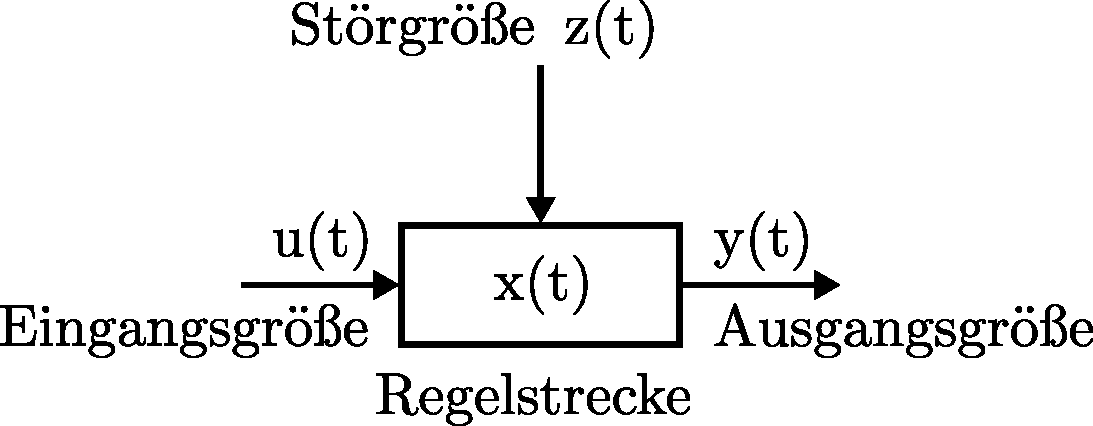
\includegraphics[width=0.5\linewidth]{Abbildungen/Grundbegriffe/PDF/DynamischesSystem.pdf}
	\caption{Dynamisches System als Beschreibung eines physikalischen Prozess}
	\label{fig:dynamischessystem}
\end{figure}
%
In Tabelle \ref{tab:beispieledynsystem} werden einige Beispiele gegeben, welche technische Systeme aus unserem Alltag mit den Kenngrößen aus Abbildung \ref{fig:dynamischessystem} verknüpfen.
%
\begin{table*}[h]\centering
	\ra{1.3}
	\caption{Beispiele für dynamisches Systeme und ihre zugehörigen Systemgrößen}
	\begin{tabular}{@{}llll@{}}\toprule
		Dynamisches System & $u(t)$ & $y(t)$ & $z(t)$ \\ \bottomrule\bottomrule
		Gleichstrommaschine & Ankerspannung & Drehzahl & Lastmoment \\
		Raumheizung & Thermostatstellung & Raumtemperatur & Außentemperatur \\
		Füllstandsregelung & Zugflussventilstellung & Füllhöhe & Abfluss \\
		Noise-Cancelling & Gegenmembran & Signal-Rauschverhältnis & Umgebungsgeräusche\\
		Pupille im Auge & Pupillenweite & Lichteinfall & Krankheiten, Alkohol\\
		Population & Raubtiere & Anzahl der Beutetiere & Jäger (Mensch)\\
		\bottomrule
	\end{tabular}
	\label{tab:beispieledynsystem}
\end{table*}\newpage
%
\textbf{Allgemein gilt:} Die Voraussetzung für den Einsatz einer Regelung ist ein bestenfalls mathematisch beschreibbarer Zusammenhang zwischen $u(t)$ und $y(t)$. Zudem sind weitere Informationen über die Wirkung und den Wert der jeweiligen Größen notwendig.\\\\
%
Schematischer Ablauf einer Regelung \cite{Lunze10}:
\begin{itemize}
	\item[1] Messen der Regelgröße $y(t)$: Dies erfolgt entweder direkt mit einem Sensor, oder wird aus messbaren Größen berechnet.
	\item[2] Vergleich zwischen Führungsgröße $w(t)$ und Regelgröße $y(t)$: Die Differenz dieser beiden Größen wird als Regeldifferenz $e(t)=w(t)-y(t)$ bezeichnet.  
	\item[3] Bestimmung der Stellgröße und Beeinflussung des Eingangs $u(t)$ der Regelstrecke: Dies erfolgt in der Regel unter Berücksichtigung der dynamischen Eigenschaften des Systems. 
\end{itemize}
%
An dieser Stelle sei darauf hingewiesen, dass die Rückführung das zentrale Element der Regelung darstellt \cite{Lunze10}.
%
%###############################################################################
\section{Historische Beispiele der Regelungstechnik}
%###############################################################################
%
\subsection{Antike Wasseruhr}
%
Die ersten praktischen Einsatzgebiete der Regelungstechnik waren mechanische oder fluidmechanische Konstruktionen. 
%
\begin{figure}[h]
	\centering
	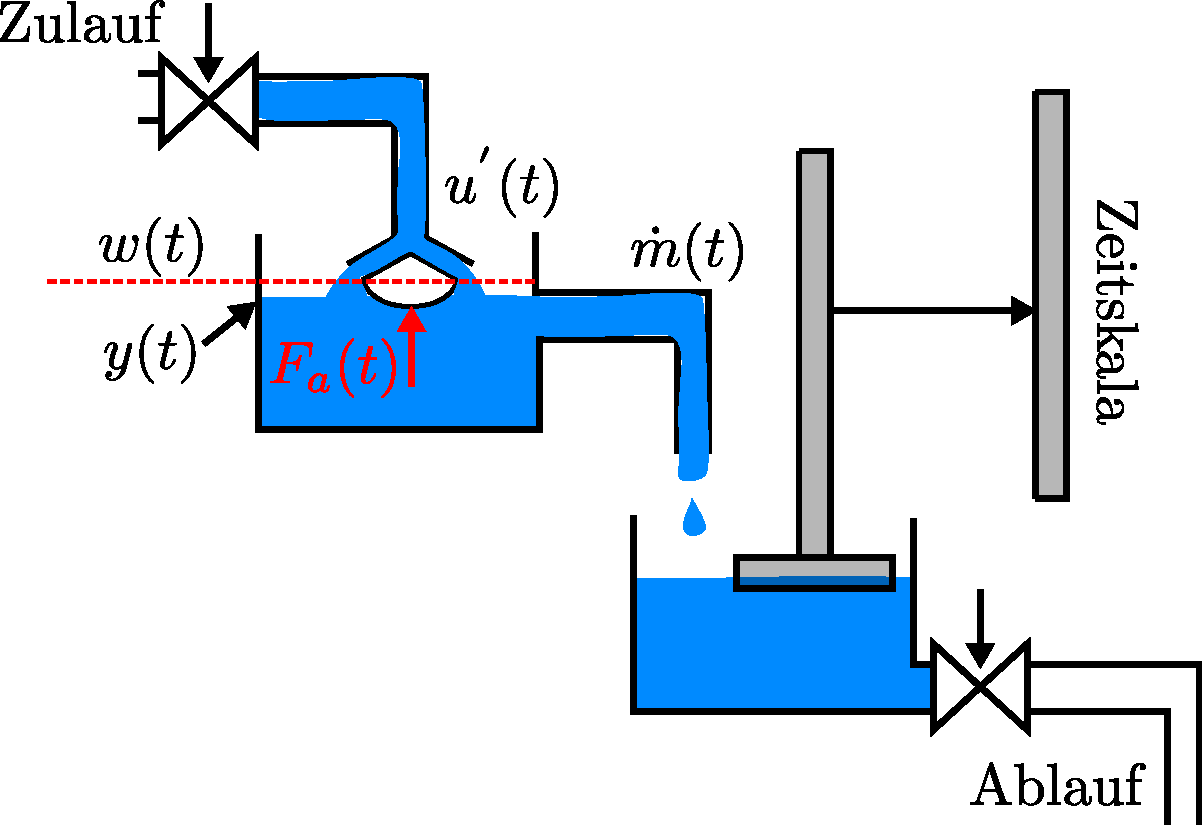
\includegraphics[width=0.6\linewidth]{Abbildungen/Grundbegriffe/PDF/HistorischeSystemeWasseruhr.pdf}
	\caption{Prinzipdarstellung einer antiken Wasseruhr, welche in dieser oder ähnlicher Form zwischen 1500-300 Jahre B.C. zum Einsatz kamen}
	\label{fig:wasseruhr}
\end{figure}
%
Zwar war die Regelungstechnik als solche noch nicht bekannt, ihre Grundprinzipien fanden jedoch schon sehr früh Anwendung, wie z.B. in Wasseruhren \cite{Lewis00,Landes00}. Der prinzipielle Aufbau solch einer Wasseruhr ist in Abbildung \ref{fig:wasseruhr} dargestellt. 
%
Das Regelungsziel war im Falle der Wasseruhr eine gleichmäßige Befüllung des unteren Behälters. Ein Schwimmer mit aufgesetztem Stab bewegt sich durch diese Füllstandsänderung an einer Zeitskala entlang. Je gleichmäßiger sich also der untere Behälter füllt, umso geringer sind die Unterschiede der gezählten Stunden über den Tag. Aus Regelungstechnischer Sicht ist das obere Becken die Regelstrecke:
%
\begin{itemize}
%
	\item Der Wasserzufluss $u^{'}(t)$ wird als konstant angenommen. Der Zufluss $u(t)$ in den oberen Behälter wird durch einen Schwimmer geregelt, welcher durch seine Auftriebskraft relativ zum Pegel als Ventil wirkt.
	%
	\item Somit ist der Sollwert $w(t)$ ein fester Pegel, welcher zu einem vordefiniertem Durchfluss an Wasser $\dot{m}(t)$ führt.
	%
	\item Die Regeldifferenz ergibt sich aus dem Sollwert und dem tatsächlichen Pegel $e(t)=w(t)-y(t)$
	%
	\item Als Eingang auf dass Stellglied (Schwimmer) wirkt die Auftriebskraft $F_{a}(t)$
\end{itemize}
%
\subsection{Fliehkraftregler von James Watt}
%
Ein mechanisches Beispiel wurde von James Watt um 1788 auf der Basis des Prinzips von rotierenden Körpern entwickelt \cite{Unbehauen08}. Der sogenannte Fliehkraftregler war in der Lage, die Drehzahl Watt's Dampfmaschinen zu regeln und so konstant zu halten. Der prinzipielle Aufbau der Regelung ist in Abbildung \ref{fig:fliehkraftregler} dargestellt.
%
\begin{figure}[h]
	\centering
	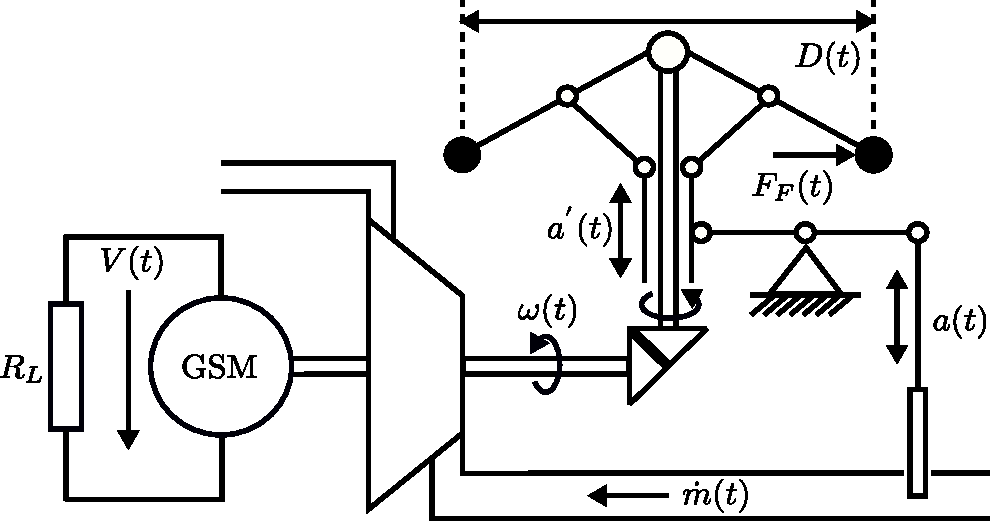
\includegraphics[width=0.83\linewidth]{Abbildungen/Grundbegriffe/PDF/HystorischeSystemeFliehkraft.pdf}
	\caption{Prinzipdarstellung einer Dampfmengenregelung durch einen Fliehkraftregler (Größen der einzelnen Komponenten, nicht maßstabsgetreu)}
	\label{fig:fliehkraftregler}
\end{figure}
%
Auf der linken Seite der Abbildung \ref{fig:fliehkraftregler} ist eine Gleichstrommaschine darstellt, welche im 18 Jahrhundert noch immer für die Generation von Elektrizität genutzt wurde, um Haushalte und die Industrie zu versorgen. Die Ausgangsspannung der Gleichstrommaschine musste für diesen Fall konstant geregelt werden, um eine gleichbleibende Versorgung der angeschlossenen Verbraucher sicherzustellen. Spannungsschwankungen machten sich sofort in der Helligkeit von Glühlampen oder der Drehzahl der angeschlossenen Maschinen in der Industrie bemerkbar. Da die Drehzahl der Gleichstrommaschine (bei Vernachlässigung der Verluste) der Gleichung \ref{eq:gleichstrommaschine}
%
\begin{align}
	V(t) = \phi\,\omega \label{eq:gleichstrommaschine}
\end{align}
%
folgt, kann dies über eine Regelung der Drehzahl erreicht werden. Im rechten Teil der Abbildung \ref{fig:fliehkraftregler} ist der angesprochenen Fliehkraftregler dargestellt. Die Funktion des Reglers kann wie folgt beschrieben werden:
%
\begin{itemize}
%
\item Eine Rotation der Gelenkstangen mit der Kreisfrequenz $\omega(t)$, welche über ein Kegelzahnrad von der Welle der Dampfmaschine angetrieben werden, führt durch die Fliehkraft $F_{F}(t)$ zu einem konstanten Kugelabstand $D(t)$.
%
\item Ändert sich die Kreisfrequenz $\omega(t)$, so ändert sich auch die Fliehkraft $F_{F}(t)$ und somit durch die Gelenkkonstruktion der Abstand $D(t)$ der beiden Gewichte des Reglers.
%
\item Das mechanische Umlenksystem übersetzt den Abstand $D(t)$ über  die Position $a^{'}(t)$ in die Dampfventilstellung $a(t)$.
%
\item Über die Dampfventilstellung $a(t)$ wird die Dampfmenge $\dot{m}(t)$ und somit das Drehmoment bzw. die Drehzahl der Dampfturbine geregelt.  
%
\end{itemize}
%
%
%##############################################################
\subsection{Regelungstechnik in der Neuzeit bis Heute}
%##############################################################
%
Seit den eher intuitiven Ansätzen regelungstechnischer Apparate sind viele mathematische und technische zusammenhänge erforscht worden, die heute einen wesentlich differenzierten und analytischen Blick auf die Regelungstechnik erlauben. Zunächst bedarf es somit einer Einordnung der Analysen und Grundlagenarbeiten, welche im weiteren zur modernen Regelungstechnik geführt haben \cite{Zom13}.
%
\begin{itemize}
	\item 1782 Jozef Maximili\'an Petzval, Pierre-Simon Laplace: \textit{Laplace-Transformation}
	\item 1868 James Clerk Maxwell: \textit{On Governors}, theoretische Betrachtung des Fliehkraftreglers
	\item 1877 Edward J. Routh: \textit{Treatise on the stability of a given state of motion}, Arbeit zum Stabilitätsbegriff linearer Systeme
	\item 1892 Aleksandr M. Lyapunov: \textit{The general problem of the stability of motion}, Verallgemeinerung der Stabilitätsbegriffes für beliebige dynamische Systeme
	\item 1895 Adolf Hurwitz: \textit{Über die Bedingungen unter welchen eine Gleichung nur Wurzeln mit negativen reellen Teilen besitzt.} (Routh-Hurwitz-Kriterium)
	\item 1932 Harry Nyquist: \textit{Regeneration theory}
	\item 1942 J. G. Ziegler, N. B. Nichols: \textit{Optimum settings for automatic controllers}, heuristische Einstellregeln für PID-Regler
	\item 1945 Hendrik W. Bode: \textit{Network analysis and feedback aplifier design}, 
	\item 1961 Rudolf E. K\'alm\'an, Richard S. Bucy: \textit{New results in linear filtering and prediction theory}, der K\'alm\'an Filter begründet den Zeitpunkt der modernen Regelungstechnik
\end{itemize}
%
Besonders durch die theoretischen Arbeiten von Petzval und Laplace in der Laplace-Transformation, aber auch die technischen Untersuchungen zum Fliehkraftregler von Maxwell konnten nun theoretische Konstrukte der Regelungstechnik entwickelt werden. Bis ins Jahr 1940 hatte sich die Regelungstechnik dann zur einer eigenständigen Wissenschaft etabliert. In dieser Vorlesung werden klassische Verfahren der Regelungstechnik eingeführt, welche sich bis 1960 entwickelt hatten.\\\\
%
In der heutigen Zeit ist die Regelungstechnik auch aus unserem Alltag nicht mehr weg zu denken. Unsere batteriebetriebenen Smart-Phones besitzen geregelte Spannungswandler, welche den unterschiedlichen Prozessoren und Komponenten bedarfsgerecht ihre Versorgung bereitstellen. Moderne Personen-Kraft-Wagen (PKW) besitzen Geschwindigkeitsregeleinrichtungen, um per Knopfdruck eine gewisse Fahrgeschwindigkeit einzustellen. 
%
%\footnote{Schottischer Mathematiker/Physiker. Hat die Theorie der Elektrodynamik entwickelt, und somit als erster Mensch den Zusammenhang %zwischen Elektriziät und Magnetismus mathematisch beschrieben. Die Hauptergebnisse seiner Arbeit sind als Maxwellsche Gleichungen bekannt %\cite{Maxwell54}.} 
%
\newpage
%
%##############################################################
\section{Struktur einer Regelung}
%##############################################################
%
%##############################################################
\subsection{Vollständiger Wirkungsplan einer Regelung}
%##############################################################
%
Grundsätzlich gibt es mehrere Möglichkeiten, um eine Regelung zu beschreiben. Zum einen kann sie durch das Aufstellen von mathematischen Gleichungssystemen erfolgen. Dies ist in den meisten Fällen zwar notwendig, jedoch für die strukturelle Aufbereitung zunächst nicht Zielführend. Deshalb wird an dieser Stelle der Wirkungsplan einer Regelung nach DIN IEC 60050-351 (ehemals DIN 19226-4) \cite{DKE14} eingeführt (vlg. Abbildung~\ref{fig:regelkreisdin}).
%
\begin{figure}[h]
	\centering
	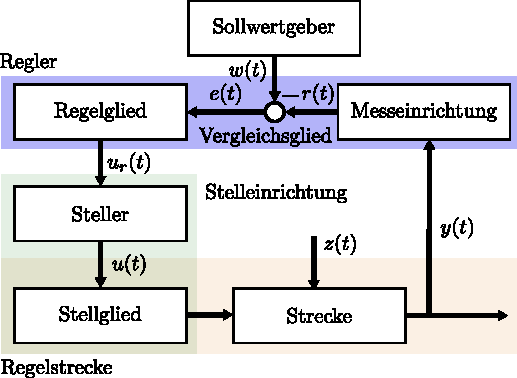
\includegraphics[width=0.70\linewidth]{Abbildungen/Grundbegriffe/PDF/VollstWirkungsplan.pdf}
	\caption{Wirkungsplandarstellung einer Regelung nach DIN}
	\label{fig:regelkreisdin}
\end{figure}\\
%
Folgende Begrifflichkeiten sollen hier näher erläutert werden (siehe auch\cite{Foellinger94}\cite{MSF05}):
\begin{itemize}
\item Systemblock Regeleinrichtung
\begin{description}
\item \underline{Messeinrichtung:} Hat die Aufgabe, die allgemeine Messgröße (Weg, Strom, Drehzahl, Druck) in eine für das Regelungssystem verarbeitbare Form umzuwandeln. Hierbei muss beachtet werden, dass Messglieder auch ein Übertragungsverhalten besitzen.
%
\item \underline{Sollwertgeber:} Erzeugt die Führungsgröße des Regelkreises und gibt sie an die Vergleichsstelle zwischen Messeinrichtung und Regelglied weiter
\item \underline{Vergleichsglied:} Bildet die Regeldifferenz $e(t)$ aus Ausgangsgröße $y(t)$ und Sollwert $w(t)$.
\item \underline{Regelglied:} Dieser Teil der Regeleinrichtung berechnet aus der Regeldifferenz $e(t)$ eine Referenzgröße für den Steller. Dieser Berechnung liegt das Regelgesetz zugrunde.
\end{description}
%
\item Systemblock Stelleinrichtung
\begin{description}
	\item \underline{Steller:} Ist die ausführende Funktionseinheit und wandelt das Ausgangssignal des Regelglieds in ein für das Stellglied verständliches Signal um.
	%
	\item \underline{Stellglied:} Ist meist Teil der Regelstrecke und setzt das Stellsignal um, indem es in die zu regelnden Größen $\boldsymbol{x}(t)$ eingreift. 
\end{description}
%
\item Systemblock Regelstrecke
\begin{description}
	\item \underline{Strecke:} Ist der Teil des Regelkreises, in welchem sowohl die Regelgrößen beeinflusst, als auch die Messgrößen abgegriffen werden. Oft wird die Regelstrecke auch als der zu regelnde Prozess bezeichnet.
\end{description}
\end{itemize}
%
%##############################################################
\subsection{Vereinfachter Wirkungsplan einer Regelung}
%##############################################################
%
Wird die Messeinrichtung und das Stellglied als Teil der Regelstrecke angesehen und der Steller in die Regeleinrichtung integriert, ergibt sich das folgende vereinfachte Blockschaltbild (vgl. Abbildung~\ref{fig:regelkreiseinfach}), welches den Wirkungsplan auf seine wesentlichen Komponenten vereinfacht \cite{MSF05}. 
%
\begin{figure}[h]
	\centering
	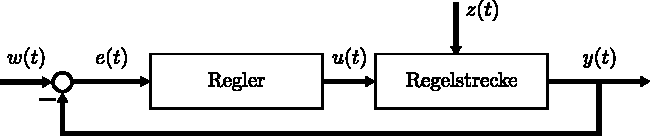
\includegraphics[width=0.9\linewidth]{Abbildungen/Grundbegriffe/PDF/VereinfWirkungsplan.pdf}
	\caption{Vereinfachte Wirkungsplandarstellung}
	\label{fig:regelkreiseinfach}
\end{figure}\\ 
%
Das Regelglied wird nun vereinfacht als 'Regler' bezeichnet und die Regelstrecke enthält nun die Messeinrichtung so wie das Stellglied.
%
%##############################################################
\subsection{Wirkungsplan am Beispiel einer Fahrstuhlregelung}
%##############################################################
%
Die Vorgehensweise zur Aufstellung des vollständigen und vereinfachten Wirkschaltplanes, soll nun Anhand einer Drehzahlregelung einer Gleichstrommaschine dargestellt werden (aus \cite{MSF05}, Beispiel 1.9). In Abbidung~\ref{fig:aufzug} ist zunächst der technische Prozess mit den jeweiligen Komponenten dargestellt.
%
\begin{figure}[ht!]
	\centering
	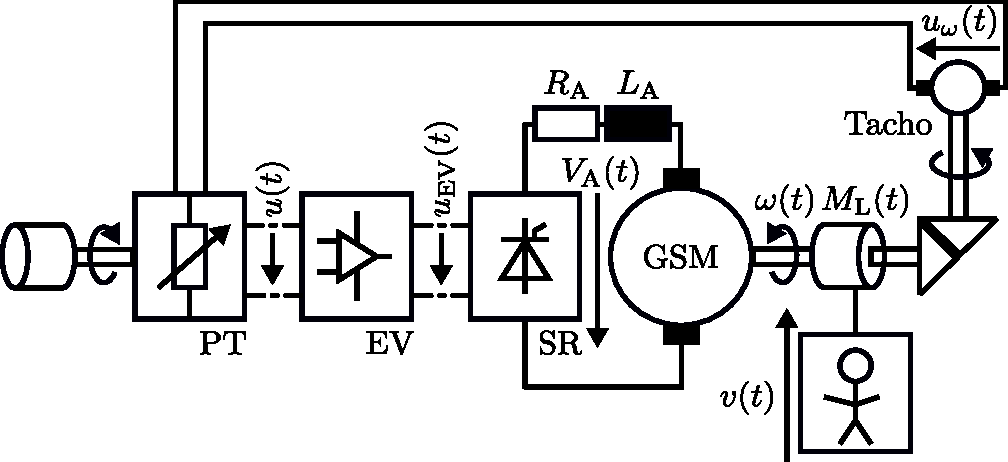
\includegraphics[width=0.83\linewidth]{Abbildungen/Grundbegriffe/PDF/Fahrstuhlregelung.pdf}
	\caption{Regelung der Fahrgeschwindigkeit eines Aufzuges (nach \cite{MSF05} Bild 1.14 a) )}
	\label{fig:aufzug}
\end{figure}
%
\begin{Aufgaben}{}{}
	\begin{itemize}
		\item \textit{Blockschaltbild der Fahrstuhlregelung}
	\end{itemize}
\end{Aufgaben}
%
Wird nun der technische Prozess durch seine Wirkungsblöcke dargestellt, ergibt sich folgender vollständiger Wirkungsplan (Abbildung~\ref{fig:aufzugwirkvoll}).  
%
\begin{figure}[ht!]
	\centering
	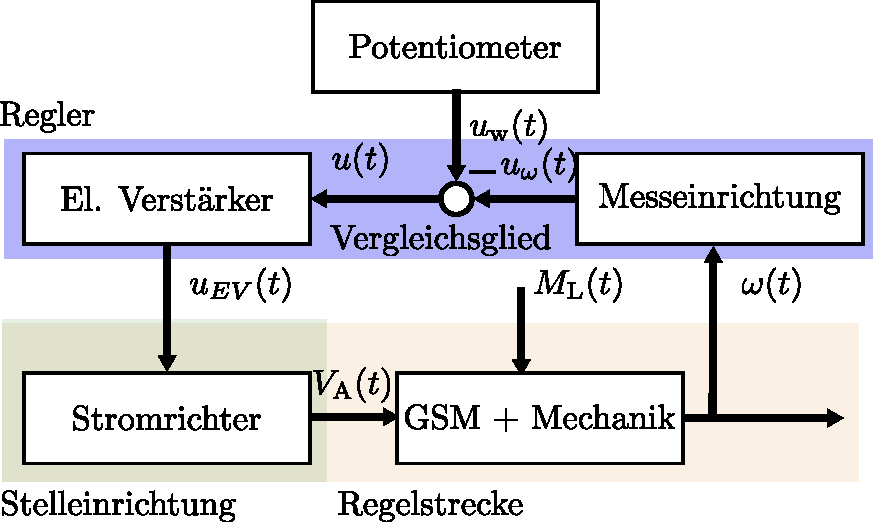
\includegraphics[width=0.7\linewidth]{Abbildungen/Grundbegriffe/PDF/FahrstuhlregelungWirkungsplan.pdf}
	\caption{Vollständige Wirkungsplandarstellung der Fahrstuhlregelung (nach \cite{MSF05} Bild 1.14 b)}
	\label{fig:aufzugwirkvoll}
\end{figure}
%
Durch die Kombination von Stromrichter, Gleichstrommotor, Aufzug und Tachogenerator ergibt sich der vereinfachte Wirkungsplan der Fahrstuhlregelung. Der Vorgang wird an dieser Stelle nicht weiter ausgeführt, da er dem allgemeinen Prinzip folgt.
%
%#########################################################################################################
\section{Prinzip der Steuerung in der offenen Wirkungskette}
%#########################################################################################################
%
Eine Steuerung wird meist als offene Wirkungskette bezeichnet und besitzt keine Rückführung der Regelgröße, wie in Abbildung~\ref{fig:steuerung} dargestellt.
%
\begin{figure}[h]
	\centering
	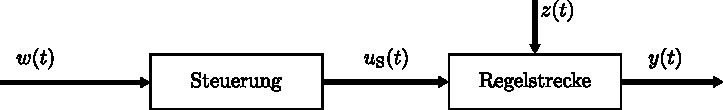
\includegraphics[width=0.95\linewidth]{Abbildungen/Grundbegriffe/PDF/Steuerung.pdf}
	\caption{Prinzip der Steuerung in der offenen Wirkungskette ohne Rückführung}
	\label{fig:steuerung}
\end{figure}
%
Grundsätzlich kann die Zielvorgabe, nämlich eine Regelgröße auf einen bestimmten Wert einzustellen, auch ohne Rückführung erreicht werden. Sind sämtliche Störungen abgeklungen oder vernachlässigbar $z(t)=0,\forall t \in\{0+,\cdots,\infty\}$, so kann über die Beziehung \eqref{eq:steuerung}
%
\begin{align}
y(t) = f(u(t))\label{eq:steuerung}
\end{align}
%
Berechnet werden, welche Führungsgröße $w(t)$ die Stellgröße $u(t)$ so beeinflusst, dass \eqref{eq:führung} gilt
%
\begin{align}
w(t) = y(t)\label{eq:führung}
\end{align}
%
Dies ist in vielen Fällen nur schwer möglich, da $f(\cdot)$ meist durch eine Differentialgleichung beschrieben werden muss. Das inverse Modell kann nur erstellt werden, wenn die dynamischen Eigenschaften der Regelstrecke ausreichend bekannt sind. Eine Steuerung kann in diesem Fall erstellt werden durch die Vorschrift \eqref{eq:inversion}. 
%
\begin{equation}
\begin{aligned}
u(t) &= f^{-1}(w(t))\\
y(t) &= f(u(t))=f\left(f^{-1}(w(t))\right)=w(t)\label{eq:inversion}
\end{aligned}
\end{equation}
%
Jedoch ist es möglich, dass die Funktion $f^{-1}(\cdot)$ nicht existiert, da $f(\cdot)$ nicht invertierbar ist. Ist dies der Fall, kann nur eine Annäherung $\tilde{f}^{-1}(\cdot)$ berechnet werden. Diese Näherung bewirkt, dass nur die Forderung $y(t)\approx w(t)$ erreicht werden kann.\\
%
Es wir somit recht schnell klar, dass die Regelung wesentliche Vorteile gegenüber einer Steuerung in der offenen Wirkungskette besitzt. Vor allem ist hier jedoch die Sollwertfolge zu nennen, deren Funktion in der geschlossen Wirkungskette trotz unterschiedlicher Eigenschaften der Regelstrecke erhalten bleibt \cite{Lunze10}. Eine Regelung hat grundsätzlich Vorteile:
%
\begin{itemize}
	\item im Falle einer instabilen Regelstrecke.
	\item bei nicht messbaren Störungen. 
	\item falls die statischen und dynamischen Parameter der Strecke nicht genau bekannt sind.
	\item falls diese Parameter sich zeitlich ändern.
\end{itemize} 
%
%#########################################################
\subsection{Anwendung im Regelkreis als Vorsteuerung}
%#########################################################
%
Nichts desto trotz findet das Prinzip der Steuerung in der offenen Wirkungskette in moderne Regelkreise Einzug. Ein Beispiel hierfür ist die Vorsteuerung, welche als weiterer Freiheitsgrad der Regelung genutzt werden kann, um Sollwerte schneller zu erreichen \cite{Lunze10}. Sowohl der Regler als auch die Vorsteuerung erhalten den gleichen Sollwert $w(t)$ und schalten diesen unterschiedlich auf die Strecke auf, wie in Abbildung~\ref{fig:vorsteuerung} dargestellt.
%
\begin{figure}[h]
	\centering
	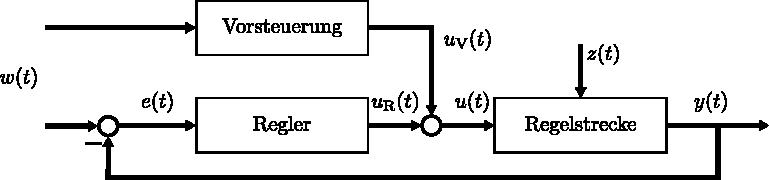
\includegraphics[width=0.95\linewidth]{Abbildungen/Grundbegriffe/PDF/Vorsteuerung.pdf}
	\caption{Nutzung einer Steuerung, um die Sollwertfolge im geschlossenen Regelkreis zu verbessern}
	\label{fig:vorsteuerung}
\end{figure}
%
Die Eingangsgröße $u(t)$ auf die Regelstrecke teilt sich nun in einen Anteil des Reglers $u_{\text{R}}(t)$ und in einen Anteil der Vorsteuerung $u_{\text{V}}(t)$ auf.
%
Beide Kreise können separat entworfen werden, wobei beim Regelkreis nun das Augenmerk auf die Stabilisierung und Störkompensation und bei der Vorsteuerung auf eine möglichst gute Sollwertfolge gelegt wird.\\

\textbf{Eigenschaften:}
\begin{itemize}
	\item Verbessert die Umschaltung zwischen zwei Arbeitspunkten.
	\item Erhöht die Freiheitsgrade in der Regelung.
	\item Sollwert kann meist schneller erreicht werden, als im Falle der 'einfachen' Regelung. 
\end{itemize}
%
%#########################################################
\subsection{Anwendung im Regelkreis als Störgrößenaufschaltung} 
%#########################################################
%
Ein weiteres Anwendungsfeld einer Steuerung ist die Störgrößenaufschaltung oder auch Störgrößenkompensation genannt \cite{Foellinger94,Lunze10}. Zu beachten ist, dass diese nur entworfen werden kann, wenn die zu kompensierenden Störungen $\tilde{z}(t)$ messbar sind \underline{bevor} sie auf die Regelstrecke wirken. Die Störgrößenkompensation im Regelkreis ist in Abbildung~\ref{fig:stoergroesse} dargestellt.
%
\begin{figure}[h]
	\centering
	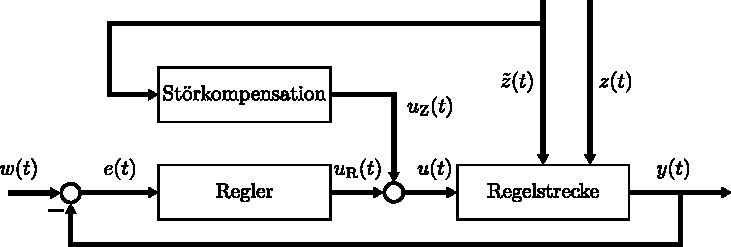
\includegraphics[width=0.95\linewidth]{Abbildungen/Grundbegriffe/PDF/StoerGroessen.pdf}
	\caption{Nutzung einer Störgrößenaufschaltung, um messbare Störung zu kompensieren.}
	\label{fig:stoergroesse}
\end{figure}
%
Ziel der Kompensation ist eine möglichst gute Unterdrückung der Störungswirkung $\tilde{z}(t)$ ohne das Führungsverhalten des Regelkreises wesentlich zu beeinflussen. Grundsätzlich kann jeder Regler auf Führungs- und Störverhalten optimiert werden, aber die Störunterdrückung ist in vielen Fällen effektiver.\\

\textbf{Eigenschaften:}
\begin{itemize}
	\item Realisierbar für Störungen die sich einfach messen lassen.
	\item Wirkung der Störung auf den Regelkreis kann unterdrückt werden.
	\item Eine 100\% Unterdrückung ist praktisch nicht möglich, da dynamische Systeme nicht invertierbar sind.
\end{itemize}
%
\begin{simulation}{}{}
	\begin{itemize}
		\item \textit{Kurze Einführung in Octave}
	\end{itemize}
\end{simulation}
%
%#########################################################
\section{Klassifikation von Regelungsaufgaben}
%#########################################################
%
%#########################################################
\subsection{Festwert- oder Störgrößenregelung}
%#########################################################
\label{sec:Klassifikation}
%
Eine Regelung kann zunächst durch ihre vorrangige Aufgabe klassifiziert werden. Diese Aufgabe kann z.B. die Störgrößenregelung bzw. Festwertregelung sein \cite{MSF05,Zacher17}. Dies bedeutet, dass der Sollwert der zu regelnden Strecke sich nicht wesentlich ändert. Jedoch sind immer wieder Störungen $z(t)$, welche auf die Strecke wirken, zu erwarten. Der Regelkreis sollte in diesem Fall ein gutes Störverhalten aufweisen. Die Systemantwort $h_{\text{z}}(t)$ auf eine Störgröße ist in Abbildung~\ref{fig:festwert} dargestellt.
%
\begin{figure}[h]
	\centering
	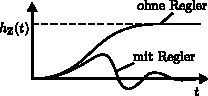
\includegraphics[width=0.4\linewidth]{Abbildungen/Grundbegriffe/PDF/FestwertRegelung.pdf}
	\caption{Typisches zeitliches Verhalten der Störsprungantwort $h_{\text{z}}(t)$, für den Fall ohne und mit Regelung}
	\label{fig:festwert}
\end{figure}
%
Es ist deutlich zu erkennen, dass ohne Regler eine bleibende Abweichung entstehen würde. Diese Abweichung ist im Regelkreis nicht erwünscht und sollte durch die geeignete Wahl des Reglers unterdrückt werden.
%
%#########################################################
\subsection{Folgereglung}
%#########################################################
%
Ändert der Sollwert sich zeitlich, so kann der Regelkreis als Folgeregelung entworfen werden. Die Regelungsaufgabe ist nun, die Regelgröße $y(t)$ dem Sollwert $w(t)$ nachzuführen. Die qualitative Beurteilung der Funktion erfolgt anhand des Führungsverhaltens des Regelkreises \cite{Lunze10}. 
%
\subsubsection{Führungssprungantworten und unterschiedliche Führungsgrößen}
%
Eine klassische Führungsgrößenänderungen ist die Sprungfunktion. Eine CNC-Fräse soll eine neue Position anfahren. Hierfür müssen die Servomotoren ohne Überschwingen und ohne bleibende Regelabweichung auf die neue Zielposition verfahren werden. Andernfalls würde zu viel oder zu wenig Material aus dem Werkstück gefräst werden. In Abbildung~\ref{fig:sprungantwort} ist dieser Sachverhalt exemplarisch dargestellt.
%
\begin{figure}[h]
	\centering
	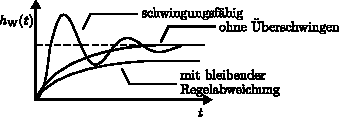
\includegraphics[width=0.65\linewidth]{Abbildungen/Grundbegriffe/PDF/Fuehrungssprung.pdf}
	\caption{Typisches zeitliches Verhalten der Führungssprungantwort $h_{\text{w}}(t)$, für unterschiedliche Reglerparameter}
	\label{fig:sprungantwort}
\end{figure}\\
%
Jedoch ist es gerade bei Servomotoren üblich, die Position mittels einer festgelegten Bahn zu erreichen. In diesem Fall kann eine lineare Änderung der Führungsgröße erfolgen, um den neuen Arbeitspunkt anzufahren. Das Verhalten des Regelkreises mit und ohne bleibende Regelabweichung ist in Abbildung~\ref{fig:anstiegsfunktion} dargestellt.
%
\begin{figure}[h]
	\centering
	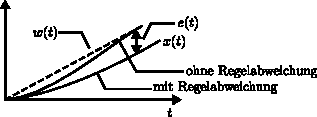
\includegraphics[width=0.65\linewidth]{Abbildungen/Grundbegriffe/PDF/Anstiegsfunktion.pdf}
	\caption{Lineare Führungsgrößenänderung $w(t)$}
	\label{fig:anstiegsfunktion}
\end{figure}
%
Eine weitere in der Praxis genutzte Führungsgröße ist die Parabelform. Diese Parabelform ist beispielsweise bei Industrierobotern zu finden \cite{Lunze10}. Die Position wird dort in Form eines Polynoms vorgegeben und muss durch den Regler eingehalten werden. In vielen Fällen wird diese Aufgabe durch die Kombination mit einer Vorsteuerung gelöst. Das prinzipielle Verhalten ist in Abbildung~\ref{fig:parabelfunktion} dargestellt.
%
\begin{figure}[h]
	\centering
	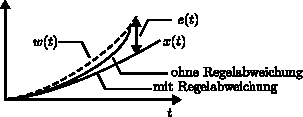
\includegraphics[width=0.65\linewidth]{Abbildungen/Grundbegriffe/PDF/Parabelfunktion.pdf}
	\caption{Parabelförmige Führungsgrößenänderung $w(t)$}
	\label{fig:parabelfunktion}
\end{figure}
%
\underline{Anmerkung:} Es gibt Anwendungen, bei denen trotz der Nutzung einer linearen oder polynomförmigen Führungsgröße keine bleibende Regelabweichung zulässig ist.  
\begin{itemize}
	\item Fliegende Schere: Durchschneiden einer sich bewegenden Papierbahn.
	\item Wiederholgenauigkeit von Trajektorien bei Industrierobotern in der Automobilfertigung.
\end{itemize}
%
\begin{Summary}{}{}
	\begin{itemize}
	\item \textit{Welche Komponenten sind im Regelkreis nach DIN enthalten?}
	\begin{itemize}
		\item \textit{Zeichnen und benennen Sie sämtliche Komponenten}
		\item \textit{Kreisen Sie die jeweiligen Gruppen ein}
	\end{itemize}
	\item \textit{Was ist der Unterschied zwischen offener Wirkungskette und geschlossenem Regelkreis?}
	\item \textit{Für welche Anwendungszwecke kann eine Steuerung eingesetzt werden?}
	\begin{itemize}
		\item \textit{Suchen sie zwei technische Beispiele für Vorsteuerungen aus gängiger Literatur}
	\end{itemize}
	\item \textit{Wie können Regelungsaufgaben grundsätzlich klassifiziert werden?}
	\item \textit{Welche Auswirkungen haben bleibende Regelabweichungen?}
	\end{itemize}
\end{Summary}
%
%%#######################################################################
%\section{Qualitative and Quantitative Anforderungen and den Regelkreis}
%%#######################################################################
%%
%Bisher wurden die notwendigen Begriffe und die Wirkungsweise der Regelung eingeführt. Nun stellt sich die Frage wie eine Regelung zu entwerfen ist. Hierfür müssen zunächst die Anforderungen definiert und spezifiziert werden.
%%
%\subsection{Der Regelkreis als Entwurfsaufgabe}
%%
%Grundsätzlich können die Anforderungen an einen Regelkreis in vier Hauptgruppen unterteilt werden \cite{Lunze10}
%%
%\begin{itemize}
%	\item Stabilität
%	\item Störkompensation und Sollwertfolge
%	\item Dynamisches Verhalten
%	\item Robustheit 
%\end{itemize}
%##############################################################################
\chapter{Modellbildung}
\label{chap:Modellbildung}
%##############################################################################
%
Die Modellbildung befasst sich mit der mathematischen Beschreibung technischer Systeme. Das hieraus resultierende mathematische Modell soll das Verhalten zwischen Eingangsgröße $u(t)$ und Ausgangsgröße $y(t)$ mit gewünschter Genauigkeit beschreiben. Die meisten technischen Systeme lassen sich durch partielle oder gewöhnliche Differenzialgleichungen darstellen. Im folgenden soll anhand eines einfachen Beispiel die grundsätzliche Vorgehensweise veranschaulicht werden. 
%
%##############################################################################
\section{Einführendes Beispiel}
%##############################################################################
%
Dies soll zunächst anhand eines Beispiels demonstriert werden (basierend auf \cite{Foellinger94}). In Abbildung~\ref{fig:rlglied} auf der linken Seite ist ein $RL$-Glied, bestehend aus Induktivität $L$ und ohmschen Widerstand $R$ dargestellt.
%
\begin{figure}[h]
	\centering
	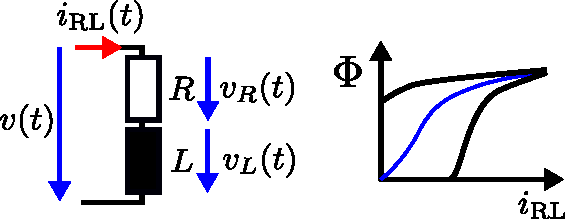
\includegraphics[width=0.5\linewidth]{Abbildungen/Modellbildung/PDF/RLglied.pdf}
	\caption{Reihenschaltung aus Induktivität und Widerstand}
	\label{fig:rlglied}
\end{figure}
%  
Unter Berücksichtigung der Eisensättigung der realen Induktivität würde sich für den magnetischen Fluss eine exemplarische nichtlineare Kurve, wie in Abbildung~\ref{fig:rlglied} ergeben.
Im ersten Schritt werden nun die mathematischen Gleichungen des Systems beginnend mit dem Maschensatz aufgestellt \eqref{eq:diffglrl}.
%
\begin{equation}
\begin{aligned}
	&v(t)=v_{\text{R}}(t)+v_{\text{L}}(t).\\
\end{aligned}
\end{equation}
%
Danach können die Gleichungen für die einzelnen Elemente aufgestellt werden
%
\begin{equation}
\begin{aligned}	
	&v_{\text{R}}(t) = R\cdot i_{\text{RL}}(t)\\
	&v_{\text{L}}(t) = \frac{\text{d}\Phi(t)}{\text{d}t}\\
	&i_{\text{RL}}(t) = f\left(\Phi(t)\right) &&\text{Nichtlinear Zusammenhang}\label{eq:diffglrl}
\end{aligned}
\end{equation}
%
Im zweiten Schritt können die aufgestellten Systemgleichungen in einzelnen Blöcken grafisch dargestellt und zusammengeführt werden. Dies erleichtert die spätere Darstellung im sogenannten Blockschaltbild. Zunächst muss jedoch noch definiert werden welche Größe den Eingang und welche den Ausgang des Systems beschreiben soll. In diesem Beispiel nutzen wir $v(t)$ als Eingang, das dieser direkt im System beeinflussbar ist und $i_{\text{RL}}(t)$ als Ausgang. Alle Gleichungen aus \eqref{eq:diffglrl} werden einem Block zugeordnet und ergeben folgende Schaltbilder:
%
%\begin{figure}[h]
%	\begin{minipage}{0.5\textwidth}
%	\begin{itemize}
%		\item Kennlinienglied $i_{\text{RL}}=f(\Phi(t))$
%	\end{itemize}
%	Kennlinienglieder beschreiben einen statischen funktionalen Zusammenhang zwischen Eingang und Ausgang (in der Regel nichtlinear).
%	\end{minipage}\hfill
%	\begin{minipage}{0.5\textwidth}
%		\centering
%		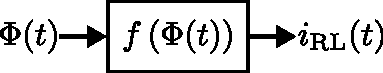
\includegraphics[width=0.7\textwidth]{Abbildungen/Modellbildung/PDF/Kennlinienglied.pdf}
%	\end{minipage}
%\end{figure}
%%
%  \begin{figure}[h]
%	\begin{minipage}{0.5\textwidth}
%		\begin{itemize}
%			\item Proportionalglied $v_{\text{R}}=R\cdot i_{\text{RL}}$
%		\end{itemize}
%		Proportionalglieder beschreiben einen statischen funktionalen Zusammenhang zwischen Eingang und Ausgang (linearer Fall).
%	\end{minipage}
%	\begin{minipage}{0.5\textwidth}
%		\centering
%		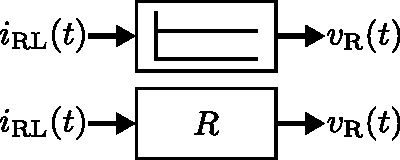
\includegraphics[width=0.7\textwidth]{Abbildungen/Modellbildung/PDF/Proportionalglied.pdf}
%	\end{minipage}
%\end{figure} 
%%
%  \begin{figure}[h]
%	\begin{minipage}{0.5\textwidth}
%		\begin{itemize}
%			\item Differentationsglied $v_{\text{L}}=\frac{\text{d}\Phi(t)}{\text{d}t}$
%		\end{itemize}
%		Berechnet die Ableitung des Eingangsignals und stellt es am Ausgang bereit.
%	\end{minipage}\hfill
%	\begin{minipage}{0.5\textwidth}
%		\centering
%		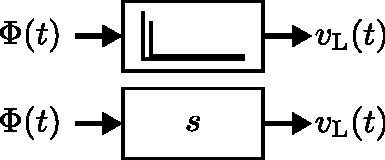
\includegraphics[width=0.7\textwidth]{Abbildungen/Modellbildung/PDF/Differnzierglied.pdf}
%	\end{minipage}
%\end{figure} 
%%
%  \begin{figure}[h]
%	\begin{minipage}{0.5\textwidth}
%		\begin{itemize}
%			\item Integrationsglied $\Phi =\frac{1}{T}\int v_{\text{L}}(t)\text{d}t$
%		\end{itemize}
%	Integrationsglieder integrieren den Systemeingang auf und bilden daraus den Systemausgang. Die Variable $T$ gibt die Integrationszeitkonstante an.
%	\end{minipage}\hfill
%	\begin{minipage}{0.5\textwidth}
%		\centering
%		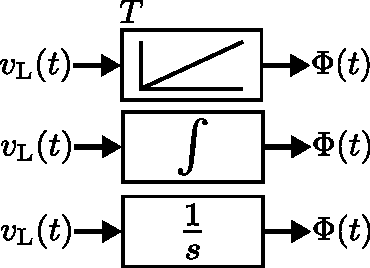
\includegraphics[width=0.7\textwidth]{Abbildungen/Modellbildung/PDF/Integratorglied.pdf}
%	\end{minipage}
%\end{figure} 
%%
%  \begin{figure}[h]
%	\begin{minipage}{0.5\textwidth}
%		\begin{itemize}
%			\item Summationsglied $v_{\text{L}}=v-v_{\text{R}}$
%		\end{itemize}
%		Durch ein Summationsglied kann die Addition oder Subtraktion zweier Größen dargestellt werden.
%	\end{minipage}\hfill
%	\begin{minipage}{0.5\textwidth}
%		\centering
%		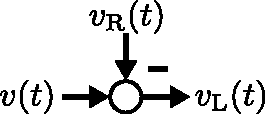
\includegraphics[width=0.5\textwidth]{Abbildungen/Modellbildung/PDF/Summationsglied.pdf}
%	\end{minipage}
%\end{figure}
%

\begin{figure}[h]
  \begin{subfigure}[c]{\textwidth}
	\begin{minipage}{0.5\textwidth}
	\begin{itemize}
		\item Kennlinienglied $i_{\text{RL}}=f(\Phi(t))$
	\end{itemize}
	Kennlinienglieder beschreiben einen statischen funktionalen Zusammenhang zwischen Eingang und Ausgang (in der Regel nichtlinear).
	\end{minipage}\hfill
	\begin{minipage}{0.5\textwidth}
		\centering
		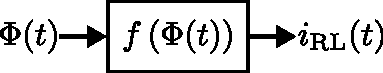
\includegraphics[width=0.7\textwidth]{Abbildungen/Modellbildung/PDF/Kennlinienglied.pdf}
	\end{minipage}
\end{subfigure}
%
%\vspace{1cm}
%
  \begin{subfigure}[c]{\textwidth}
	\begin{minipage}{0.5\textwidth}
		\begin{itemize}
			\item Proportionalglied $v_{\text{R}}=R\cdot i_{\text{RL}}$
		\end{itemize}
		Proportionalglieder beschreiben einen statischen funktionalen Zusammenhang zwischen Eingang und Ausgang (linearer Fall).
	\end{minipage}
	\begin{minipage}{0.5\textwidth}
		\centering
		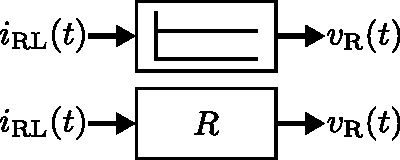
\includegraphics[width=0.7\textwidth]{Abbildungen/Modellbildung/PDF/Proportionalglied.pdf}
	\end{minipage}
\end{subfigure} 
%
%\vspace{0.5cm}
%
  \begin{subfigure}[c]{\textwidth}
	\begin{minipage}{0.5\textwidth}
		\begin{itemize}
			\item Differentationsglied $v_{\text{L}}=\frac{\text{d}\Phi(t)}{\text{d}t}$
		\end{itemize}
		Berechnet die Ableitung des Eingangsignals und stellt es am Ausgang bereit.
	\end{minipage}\hfill
	\begin{minipage}{0.5\textwidth}
		\centering
		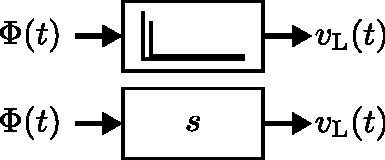
\includegraphics[width=0.7\textwidth]{Abbildungen/Modellbildung/PDF/Differnzierglied.pdf}
	\end{minipage}
\end{subfigure} 
%
%\vspace{1cm}
%
  \begin{subfigure}[c]{\textwidth}
	\begin{minipage}{0.5\textwidth}
		\begin{itemize}
			\item Integrationsglied $\Phi =\frac{1}{T}\int v_{\text{L}}(t)\text{d}t$
		\end{itemize}
	Integrationsglieder integrieren den Systemeingang auf und bilden daraus den Systemausgang. Die Variable $T$ gibt die Integrationszeitkonstante an.
	\end{minipage}\hfill
	\begin{minipage}{0.5\textwidth}
		\centering
		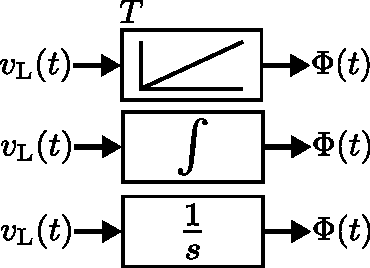
\includegraphics[width=0.7\textwidth]{Abbildungen/Modellbildung/PDF/Integratorglied.pdf}
	\end{minipage}
\end{subfigure} 
%
%\vspace{1cm}
%
  \begin{subfigure}[c]{\textwidth}
	\begin{minipage}{0.5\textwidth}
		\begin{itemize}
			\item Summationsglied $v_{\text{L}}=v-v_{\text{R}}$
		\end{itemize}
		Durch ein Summationsglied kann die Addition oder Subtraktion zweier Größen dargestellt werden.
	\end{minipage}\hfill
	\begin{minipage}{0.5\textwidth}
		\centering
		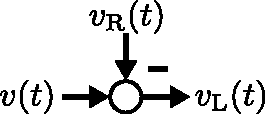
\includegraphics[width=0.5\textwidth]{Abbildungen/Modellbildung/PDF/Summationsglied.pdf}
	\end{minipage}
\end{subfigure}
\end{figure}
%
%\newpage
%
Durch Kombination der einzelnen Blöcke können nun die Gleichungen aus \eqref{eq:diffglrl} als Blockschaltbild dargestellt werden (Abbildung~\ref{fig:blockschaltbild}).
%
\begin{figure}[h]
	\centering
	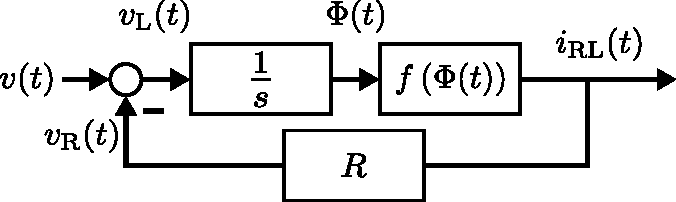
\includegraphics[width=0.65\linewidth]{Abbildungen/Modellbildung/PDF/Wirkschaltplan.pdf}
	\caption{Wirkschaltplan des dynamischen Verhaltens des RL-Glieds (vgl. \cite{Foellinger94})}
	\label{fig:blockschaltbild}
\end{figure}
%
Dieses erste anschauliche Beispiel hat nun vier Übertragungsglieder eingeführt, welche in der Darstellung von technischen Systemen genutzt werden können. Die Kennlinien in den Blöcken stellen die Antwort des Block Ausgangs auf einen Sprung am Eingang dar. Es stellt sich jedoch die Frage, wie Übertragungsglieder etwas allgemeiner klassifiziert werden können. Hierzu sollen die wichtigsten Merkmale im nächsten Kapitel dargestellt werden.
%
%##############################################################################
\section{Klassifikation von Übertragungsgliedern}
%##############################################################################
%
Ein Übertragungsglied beschreibt eine mathematische Abbildung zwischen Eingangsgröße $u(t)$ und Ausgangsgröße $y(t)$. Die Abbildung kann eine allgemeine Funktion sein z.B. $y(t)=u^{3}(t)$ aber eben auch eine Differentialgleichung. Letzteres bezieht sich auf den Fall, dass ein dynamisches System durch ein Übertragungsglied dargestellt werden soll. Übertragungsglieder können durch eindeutige Eigenschaften klassifiziert werden \cite{Foellinger94, Unbehauen08, Lunze10, Zacher17}, welche im Folgenden näher erläutert werden.
%
%##############################################################################
\subsection{Dynamik}
%##############################################################################
%
Wie schon im einführenden Beispiel (Abbildung~\ref{fig:rlglied}) dargestellt gibt es dynamische und statische Anteile in einem technischen System. Statische Anteile sind z.B.
%
\begin{itemize}
	\item Kennlinien für Magnetisierung, Materialfestigkeit, Federsteifigkeit, Reibkonstante (Reifen Bodenkontakt) etc.
	\item Falls die Dynamik eines Teilsystems wesentlich kleinere Zeitkonstanten aufweist, wie die anderen betrachteten Elemente und deren Einfluss auf das Gesamtverhalten vernachlässigbar ist. In diesem Fall wird meist nur die statische Verstärkung ($h(t)$ für $t\rightarrow \infty$) des vormals dynamischen Teilsystems betrachtet.
\end{itemize}
%
Im Falle eines statischen Anteils ist die Abbildung zwischen Ein- und Ausgang konstant und nicht von weiteren Einflussgrößen Abhängig. Dies ist beispielsweise ein Ansatz, wenn Dynamiken des betrachteten technischen Systems so schnell ablaufen, dass sie für deren Modellierung keine Rolle spielen. Bei einem dynamischen Übertragungsglied kann sich die Übertragungseigenschaft zwischen Ein- und Ausgang ändern. Grund für eine Systemdynamik sind die Energiespeicher in einem technischen System. Energiespeicher bewirken das einzelne Systemgrößen wie Spannung $v(t)$ oder Strom $i(t)$ sich nicht schlagartig ändern können. So ist beispielsweise in einer realen Induktivität Energie im magnetischen Feld gespeichert. Bei einer konstanten Eingangspannung würde nach \eqref{eq:diffglrl} der magnetische Fluß $\Phi$ linear, jedoch niemals sprungförmig ansteigen.
%
%############################################################################
\subsection{Linearität}
%############################################################################
%
Die Linearität ist die wichtigste Eigenschaft der in dieser Vorlesung untersuchten Klasse von Systemen. 
%
\subsubsection{Lineare Übertragungsglieder}
%
Grundsätzlich gehorchen lineare Systeme zwei wesentlichen Eigenschaften. Zum einen gilt das Superpositions- oder Überlagerungsprinzip \eqref{eq:superpos}.
%
\begin{equation}
y(t) = f((u_{1}(t)+u_{2}(t))=f(u_{1}(t))+f(u_{2}(t))\label{eq:superpos}
\end{equation}
%
In Form eines Blockschaltbildes bedeutet dies, dass die Summationsstelle der Eingangsgrößen verschoben werden kann, jedoch die selbe Ausgangsgröße entsteht (Abbildung~\ref{fig:blockschaltbildsumme}). Diese Eigenschaft wird auch \textbf{Additivität} genannt. 
%
\begin{figure}[h]
	\centering
	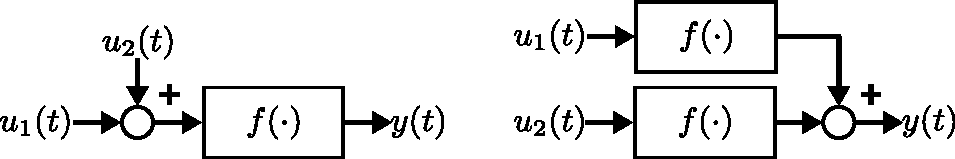
\includegraphics[width=0.8\linewidth]{Abbildungen/Modellbildung/PDF/Summation_Linearitaet.pdf}
	\caption{Vertauschung der Summationstelle bei linearen Übertragungsliedern}
	\label{fig:blockschaltbildsumme}
\end{figure}
%
Die zweite wesentliche Eigenschaft von linearen Systemen ist die \textbf{Homogenität}. Diese beschreibt, dass sich konstante Verstärkungsfaktoren aus einer Funktion ausklammern lassen, ohne, dass sich hierdurch deren Wirkung auf den Systemausgang verändern \eqref{eq:homogen}. 
%
\begin{equation}
y(t) = f\left(ku_{1}(t)\right)=kf\left(u_{1}(t)\right)\label{eq:homogen}
\end{equation}
%
Es ist möglich diesen Zusammenhang wieder in einem Blockschaltbid darzustellen (Abbildung~\ref{fig:blockschaltbildhomogen}). 
%
\begin{figure}[h]
	\centering
	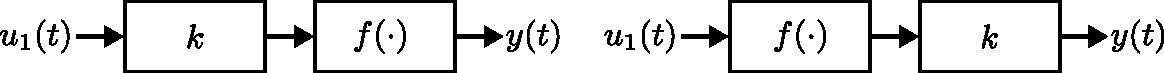
\includegraphics[width=0.9\linewidth]{Abbildungen/Modellbildung/PDF/Homogenitaet.pdf}
	\caption{Vertauschung der konstanten Verstärkungsfaktoren bei linearen Übertragungsliedern}
	\label{fig:blockschaltbildhomogen}
\end{figure}
%
Es lässt sich als Merkregel festhalten: Ist eine Funktion aus einer Summe lineare Übertragungsglieder entstanden, so ist die Funktion selbst wieder linear. 
%
\begin{Aufgaben}{}{}
	\begin{itemize}
		\item \textit{Linearitätsnachweis bei Integratorketten}
		\item \textit{Linearitätsnachweis von MIMO Summationsgliedern}
	\end{itemize}
\end{Aufgaben}
%
\subsubsection{Nichtlineare Übertragunsglieder}
%
Untersucht man nichtlineare Übertragungsglieder so sind die Beiden vorgenannten Eigenschaften nicht vorzufinden. Als einfaches Beispiel lässt sich hier die Multiplikation von zwei Größen darstellen \eqref{eq:multiplikation}
%
\begin{equation}
y(t) = f\left(u_{1}(t),u_{2}(t)\right)=u_{1}(t)\cdot u_{2}(t) \label{eq:multiplikation}
\end{equation}
%
Nehmen wir nun Verstärkungsfaktoren hinzu
%
%
\begin{equation*}
\begin{aligned}
u_{1}(t)&=\hat{k}\hat{u}_{1}(t)+\tilde{k}\tilde{u}_{1}(t)\\
u_{2}(t)&=\hat{k}\hat{u}_{2}(t)+\tilde{k}\tilde{u}_{2}(t)\\
y(t)&=f\left(\hat{k}\,\hat{u}_{1}(t)+\tilde{k}\tilde{u}_{1}(t),\hat{k}\,\hat{u}_{2}(t)+\tilde{k}\tilde{u}_{2}(t)\right)=\left(\hat{k}\,\hat{u}_{1}(t)(t)+\tilde{k}\tilde{u}_{1}(t)\right)\left(\hat{k}\,\hat{u}_{2}(t)+\tilde{k}\tilde{u}_{2}(t)\right)\\
	&= k^{2}\,\hat{u}_{1}(t)\hat{u}_{2}(t)+\tilde{k}^{2}\tilde{u}_{1}(t)\tilde{u}_{2}(t)+\hat{k}\tilde{k}\hat{u}_{1}(t)\tilde{u}_{2}(t)+\hat{k}\tilde{k}\tilde{u}_{1}(t)\hat{u}_{2}(t)\\
\end{aligned}
\end{equation*}
%
wird die Homogenitätsbedingung in diesem Fall nicht erfüllt. Es kann kein konstanter Verstärkungsfaktor $k$ oder $\tilde{k}$ ausgeklammert werden. Ein weiteres Beispiel stellt eine Kennlinie dar. 
%
\begin{figure}[h]
	\centering
	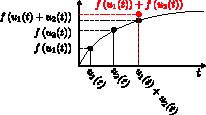
\includegraphics[width=0.6\linewidth]{Abbildungen/Modellbildung/PDF/NichtlinKurve.pdf}
	\caption{Nichtlineare Kennlinie zur Darstellung der Nichtlinearität}
	\label{fig:nichtlinkurve}
\end{figure}
%
Trägt man Werte auf der horizontalen Achse mit gleichem Abstand auf, so ist addiert sich nicht zwingend auch der Funktionswert, wie in Abbildung~\ref{fig:nichtlinkurve} dargestellt. Es ist zu erkennen das die Eigenschaft der Additivität nicht erfüllt ist denn
%
\begin{equation*}
\begin{aligned}
f\left(u_{1}(t)+u_{2}(t)\right)\neq f\left(u_{1}(t)\right)+f\left(u_{2}(t)\right).\\
\end{aligned}
\end{equation*}
%
Grundsätzlich existiert für nichtlineare Systeme in der Regelungstechnik immer noch keine vollständig zusammenhängende Theorie \cite{Adamy09}. Es existieren zudem nicht so zusammenhängende und gut strukturierte Entwurfsverfahren für Regler (mit einigen Ausnahmen).
Die Untersuchung der Stabilität ist ein weiteres Themenfeld, welches in der nichtlinearen Regelungstechnik schwierig zu behandeln ist.
Nichtlineare System werden deshalb in den meisten praktischen Anwendungsfällen durch eine Linearisierung im Arbeitspunkt 'umgewandelt'. Ihr Verhalten kann dann nahe dieses Arbeitspunktes ausreichen gut druch das Ersatzmodell nachgebildet werden und Entwurfsmethoden für lineare Systeme kommen zum Einsatz.
%
\subsection{Zeitinvarianz}
%
Formal lässt sich die Zeitinvarianz eines Systems durch eine Unabhängigkeit der zeitlichen Verschiebung klassifizieren \cite{Foellinger94,Lunze10} \eqref{eq:verschiebungssatz}.
%
\begin{equation}
\begin{aligned}
y(t)&=f\left(u(t)\right)\\
y(t-T)&=f\left(u(t-T)\right)\label{eq:verschiebungssatz}
\end{aligned}
\end{equation}
%
Dies bedeutet, dass sich die Systemantwort eines zeitinvarianten Systems auf einen identischen Eingang (bei gleichem Anfangswert!) immer gleich Verhalten wird, unabhängig davon wann die Anregung durch den Eingang erfolgt.
%
\begin{figure}[h]
	\centering
	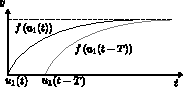
\includegraphics[width=0.55\linewidth]{Abbildungen/Modellbildung/PDF/Zeitinvariant.pdf}
	\caption{Beispielhafte Darstellung des Verschiebungssatzes}
	\label{fig:zeitinvariant}
\end{figure}
%
In Abbildung~\ref{fig:zeitinvariant} ist die Sprungantwort eines zeitinvarianten System dargestellt. Es ist deutlich erkennbar, das sowohl die Kurvenform als auch der Endwert sich nicht unterscheiden. Wenn ein System sowohl linear als  auch zeitinvariant ist, dann spricht man oft von sogenannten 'LZI-System' (lineare und zeitinvariante Systeme) oder Englisch 'LTI-systems' (linear and time-invariant systems). In dieser Vorlesung wird dies die Systemklasse sein, mit der wir uns hauptsächlich beschäftigen.
%
\subsubsection{Beispiele für zeitvariante Systeme}
%
Zeitvariante Systeme sind in der Praxis oft vorzufinden. Ein Beispiel sind zeitlich veränderliche Parameter \cite{Unbehauen08}
\begin{itemize}
	\item Rakete (Massenänderungen des Treibstoffs während des Flugs)
	\item Gleichstrommaschine (temperaturabhängiger Widerstand der Ankerwicklung, welcher sich durch Belastung erwärmt)
\end{itemize}
%
Ein weiteres Beispiel ist das Abtast-Halte-Glied, welches in der zeit-diskreten Regelung zur Wandlug von analogen Signalen genutzt wird. Dieses misst die Regelgröße $y(t)$ in äquidistanten (konstanter Abstand) Zeitpunkten \cite{Foellinger94} und hält den gemessenen Wert als $\overline{y}(\tau)$ für einen konstanten Zeitraum $t_{i}$ fest, wie in Abbildung~\ref{fig:abtastglied} in schwarz dargestellt.
%
\begin{figure}[h]
	\centering
	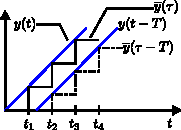
\includegraphics[width=0.4\linewidth]{Abbildungen/Modellbildung/PDF/Abtastglied.pdf}
	\caption{Untersuchung zum Verschiebungssatz bei einem Abtastglied}
	\label{fig:abtastglied}
\end{figure}
%
Dieses Halteglied bereitet somit ein physisches Signal z.B. für einen Microcontroller auf, in dem die Verarbeitung nicht kontinuierlich stattfindet, sondern in diskreten Zeitabständen. \underline{Hinweis:} Das Abtast-Halteglied misst und speichert den kontinuierlichen Wert (Abbildung~\ref{fig:abtastglied} in blau) bis zum nächsten Abtastzeitpunkt $t$ und übernimmt dann den Neuen gemessenen. Diese Glied ist somit zwar linear aber nicht zeitinvariant.
%
%
\begin{Aufgaben}{}{}
	\begin{itemize}
		\item \textit{PWM Stromregelung Gleichstromsteller}
	\end{itemize}
\end{Aufgaben}
%
\subsection{Kausalität}
%
Die Kausalität eines Systems beschreibt, das Eingangsgrößen zum aktuellen Zeitpunkt bspw. $t=0$ den Ausgang nur für zukünftige Zeitpunkte beeinflussen können \cite{Lunze10}. Praktische Systeme sind immer kausal, weshalb diese Eigenschaft in der Vorlesung nicht weiter behandelt werden soll. 
%
%############################################################################
\section{Beschreibung lineare Systeme im Zeitbereich}
%############################################################################
%
%############################################################################
\subsection{Beschreibung lineare Systeme durch Differenzialgleichungen}
%############################################################################
%
Ob ein System durch ein Blockschaltbild oder eine Differentialgleichung dargestellt wird ist grundsätzlich gleichwertig \cite{Ament17}. In der Regel macht sich die Modellbildung die physikalischen Gesetzmäßigkeiten zu nutze und leitet aus ihnen die mathematischen Differenzialgleichungen ab, welche das untersuchte technische System beschreiben. Im folgenden sind die physikalischen Prinzipien, welche für die meisten Systeme ausreichend sind, genannt \cite{Ament17}
\begin{itemize}
	\item Mechanik: also Newtonsche Bewegungseichungen.
	\item Elektrische Systeme: Sätze von Kirchhoff, Strom-Spannungsbeziehung elektrischer Bauteile.
	\item Chemie und Biologie: Bilanzgleichungen für Volumen, Stoff, Massen.
	\item Thermodynamik: Temperatur, Innere Energie, Kreisprozesse
\end{itemize}
%
Formuliert man diese nun zusammen mit deren zeitlichen oder räumlichen Beziehungen zueinander, erhält man die beschreibenden Differenzialgleichungen des Systems.
%
%############################################################################
\subsubsection{Aufstellen und lösen der linearen Differenzialgleichung}
%############################################################################
%
Das Aufstellen und Lösen von Differenzialgleichungen wurde in anderen Grundlagenvorlesungen bereits behandelt, soll hier aber der Vollständigkeit halber nochmals in kurzer Form aufgezeigt werden. Zunächst gehen wir von einer allgemeinen linearen Differenzialgleichung (LDGL) mit konstanten Koeffizienten aus. Diese stellen sich in dieser Vorlesung in folgender Form dar (vgl. Gleichung~\ref{eq:lindgl})
%
\begin{equation}
\begin{aligned}
a_{n}\frac{\text{d}^{n}y}{\text{d}t^{n}}+&a_{n-1}\frac{\text{d}^{n-1}y}{\text{d}t^{n-1}}+\cdots+a_{1}\frac{\text{d}y}{\text{d}t}+a_{0}y=\\
&b_{q}\frac{\text{d}^{q}u}{\text{d}t^{q}}+b_{q-1}\frac{\text{d}^{q-1}u}{\text{d}t^{q-1}}+\cdots+b_{1}\frac{\text{d}u}{\text{d}t}+b_{0}u\label{eq:lindgl}
\end{aligned}
\end{equation}
%
Mit ${a_{0},\dots,a_{n}}$ die konstanten Koeffizienten der linken Seite (Ausgang) und ${b_{0},\dots,b_{n}}$ die konstanten Koeffizienten der rechten Seite (Eingang). Die Variablen $q$ und $n$ stellen jeweils die Höhe der Ableitungen dar. Für diese (LDGL) müssen wir nun, um die homogene Lösung (Eigendynamik oder Eigenbewegung) zu finden, die rechte Seite zu null setzten. Die rechte Seite beschreibt den Eingang auf das System bzw. die Anregung von Außen. 
%
\begin{equation}
\begin{aligned}
&a_{n}\frac{\text{d}^{n}y}{\text{d}t^{n}}+a_{n-1}\frac{\text{d}^{n-1}y}{\text{d}t^{n-1}}+\cdots+a_{1}\frac{\text{d}y}{\text{d}t}+a_{0}y=0 \label{eq:homdgl}
\end{aligned}
\end{equation}
%
Um die LDGL zu lösen wird die charakteristische Gleichung aufgestellt und deren Wurzeln bestimmt. Dabei gilt die Regel: $\frac{\text{d}^{n}y}{\text{d}t^{n}}=\lambda^{n}$. Beim letzten Element setzt man folglich $\frac{\text{d}^{0}y}{\text{d}t^{0}}=1$ (wenn auch mathematisch nicht vollständig korrekt, ist es so leicht zu merken).
%
\begin{equation}
\begin{aligned}
&a_{n}\lambda^{n}+a_{n-1}\lambda^{n-1}+\cdots+a_{1}\lambda+a_{0}=0 \label{eq:characterrischegl}
\end{aligned}
\end{equation}
%
Anschließend wird die Lösung des Polynoms \eqref{eq:characterrischegl} ermittelt. Diese Lösung kann man bei Polynomen mit $n=3$ oder $n<3$ per Hand bestimmen, jedoch werden in der Praxis auch hier meist numerische Verfahren genutzt \cite{Lunze10} \cite{Bruen21}, um die Wurzeln zu bestimmen. Wenn die Wurzeln bestimmt wurden, werden Ansatzfunktionen genutzt, um eine Zeitfunktion für die homogene Lösung zu ermitteln. Falls alle Lösungen $\lambda_{k}=\delta_{k}$ reellwertig sind und nicht doppelt $\delta_{k}\neq\delta_{k+1}$ vorkommen, wird eine Summe aus Exponentialfunktionen genutzt.
%
\begin{equation}
\begin{aligned}
&y_{\text{hom}}(t)=\sum_{k=1}^{N}c_{k}e^{\delta_{k}t}\label{eq:dglloesungreel}
\end{aligned}
\end{equation}
%
Falls es sich um ein schwingungsfähiges System handelt, d.h. es existieren Lösungen für die Wurzeln in Form von $\lambda_{k}=\delta_{k}\pm j\omega_{k}$, wobei $j$ die imaginäre Einheit ist, muss dieser schwingungsfähige Anteil in der Lösung berücksichtigt werden.
%
\begin{equation}
\begin{aligned}
&y_{\text{hom}}(t)=\sum_{k=1}^{N}c_{k}e^{\delta_{k}t}+\sum_{l=1}^{L}e^{\delta_{l}t}\left[c_{1,l}\cos(\omega_{l}t)+c_{2,l}\sin(\omega_{l}t)\right]\label{eq:dglloesungkomplex}
\end{aligned}
\end{equation}
%
%Durch einsetzten der Lösung in Gleichung~\ref{eq:characterrischegl} lassen sich über Koeffizientenvergleich, die Vorfaktoren $c_{k}, c_{l} \forall k,l \in N,L$ in Gleichung~\ref{eq:dglloesungreel} und \ref{eq:dglloesungkomplex} bestimmen.\\

Der zweite Schritt beinhaltet das Auffinden der partikulären Lösung, welche je nach Eingangssignal einen anderen Ansatz besitzt. Eine gute Zusammenfassung verschiedener Ansätze ist in \cite{Furlan08,Gangster03} zu finden. Die wichtigsten Ansätze für die Regelungstechnik sind:
%
\begin{equation}
\begin{aligned}
&u(t) = A, &&\text{Ansatz} \rightarrow y_{\text{part}}(t) = B\\
&u(t) = t^{m}, &&\text{Ansatz} \rightarrow y_{\text{part}}(t) = A_{0}+A_{1}t+\ldots+A_{m}t^{m}\\
&u(t) = A\sin(\omega t), &&\text{Ansatz} \rightarrow y_{\text{part}}(t) = C\sin(\omega t)+D\cos(\omega t)
\end{aligned}
\end{equation}
%
Nachdem der partikuläre Lösungsansatz auswählt wurde, wird dieser in Gleichung~\ref{eq:lindgl} eingesetzt (Ableitungen beachten!) und durch Koeffizientenvergleich die Vorfaktoren ermittelt. Die allgemeine Lösung der Differenzialgleichung ergibt sich aus der Summe von homogener und partikulärer Lösung.
%
\begin{equation}
\begin{aligned}
&y(t)=y_{\text{hom}}(t)+y_{\text{part}}(t)
\end{aligned}
\end{equation}
%
Um die allgemeine Lösung der DGL nun zu bestimmen, müssen Anfangswerte oder allgemein Randwerte der DGL bekannt sein. Dies könnte z.B. die Anfangsauslegung eines Systems sein. Anfangswerte werden benötigt, um die konstanten Koeffizienten der allgemeinen Lösung des homogenen Anteils zu errechnen. Durch Einsetzten der Anfangswerte lassen sich diese wieder durch einen Koeffizientenvergleich bestimmen.
%
Zusammengefasst ergeben sich für die Vorgehensweise beim lösen der DGL:
\begin{itemize}
	\item Auffinden der freien Bewegung (homogene Lösung)
	\item Bestimmung der erzwungenen Bewegung (partikuläre Lösung)
	\item Aufstellen der allgemeinen Lösung
	\item Lösungen des Anfangswertproblems 
\end{itemize}
%
\begin{Aufgaben}{}{}
	\begin{itemize}
		\item \textit{Beispielhafte Lösung der DGL eines mechanischen Systems 2ter-Ordnung}
	\end{itemize}
\end{Aufgaben}
%
%%############################################################################
%\subsubsection{Beispielhafte Lösung eines mechanischen Systems}
%%############################################################################
%%
%Beispielhaft soll hier ein mechanisches System bestehend aus Masse, Dämpfer und einer Feder beschrieben werden, wie in Abbildung~\ref{fig:federmassedaempfer} dargestellt. Dieses System lässt sich als lineare Differentialgleichung zweiter Ordnung beschreiben und für den homogenen Fall folgendermaßen aufstellen \eqref{eq:massedgl}:
%%
%\begin{equation*}
%\begin{aligned}
%m\cdot \frac{\text{d}^{2}x(t)}{\text{d}t^{2}} + d\cdot \frac{\text{d}x(t)}{\text{d}t} + c x(t)=F_{g}\cdot\sin(t)\label{eq:massedgl}
%\end{aligned}
%\end{equation*}
%%
%Um diese LDGL zu lösen nehmen wir zunächst an, dass es sich um ein schwingungsfähiges System handelt, d.h. wir haben eine Lösung der charakteristischen Gleichung der Form $s_{k}=\delta_{k}\pm j\omega_{k}$. Diese setzten wir ein und bekommen
%%
%\begin{equation*}
%\begin{aligned}
%&x_{\text{hom}}(t)=e^{\delta_{l}t}\left[c_{1,l}\cos(\omega_{e}t)+c_{2,l}\sin(\omega_{e}t)\right]
%\end{aligned}
%\end{equation*}
%%
%Die beiden Faktoren $\delta$ und $\omega_{\text{e}}$ erhalten wir aus der Lösung der charakteristischen Gleichung:
%%
%\begin{equation*}
%\begin{aligned}
%&\lambda^{2}+\frac{d}{m}\lambda+\frac{c}{m}=0\\
%&\lambda_{1,2} = \underbrace{-\frac{d}{2m}}_{\delta}\pm \underbrace{\sqrt{\left(\frac{d}{2m}\right)^{2}-\frac{c}{m}}}_{\omega_{\text{e}}}
%\end{aligned}
%\end{equation*}
%%
%Die partikuläre Lösung ergibt sich unter Annahme eines Einheitssprung als Eingang allgemein zu 
%%
%\begin{equation*}
%\begin{aligned}
%%x_{\text{part}}(t)&=\sum_{k=1}^{N}c_{k}(t)x_{k}(t)\\
%x_{\text{part}}(t)&=1
%\end{aligned}
%\end{equation*}
%%
%\eqref{eq:dglloesung} zu
%%
%\begin{equation*}
%\begin{aligned}
%x(t)&=K\left[1 -\frac{1}{\sqrt{1-D^{2}}}\cdot e^{-D\omega_{0}t}\cdot\sin\left(\omega_{e}t+\text{arcos}(D)\right)\right]\\
%&\omega_{e} = \omega_{0}\sqrt{1-D^{2}}
%\end{aligned}
%\end{equation*}
%%
%Das durch diese Differenzialgleichung beschriebene Verhalten wird in Abbildung~\ref{fig:federmassedaempfer} für die Auslenkung um eine Gleichgewichtslage dargestellt. 
%%
%\begin{figure}[h]
%	\centering
%	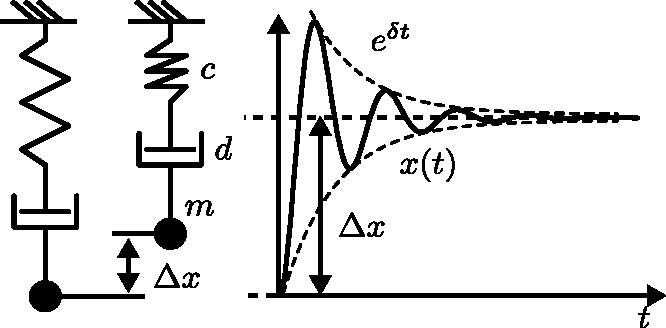
\includegraphics[width=0.65\linewidth]{Abbildungen/Modellbildung/PDF/MasseFederDaempfer.pdf}
%	\caption{Feder, Masse, Dämpfer System und dessen Verhalten bei Auslenkung um eine Gleichgewichtslage}
%	\label{fig:federmassedaempfer}
%\end{figure}  
%%
%############################################################################
\subsubsection{Gewichtsfunktion und Faltung}
%############################################################################
%
Im vorherigen Beispiel haben wir die Auffindung der allgemeinen Lösung einer linearen Differenzialgleichung für ein mechanisches Teilsystem aufgezeigt. Es existiert im Grunde hierfür auch eine kompaktere Schreibweise, denn ein System kann durch eine Lösung der allgemeinen DGL dargestellt werden, welche sich für verschwindende Anfangswerte $y(0)=0$ ergibt. Durch den Anfangswert 0 ist das System in Ruhe und wird nur durch die Anregung eines Eingangssignals aus der Ruhelage ausgelenkt. Das sogenannte Übertragungsverhalten klassifiziert ein dynamisches Systems. Dies bedeutet, dass das System bei verschwindenden Anfangsbedingungen durch sein Ein- Ausgangsverhalten eindeutig beschrieben wird. Die sich ergebende Zeitfunktion wird dann als Gewichtsfunktion $g(t)$ eines dynamischen Systems bezeichnet. Das Systemverhalten auf ein Eingangssignal ergibt sich durch die Berechnung des folgenden Integrals. 
%
\begin{equation}
\begin{aligned}
&y(t)=\int_{0}^{t_{0}}g(t)u(t_{0}-t)\text{d}t\label{eq:faltung}
\end{aligned}
\end{equation}
%
Das Integral \eqref{eq:faltung} wird auch als Faltungsintegral bezeichnet. Die Gewichtsfunktion gibt an, wie stark ein vergangener Wert des Eingangs $u(t_{0}-t)$ durch das Systemverhalten (beschrieben durch $g(t)$) gewichtet wird und somit auf den Ausgang $y(t)$ wirkt. Diese Beschreibung wird in der Literatur auch in folgender Weise dargestellt:
%
\begin{equation}
\begin{aligned}
&y(t)=g(t)*u(t)
\end{aligned}
\end{equation}
%
Grundsätzlich kann man mit dieser Formulierung die Systemantwort eines dynamischen Systems für beliebige Eingangssignale berechnen. Jedoch ist diese Schreibweise trotz allem sehr abstrakt und soll nachfolgend konkretisiert werden. 
%
%############################################################################
\subsubsection{Einheitssprung und Sprungantwort}
%############################################################################
%
In der Regelungstechnik wird zur Anregung des Eingangs eines Systems meist der Einheitssprung (auch Heaviside-Funktion genannt) heran gezogen, welcher durch folgende Beziehung beschrieben wird:
%
\begin{equation}
\begin{aligned}
u(t)=\sigma(t)=\begin{cases}
0  & \text{ falls } t < 0 \\
1  & \text{ falls } t \ge 0 \\
\end{cases}& \label{eq:einheitssprung}
\end{aligned}
\end{equation}
%
Die Sprungantwort $h(t)$ eines Systems beschreibt die Antwort des jeweiligen Systems auf einen Einheitssprung
%
\begin{equation}
\begin{aligned}
&h(t)=\int_{0}^{t_{0}}g(t)\underbrace{\sigma(t_{0}-t)}_{=1}\text{d}t\\
&h(t)=\int_{0}^{t_{0}}g(t)\text{d}t \label{eq:sprungantwort}
\end{aligned}
\end{equation}
%
Somit ist die Sprungantwort $h(t)$ das Integral der Gewichtsfunktion $g(t)$. Dies stellt zusammen mit der Impulsantwort einen wichtigen Zusammenhang in der Regelungstechnik dar. Die Impulsantwort ist definiert als die Antwort des Systems auf einen Einheitsimpuls und wird direkt durch die Gewichtsfunktion $g(t)$ beschrieben. In Abbildung~\ref{fig:federmassedaempfer} wird die Sprungantwort exemplarisch für ein mechanisches System angegeben.
%
Ausgehend von diesen Vorbetrachtungen ist es möglich das dynamische System in einem Zustandsraummodell und Übergangsfunktion (Zeitbereich) oder als Übertragungsfunktion (Frequenzbereich) zu formulieren. Die Zeitbereichsdarstellung bietet für die Regelungstechnik gewisse Vorzüge, soll aber hier aus Zeitgründen nicht weiter betrachtet werden. 
%
\begin{figure}[h]
	\centering
	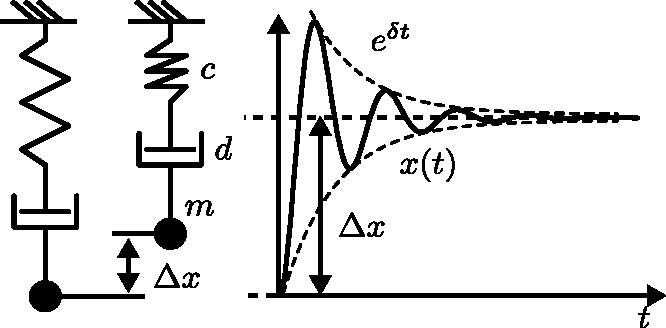
\includegraphics[width=0.65\linewidth]{Abbildungen/Modellbildung/PDF/MasseFederDaempfer.pdf}
	\caption{Feder, Masse, Dämpfer System und dessen Verhalten bei Auslenkung um eine Gleichgewichtslage}
	\label{fig:federmassedaempfer}
\end{figure}  
%
%############################################################################
\section{Beschreibung lineare Systeme im Frequenzbereich}
%############################################################################
%
%############################################################################
\subsection{Fourier Reihenentwicklung}
%############################################################################
%
Die Zerlegung von Funktionen in ihre unterschiedlichen Bestandteile und die Darstellung als Summe dieser Bestandteile sind ein gängiges Mittel, um komplizierte Funktionen zu vereinfachen. Eine Besonderheit stellen periodische Zeitfunktionen dar. Diese können durch eine Summe von unendlich vielen Sinus- und Cosinusfunktionen dargestellt werden, da diese ebenfalls periodisch sind. Diese Aussage kennen wir von den sogenannten
Fourier-Reihen \cite{Furlan08}.
%
\begin{equation}
\begin{aligned}
u(t)&=\frac{A_{0}}{2}+\sum_{k=1}^{\infty}A_{k}\cos(k\omega_{0}t)+\sum_{k=1}^{\infty}B_{k}\sin(k\omega_{0}t)
\end{aligned}
\end{equation}
%
\begin{figure}[h]
	\centering
	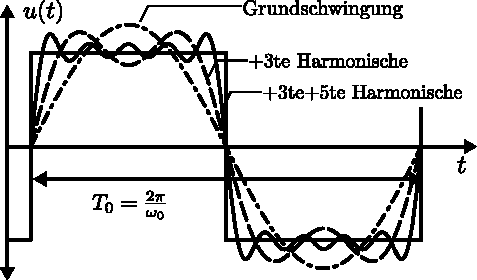
\includegraphics[width=0.675\linewidth]{Abbildungen/Modellbildung/PDF/Fourierreihe.pdf}
	\caption{Annäherung einer periodischen Rechteckfunktion mittels Fourierreihen, in Anlehnung an \cite{Lunze10}}
	\label{fig:fourierreihe}
\end{figure}  
%
Beispielsweise kann hierdurch eine periodische Rechteckfunktion $u(t)$ durch eine Summe von Sinustermen dargestellt werden (Abbildung~\ref{fig:fourierreihe}). Die Faktoren $A_{0}$,$A_{k}$ und $B_{k}$ erhält man aus den Integralbeziehungen
%
\begin{equation*}
\begin{aligned}
A_{0}&=\frac{2}{T_{0}}\int_{0}^{T_{0}}u(t)\text{d}t \quad\\
A_{k}&=\frac{2}{T_{0}}\int_{0}^{T_{0}}u(t)          \cos(k\omega_{0}t)\text{d}t \quad (k=1,2,\ldots)\\
B_{k}&=\frac{2}{T_{0}}\int_{0}^{T_{0}}u(t)\sin(k\omega_{0}t)\text{d}t \quad (k=1,2,\ldots)
\end{aligned}
\end{equation*} 
%
\begin{simulation}{}{}
	\begin{itemize}
		\item \textit{Fourierreihenentwicklung einer Sägezahnfunktion}
		\item \textit{Fourierreihenentwicklung einer Rechteckschwingung}
	\end{itemize}
\end{simulation}
%
Da die Zeitfunktionen sich in diesem Fall nur in Frequenz und Amplitude unterscheiden, können Sie auch als diskretes Frequenzspektrum dargestellt werden, ohne das Informationen verloren gehen (vgl. Abbildung~\ref{fig:spektrumdiskret}). Hieraus ergibt sich die Bezeichnung: \glqq{}im Frequenzbereich beschreiben\grqq{}. Hierbei können entweder die Amplituden der jeweiligen sinus- und cosinus-Terme in ein Diagramm eingetragen werden, oder es wird eine Darstellung aus Betrag und Phase gewählt. Im Folgenden wird die Darstellung mittels Betrag und Phase angegeben, da sie für die weitere Vorlesung wesentlich interessanter ist.
%
\begin{figure}[h]
	\centering
	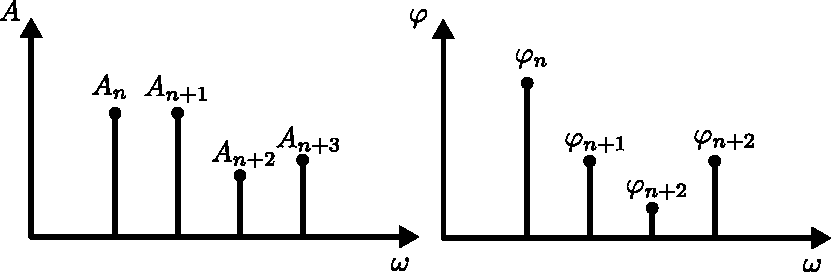
\includegraphics[width=0.75\linewidth]{Abbildungen/Modellbildung/PDF/DiskretesSpektrum.pdf}
	\caption{Darstellung der sinus- und cosinus-Funktionen der Fourierreihe mittels Betrag und Phase als diskretes Spektrum}
	\label{fig:spektrumdiskret}
\end{figure}
%
Eine kompaktere Darstellung im Gegensatz zur Schreibweise mittels getrennter sinus- und cosinus Funktionen, kann durch den Zusammenhang 
%
\begin{equation*}
\begin{aligned}
e^{-jk\omega_{0}t}&=\cos(k\omega_{0}t)-j\sin(k\omega_{0}t)
\end{aligned}
\end{equation*} 
%
erreicht werden. Die Berechnung der Koeffizienten wird durch diese Formulierung in komplexer Schreibweise dargestellt
%
\begin{equation*}
\begin{aligned}
F_{k}&=\frac{1}{T_{0}}\int_{t_{0}}^{t_{0}+T_{0}}u(t)e^{-jk\omega_{0}t}\text{d}t \quad (k=0,\pm 1,\pm 2,\ldots)
\end{aligned}
\end{equation*} 
%
muss aber nach der Berechnung noch umgewandelt werden in Betrag und Phase, was der vorherigen Darstellung in Abbildung~\ref{fig:spektrumdiskret} entspricht. 
%
%############################################################################
\subsection{Fouriertransformation}
%############################################################################
%
Werden nun nichtperiodische Funktionen betrachtet (z.B. Sprung, Impuls), welche quasi eine unendliche Periode $T_{0}$ haben, kann die Funktion nicht mehr durch diskrete Frequenzen und Phasenlagen beschrieben werden. Die einzelnen diskreten Fourierkoeffizienten bei periodischen Signalen rücken bei immer größer werdender Periode immer näher zusammen und bilden schlussendlich beim Übergang zu einer unendlichen Periode eine kontinuierliche Funktion. Diese Funktion wird auch als die Fouriertransformierte des jeweiligen Zeitsignals $u(t)$ bezeichnet und beschreibt die Frequenzanteile bezogen auf sinus- und cosinusförmige Signale.
%
\begin{equation*}
\begin{aligned}
F(j\omega)&=\int_{-\infty}^{\infty}u(t)e^{-j\omega t}\text{d}t 
\end{aligned}
\end{equation*} 
%
Neben Zeitfunktionen lassen sich auch Differentialgleichungen unter gewissen Randbedingungen mittels Fouriertransformation in eine Darstellung im Frequenzbereich transformieren. Dies ist eine der ursprünglichen Intentionen des Erfinders und wurde genutzt, um Lösungen für partielle Differentialgleichungen in der Wärmetheorie zu untersuchen. Die Fouriertransformation führt im wesentlichen dazu, dass ein Differential- in einen algebraischen Zusammenhang überführt wird. 
%
%\begin{Aufgaben}{}{}
%	\begin{itemize}
%		\item \textit{Fouriertransformation Beispiele mittels Tabelle und vollständig}
%	\end{itemize}
%\end{Aufgaben}
%
%##################################################
\subsection{Der Frequenzgang eines LZI-Übertragungsgliedes} 
%##################################################
%
%############################################################################
\subsubsection{Allgemeine Betrachtung des Frequenzgang}
%############################################################################
%
Der Frequenzgang $G(j\omega)$ eines LZI-Systems beschreibt wie sich der Systemausgang $y(t)$ auf eine Anregung mit einer Sinusfunktion am Eingang $u(t)$ verhält. 
%
\begin{figure}[h]
	\centering
	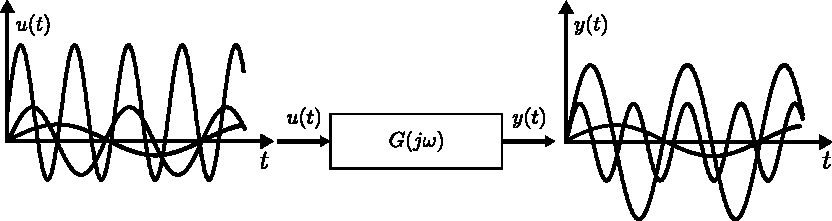
\includegraphics[width=1\linewidth]{Abbildungen/Modellbildung/PDF/Frequenzgang.pdf}
	\caption{Prinzipdarstellung des Frequenzgangs von LZI-Gliedern, in Anlehnung an \cite{Lunze10}}
	\label{fig:frequenzgang}
\end{figure}  
%
Wichtig ist zu vermerken, dass keine Anfangswerte berücksichtigt werden und das, dass Systemverhalten nur für den stationären Fall abgebildet wird (Ausgleichsvorgänge sind abgeklungen). Der Zusammenhang zur Fouriertransformierten entsteht, wenn die Berechnung aus \eqref{eq:faltung} mit sinusförmigen Eingangsfunktionen $u(t)$ berechnet wird (ohne Herleitung). Der Frequenzgang eines Systems ist somit die Fouriertransformierte der Gewichtsfunktion.
%
\begin{equation*}
\begin{aligned}
G(j\omega)&=\mathcal{F}\{g(t)\}
\end{aligned}
\end{equation*}
%
Der Frequenzgang ist in der Regelungstechnik einer der wichtigsten Werkzeuge, da er die Grundlage vieler Analysen bildet. Er lässt sich zudem messtechnisch ermitteln, da er durch Zeitfunktionen am Eingang und der Messung der Systemantworten am Ausgang bestimmt werden kann. Das Ausgangssignal ist lediglich in Amplitude und Phasenlage unterschiedlich zum Eingang, jedoch ändert sich nicht die Frequenz. In der komplexen Darstellung lässt sich der Frequenzgang wie folgt beschreiben
%
\begin{equation*}
\begin{aligned}
G(j\omega)&=\frac{Y(j\omega)}{U(j\omega)}\\
&=\frac{\hat{y}(j\omega)e^{j\omega}e^{j\varphi_{y}(j\omega)}}{\hat{u}(j\omega)e^{j\omega}e^{j\varphi_{u}}}\\
&=\frac{\hat{y}(j\omega)}{\hat{u}(j\omega)}e^{j\varphi_{yu}(j\omega)}
\end{aligned}
\end{equation*}
%
Jedoch gibt es auch die Möglichkeit den Frequenzgang in Betrag und Phase darzustellen
%
\begin{equation*}
\begin{aligned}
G(j\omega)&=\Re\{G(j\omega)\}+j\Im\{G(j\omega)\}\\
\left|G(j\omega)\right|&=\sqrt{\left(\Re\{G(j\omega)\}\right)^{2}+\left(\Im\{G(j\omega)\}\right)^{2}}\\
\angle G(j\omega)&=\arctan\left(\frac{\Im\{G(j\omega)\}}{\Re\{G(j\omega)\}}\right)
\end{aligned}
\end{equation*}
%
Zwei Darstellungen beschreiben den Frequenzgang grafisch.
%
\begin{itemize}
	\item Ortskurve, welche ein Zeigerdiagramm in der komplexen Ebene mit $\omega$ als Parameter darstellt.
	\item Bodediagramm oder Frequenzkennliniendiagramm in logarithmischer Darstellung.
\end{itemize}
%
\subsubsection{Die Ortskurve eins LZI-Übertragungsgliedes}
%
Die Ortskurve stellt den Amplituden- und Phasengang des Frequenzgangs in der komplexen Ebene mit $\omega$ als Parameter dar. Dieser Zusammenhang ist in Abbildung~\ref{fig:Ortskurve} dargestellt.
%
\begin{figure}[h!]
	\centering
	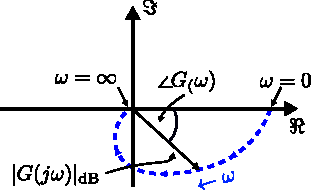
\includegraphics[width=0.45\linewidth]{Abbildungen/Modellbildung/PDF/Ortskurve.pdf}
	\caption{Ortskurve eines dynamischen System}
	\label{fig:Ortskurve}
\end{figure}
%
Über die Grenzwerte im Frequenzbereich lassen sich die Funktionen im Diagramm zeichnen. Nehmen wir das IT$_{1}$-Glied als Beispiel (aus \cite{Lunze10}), so erhalten wir für den Frequenzgang
%
\begin{equation*}
\begin{aligned}
%
G(j\omega)&=\frac{1}{j\omega T_{\text{I}}\left(j \omega T_{1}+1\right)}\\
%
&=\frac{1}{\left(-\omega^{2}T_{\text{I}}T_{1}+j\omega T_{\text{I}}\right)}\cdot\frac{\left(-\omega^{2}T_{\text{I}}T_{1}-j\omega T_{\text{I}}\right)}{\left(-\omega^{2}T_{\text{I}}T_{1}-j\omega T_{\text{I}}\right)}\\
%
&=\frac{-\omega T_{1}-j}{\omega T_{\text{I}}\left(\omega^{2}T^{2}_{1}+1\right)}\\
%
&=\frac{-T_{1}}{T_{\text{I}}\left(\omega^{2}T^{2}_{1}+1\right)}-j\frac{1}{\omega T_{\text{I}}\left(\omega^{2}T^{2}_{1}+1\right)}\\
%
\end{aligned}
\end{equation*} 
%
Hieraus lassen sich nun der Anfangs- und Endwert aus der Grenzwertbetrachtung
%
\begin{equation*}
\begin{aligned}
%
\lim\limits_{\omega\rightarrow \infty}G(j\omega)&=0\\
%
\lim\limits_{\omega\rightarrow 0}\Re\{G(j\omega)\}&=-\frac{T_{1}}{T_{\text{I}}}\\
%
\lim\limits_{\omega\rightarrow 0}\Im\{G(j\omega)\}&=-\infty.
%
\end{aligned}
\end{equation*} 
%
ermitteln und nachfolgend die Ortskurve zeichnen (siehe Abbildung~\ref{fig:OrtskurveIT1}).
%
\begin{figure}[h!]
	\centering
	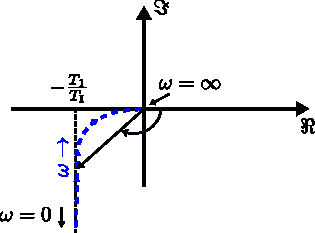
\includegraphics[width=0.50\linewidth]{Abbildungen/Systemanalyse/PDF/OrtskurveIT1.pdf}
	\caption{Ortskurve des IT$_{1}$-Gliedes}
	\label{fig:OrtskurveIT1}
\end{figure}
%
Es soll hier zudem erwähnt werden, dass der Verlauf der Amplitude und der Phase von $\omega=0$ bis $\omega=\infty$ auch durch die bekannten Verfahren der Frequenzkennlinie berechnet werden kann. 
%
\subsubsection{Die Frequenzkennlinien oder Bodediagramm eins LZI-Übertragungsgliedes \cite{Lunze10}}
%
Die Darstellung in der Ortskurve ist nicht die einzige Möglichkeit, um das Verhalten eines dynamischen Systems im Frequenzbereich zu analysieren. Allgemein wird diese auch als Frequenzkennlinie (FKL) bezeichnet. Eine sehr allgemeine, aber durchaus recht vollständige Darstellung des Frequenzgang kann durch folgende Beschreibung erreicht werden:
%
\begin{equation*}
\begin{aligned}
%
G(j\omega)=k \underbrace{\cdot \frac{1}{(j\omega)^{q}}}_{\text{I-Glieder}} \cdot \underbrace{\frac{\prod_{i=1}\left(j \omega T_{i}+1\right)}{\prod_{\nu=1}\left(j \omega T_{\nu}+1\right)}}_{\text{PT}_{1}~\text{-Glieder}} 
%
\cdot\underbrace{\frac{\prod_{k=1}\left(\left(\frac{j \omega}{\omega_{0 k}}\right)^{2}+\frac{j \omega}{\omega_{0 k}} 2 d_{k}+1\right)}{\prod_{\mu=1}\left(\left(\frac{j \omega}{\omega_{0 \mu}}\right)^{2}+\frac{j \omega}{\omega_{0 \mu}} 2 d_{\mu}+1\right)}}_{\text{PT}_{2}~\text{-Glieder}} 
%
\cdot \underbrace{e^{-T_{t}j\omega}}_{\text{Totzeit-Glied}} 
%
\end{aligned}
\end{equation*}  
%
gebracht. Durch die Überlagerung dieser Grundglieder lässt sich der Frequenzgang $G(j\omega)$ möglichst genau darstellen. Bedingung hierfür ist jedoch das:
%
\begin{itemize}
	\item $0<d_{k},d_{\mu}<1$: gedämpft aber schwingungsfähig.
	\item $\omega_{0k},\omega_{0\mu},T_{i},T_{\nu},T_{t}>0$: Kausalitätsbedingung.
	\item $k>0$: Gegenkopplungsbedingung.
	\item $q \le 2$: Bedingung für Stabilitätsnachweis über vereinfachtes Nyquistkriterium. 
\end{itemize}
%
Somit ergibt sich, dass $G(j\omega)$ sich aus den Frequenzgängen der Grundglieder und deren Inversen zusammensetzt. Die Rechenregeln hierfür lauten:
%
\begin{equation*}
\begin{aligned}
%
\quad\quad &G(j\omega)=|G(j\omega)|e^{j\varphi},\,\varphi=\angle G(j\omega)\\
%
\end{aligned}
\end{equation*}
%
Die Inversionsregel ergibt sich zu:
%
\begin{equation*}
\begin{aligned}
%
\quad\quad  &G^{-1}(j\omega)=\frac{1}{|G(j\omega)|}e^{-j\varphi}\\
%
&|G^{-1}(j\omega)|=\frac{1}{|G(j\omega)|}.\\
%
\end{aligned}
\end{equation*}
%
Was sich im Amplituden und Phasengang zu:
%
\begin{equation*}
\begin{aligned}
%
&|G^{-1}(j\omega)|_{\text{dB}}=20\lg\left(\frac{1}{|G(j\omega)|}\right)=-20\lg\left(|G(j\omega)|\right)\\
%
&\angle G^{-1}(j\omega) = - \angle G(j\omega)
%
\end{aligned}
\end{equation*}
%
ergibt. Es ist ersichtlich, dass die Inversion zu einer Spiegelung der FKL an der Null-Linie führt ($0_{\text{dB}}$ bzw. $0^{\circ}$).\\ Die Multiplikationsregel hingegen ergibt sich zu:
%
\begin{equation*}
\begin{aligned}
%
\quad\quad &G(j\omega)=G_{1}(j\omega)\cdot G_{2}(j\omega) \cdot\ldots\cdot G_{n}(j\omega)\\
%
&G(j\omega)=|G_{1}(j\omega)|e^{j\varphi_{1}}\cdot|G_{2}(j\omega)|e^{j\varphi_{2}}\cdot \ldots \cdot |G_{n}(j\omega)|e^{j\varphi_{n}}\\
%
&G(j\omega)=\left(|G_{1}(j\omega)|\cdot|G_{2}(j\omega)|\cdot\ldots\cdot|G_{n}(j\omega)\right)e^{j\left(\varphi_{1}+\varphi_{2}+\ldots+\varphi_{n}\right)}\\
%
\end{aligned}
\end{equation*}
%
Was sich im wiederum im Amplituden- bzw. Phasengang zu:
%
\begin{equation*}
\begin{aligned}
%
|G(j\omega)|_{\text{dB}}&=20\lg\left(|G_{1}(j\omega)|\cdot|G_{2}(j\omega)|\cdot\ldots\cdot|G_{n}(j\omega)\right)\\
%
&=20\lg\left(|G_{1}(j\omega)|\right)+20\lg\left(|G_{2}(j\omega)|\right)+\ldots+20\lg\left(|G_{n}(j\omega)|\right)\\
%
\angle G(j\omega) &=\angle G_{1}(j\omega)+\angle G_{2}(j\omega)+\ldots+\angle G_{n}(j\omega)
%
\end{aligned}
\end{equation*}
%
ergibt. Das bedeutet, dass eine Multiplikation der Frequenzgänge eine Addition in der FKL zur Folge hat.\\
\underline{Hinweis:} Eine Multiplikation ist gleichbedeutend mit der Hintereinanderschaltung einzelner Übertragungsglieder im Wirkschaltplan.\\
%
%Das Bodediagramm ist eine graphische Darstellung des Frequenzgang. Hierbei wird der Amplitudengang $\left|G(j\omega)\right|$ und der Phasengang $\angle G(j\omega)$ in zwei getrennte Abbildungen eingetragen. Um größere Frequenzbereiche für $\omega$ einzeichnen zu können, wird der Amplitudengang meist logarithmisch aufgetragen. Dabei gilt der Zusammenhang
%%
%\begin{equation*}
%\begin{aligned}
%\left|G(j\omega)\right|_{\text{dB}}=20 \lg \left|G(j\omega)\right|\\
%\angle G(j\omega)=\text{argmin}\left(G(j\omega)\right)
%\end{aligned}
%\end{equation*}
%
Für den Betrag und die Phase eines PT$_{1}$ Übertragungsgliedes, lassen sich folgende Berechnung schritte aufzeigen.
%
\begin{equation*}
\begin{aligned}
%
G(j\omega)&=\frac{K_{\text{P}}}{T_{1}j\omega+1}=\frac{K_{\text{P}}}{T_{1}j\omega+1}\cdot\frac{-T_{1}j\omega+1}{-T_{1}j\omega+1}=\frac{K_{\text{P}}\left(1-T_{1}j\omega\right)}{T^{2}_{1}\omega^{2}+1}\\
%
|G(j\omega)|_{\text{dB}}&=20\lg|G(j\omega)|=20\lg\left(\frac{K_{\text{p}}}{\sqrt{T^{2}_{1}\omega^{2}+1}}\right)\\
%
&=20\lg\left(K_{\text{p}}\right)-20\lg\left(\sqrt{T_{1}^{2}\omega^{2}+1}\right)\\
%
\angle G(j\omega)&=\arctan\left(\frac{-\frac{K_{\text{p}}\omega T_{1}}{T^{2}_{1}\omega^{2}+1}}{\frac{K_{\text{p}}}{T^{2}_{1}\omega^{2}+1}}\right)=\arctan\left(-\omega T_{1}\right)=-\arctan\left(\omega T_{1}\right)\\
\end{aligned}
\end{equation*}
%
\begin{figure}[ht!]
	%
	\centering
	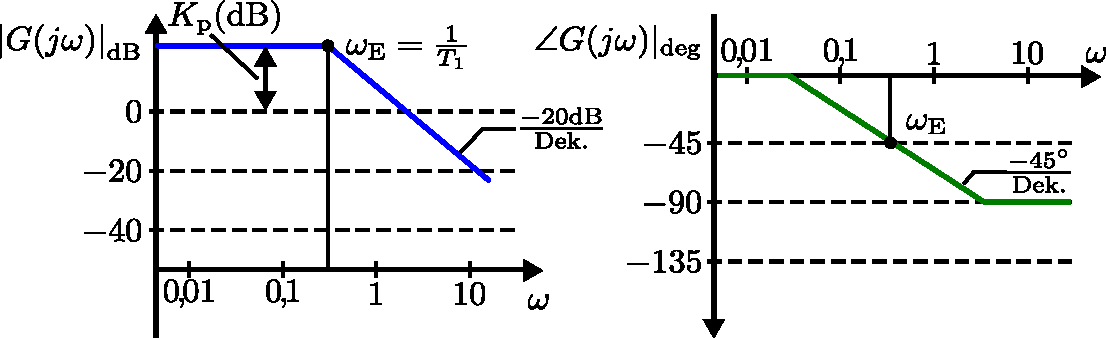
\includegraphics[width=0.9\linewidth]{Abbildungen/Modellbildung/PDF/PT1gliedBode.pdf}
	\caption{Bodediagramm zur Darstellung des Frequenzgangs, exemplarisch für ein dynamisches System}
	\label{fig:bodediagramm}
	%
\end{figure} 
%
Zur grafischen Darstellung wird auf der horizontalen Achse die Frequenz und auf der vertikalen die Amplitude aufgetragen. Die Frequenz wird meist in einer logarithmischen Skala angegeben. D.h. in linearer Unterteilung als $\lg\omega$ oder als Zehnerpotenzen mit $\omega$. 
%
Der Amplitudengang wird in Dezibel gegen die logarithmische Frequenz aufgetragen während der Phasengang unverändert auf der vertikalen Achse gegen die logarithmische Frequenz aufgetragen wird.
Es bietet sich an die beiden Diagramme bei der Konstruktion untereinander zu zeichnen und die Frequenz in gleicher Skalierung aufzutragen. Die vorgenannte Formalen Zusammenhänge sind in Abbildung~\ref{fig:bodediagramm} qualitativ dargestellt. 
%
\newpage
%############################################################################
\subsection{Laplacetransformation}
%############################################################################
%
%Der Frequenzgang ist nicht geeignet, um die Dämpfung eines technischen Systems zu beschreiben bzw. zu analysieren. Dämpfung tritt physikalisch meist durch eine Umwandlung von innerer Energie in Wärme auf. 
Die Laplacetransformation kann als Erweiterung der Fouriertransformationen verstanden werden. Diese Erweiterung ermöglicht es z.B. Differenzialgleichungen über den sogenannten Bildbereich zu lösen (vgl. Abbildung~\ref{fig:laplacetransformation}). Der Bildbereich stellt sämtliche Differentiale aus dem Zeitbereich in algebraischen Gleichungen dar.
%
\begin{figure}[h]
	\centering
	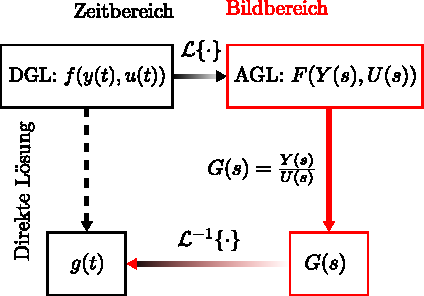
\includegraphics[width=0.55\linewidth]{Abbildungen/Modellbildung/PDF/LaplaceTransformation.pdf}
	\caption{Darstellung der Laplacetransformation zur Lösung von Differenzialgleichungen}
	\label{fig:laplacetransformation}
\end{figure}
%
Nun tritt z.B. beim Feder-Masse-Dämpfer in Abbildung~\ref{fig:federmassedaempfer} eine Dämpfung der Schwingung in Form einer Exponentialfunktion auf, die dafür sorgt, dass die sich ergebende Schwingung abklingt und das System nach einer endlichen (theoretisch unendlichen) Zeit wieder in eine Ruhelage übergeht. Dieses Verhalten, dass sogenannte Übergangsverhalten kann durch den Frequenzgang nicht abgebildet werden. Um diese Eigenschaft eines Systems jedoch trotzdem im Frequenzbereich (Bildbereich) mit all seinen Vorteilen zu erfassen, erweitert die Laplacetransformation \eqref{eq:laplace} den Frequenzbereich der Fouriertransformation um Exponentialfunktionen mit $s=\delta+j\omega$ zu
%
\begin{equation}
\begin{aligned}
F(s)&=\int_{0}^{\infty}f(t)e^{-st}\text{d}t\label{eq:laplace}
\end{aligned}
\end{equation}
%
Zudem ist zu beachten, das die Integral Grenzen nun nur von $0$ bis $\infty$ reichen, da wir annehmen, dass alle nicht periodischen Signale kausal und somit für $t<0$ nicht definiert sind. Das Hauptaugenmerk für die Behandlung in der Regelungstechnik ist, wie bereits oben erwähnt, dass sich mit Hilfe der Beziehung \eqref{eq:laplace} Differentialgleichungen nun durch algebraische Gleichungen darstellen lassen. Hierfür gibt es meist Rechentabellen, welche die wichtigsten Beziehungen zwischen Zeitbereich und Bildbereich darstellen.\\
%
Die Laplace-Transformation hat auch eine grafische Interpretation, denn sie Erweitert das kontinuierliche Spektrum der Fouriertransformation für Signale mit abklingenden e-Funktionen. 
%
%############################################################################
\subsubsection{Übertragungsfunktion}
%############################################################################
%
Die Übertragunsfunktion eines Systems ist die Laplacetransformierte der Gewichtsfunktion \eqref{eq:uebertragungsfunktion}.
%
\begin{equation}
\begin{aligned}
G(s)&=\mathcal{L}\{g(t)\}\label{eq:uebertragungsfunktion}
\end{aligned}
\end{equation}
%
Auch hier ist wieder zu erwähnen, dass keine Anfangswerte berücksichtigt werden, jedoch können Einschwingvorgänge abgebildet werden. Dies ist besonders wichtig, wenn keine sinusförmigen Eingänge auf das System wirken. Der Übergang zurück zum Frequenzgang entsteht, wenn wir eine sinusförmige Anregung an ein System anlegen und alle Einschwingvorgänge abgeklungen sind $t\rightarrow\infty$, oder wenn es im System keine Dämpfung gibt $\delta=0$. 
%
Aus diesem Grund können beide Übertragungseigenschaften zur Analyse von Regelung und Regelstrecke herangezogen werden. Auch die Übertragungsfunktion lässt sich messtechnisch ermitteln, jedoch ist dies meist schwieriger wie im Falle des Frequenzgangs und wird deshalb im späteren Verlauf der Vorlesung nur für einige Spezialfälle behandelt. Die Darstellung der Übertragungsfunktion kann folgendermaßen aussehen: 
%
\begin{equation*}
\begin{aligned}
G(s)&=\frac{Y(s)}{U(s)}\\
&=\frac{\hat{y}(s)e^{j\varphi_{y}(s)}}{\hat{u}(s)e^{j\varphi_{u}(s)}}\\
&=\frac{\hat{y}(s)}{\hat{u}(s)}e^{j\varphi_{y}(s)-\varphi_{u}(s)}
\end{aligned}
\end{equation*}
%
Jedoch gibt es auch die Möglichkeit der Übertragungsfunktion in Betrag und Phase darzustellen
%
\begin{equation*}
\begin{aligned}
G(s)&=\Re\{G(s)\}+j\Im\{G(s)\}\\
\left|G(s)\right|&=\sqrt{\left(\Re\{G(s)\}\right)^{2}+\left(\Im\{G(s)\}\right)^{2}}\\
\angle G(s)&=\arctan\left(\frac{\Im\{G(s)\}}{\Re\{G(s)\}}\right)
\end{aligned}
\end{equation*}
%
Die Übertragungsfunktion wird hauptsächlich zur Reglerauslegung verwendet.
%
\begin{itemize}
	\item Pol-Nullstellen Diagramm $\rightarrow$ Analyse der Pollage und Stabilitätsuntersuchung der offenen Wirkungskette.
	\item Wurzelortsurve $\rightarrow$ Regelerauslegung anhand der Pollage bei veränderlicher Verstärkung
\end{itemize}
%
%############################################################################
\subsubsection{Allgemeine Berechnung der Übertragungsfunktion aus der Differentialgleichung}
%############################################################################
%
Mittels der Laplacetransformation lassen sich gewöhnliche lineare Differenzialgleichungen in algebraische Gleichungen 'umwandeln'. 
\begin{itemize}
\item Schritt 1: Aufstellen der Differenzialgleichung.
%
\begin{equation*}
\begin{aligned}
a_{n}\frac{\text{d}^{n}y}{\text{d}t^{n}}+&a_{n-1}\frac{\text{d}^{n-1}y}{\text{d}t^{n-1}}+\cdots+a_{1}\frac{\text{d}y}{\text{d}t}+a_{0}y=\\
&b_{q}\frac{\text{d}^{q}u}{\text{d}t^{q}}+b_{q-1}\frac{\text{d}^{q-1}u}{\text{d}t^{q-1}}+\cdots+b_{1}\frac{\text{d}u}{\text{d}t}+b_{0}u\\
\end{aligned}
\end{equation*}
%
\item Schritt 2: Transformation in den Bildbereich durch Rechentabelle und Ableitungsregel (Anfangswerte vernachlässigen).
%
\begin{equation*}
\begin{aligned}
a_{n}s^{n}Y(s)+&a_{n-1}s^{n-1}Y(s)+\cdots+a_{1}sY(s)+a_{0}Y(s)=\\
&=b_{q}s^{q}U(s)+b_{q-1}s^{q-1}U(s)+\cdots+b_{1}sU(s)+b_{0}U(s)\\
\end{aligned}
\end{equation*}
%
\item Schritt 3: Ausklammern und umstellen
%
\begin{equation*}
\begin{aligned}
Y(s)&\left(a_{n}s^{n}+a_{n-1}s^{n-1}+\cdots+a_{1}s+a_{0}\right)=\\
&=U(s)\left(b_{q}s^{q}+b_{q-1}s^{q-1}+\cdots+b_{1}s+b_{0}\right)\\
\end{aligned}
\end{equation*}
%
%
\item Schritt 4: Übertragungsfunktion aufstellen
%
\begin{equation*}
\begin{aligned}
G(s)=\frac{b_{q}s^{q}+b_{q-1}s^{q-1}+\cdots+b_{1}s+b_{0}}{a_{n}s^{n}+a_{n-1}s^{n-1}+\cdots+a_{1}s+a_{0}}\\
\end{aligned}
\end{equation*}
%
\end{itemize}
%
%############################################################################
\subsubsection{Beispiel: Feder-Masse-Dämpfer}
%############################################################################
%
Nehmen wir zunächst die Differentialgleichung des Feder-Masse-Dämpfers ohne äußere Anregung
%
\begin{equation*}
\begin{aligned}
m\cdot \frac{\text{d}^{2}x(t)}{\text{d}t^{2}} + d\cdot \frac{\text{d}x(t)}{\text{d}t} + c x(t)=0
\end{aligned}
\end{equation*}
%
so ließe sich durch Anwendung der Laplacetransformation folgender Zusammenhang finden
%
\begin{equation*}
\begin{aligned}
\underbrace{s^{2}X(s)-sx(0)-\frac{\text{d}x(0)}{\text{d}t}}_{s^{2}\mathcal{L}\{f(t)\}-sf(0)-\frac{\text{d}f(0)}{\text{d}t}} + \underbrace{\frac{d}{m}\left(sX(s)-x(0)\right)}_{s\mathcal{L}\{f(t)\}-f(0)} + \frac{c}{m}X(s)=0
\end{aligned}
\end{equation*}
%
Da Anfangswerte vernachlässigt werden, können wir die Gleichung umwandeln in
%
\begin{equation*}
\begin{aligned}
s^{2}X(s) + \frac{d}{m}X(s)s + \frac{c}{m}X(s)=0
\end{aligned}
\end{equation*}
%
Durch Umstellen der Gleichung erhalten wir nun die Übertragungsfunktion des Systems im Laplace Bereich
%
\begin{equation*}
\begin{aligned}
G(s)= \frac{1}{s^{2} + \frac{d}{m}s + \frac{c}{m}}\\
%
\end{aligned}
\end{equation*}
%
Und die Übergangsfunktion durch hinzufügen eines Einheitssprung am Eingang  
%
\begin{equation*}
\begin{aligned}
%
H(s)= \frac{1}{s\left(s^{2} + \frac{d}{m}s + \frac{c}{m}\right)}
%
\end{aligned}
\end{equation*}
%
Abbildung~\ref{fig:federmassedaempfer} stellt die Sprungantwort $h(t)$ des schwingungsfähigen Systems dar. Die Anregung erfolgt in diesem Fall durch eine Auslenkung um die Ruhelage.
%
%############################################################################
\subsection{Pole und Nullstellen der Übertragungsfunktion}
%############################################################################
%
Der Pol- Nullstellenplan ermöglicht die Eigenschaften der Regelstrecke graphisch zu analysieren. Um die Pole und Nullstellen auszurechnen, müssen die Polynome der Übertragungsfunktion 
%
\begin{equation*}
\begin{aligned}
G(s)=\frac{b_{q}s^{q}+b_{q-1}s^{q-1}+\cdots+b_{1}s+b_{0}}{a_{n}s^{n}+a_{n-1}s^{n-1}+\cdots+a_{1}s+a_{0}}\\
\end{aligned}
\end{equation*}
%
in ihre einzelnen Bestandteile zerlegt werden.
%
\begin{equation}
\begin{aligned}
G(s)=k\frac{\left(s-s_{\text{N},1}\right)\left(s-s_{\text{N},2}\right)\ldots\left(s-s_{\text{N},q}\right)}{\left(s-s_{\text{P},1}\right)\left(s-s_{\text{P},2}\right)\ldots\left(s-s_{\text{P},n}\right)}=k\frac{\prod_{i=1}^{q}\left(s-s_{\text{N},i}\right)}{\prod_{i=1}^{n}\left(s-s_{\text{P},i}\right)}\label{eq:polnullstellenform}\\
\end{aligned}
\end{equation}
%
Jeder dieser Pole und Nullstellen, welche Beispielsweise durch Partialbruchzerlegung errechnet wurden, kann nun in das Pol- Nullstellendiagramm Abbildung~\ref{fig:polnullstellen} eingetragen werden.
%
\begin{figure}[h]
	\centering
	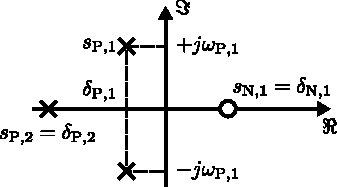
\includegraphics[width=0.48\linewidth]{Abbildungen/Modellbildung/PDF/PolNullstellen.pdf}
	\caption{Pol- Nullstellen Diagramm gebildet aus einer Übertragungsfunktion}
	\label{fig:polnullstellen}
\end{figure}
%
Wie in Abbildung~\ref{fig:polnullstellen} zu erkennen können Pole und Nullstellen sowohl reell als auch konjugiert komplex sein. Aus diesem Diagramm lassen sich jetzt direkt die zeitlichen Eigenschaften eines Systems ablesen.
%
\begin{itemize}
	\item \textbf{Dynamisches Verhalten}: 
		\begin{itemize}
			\item Sind die Pole reell ($s=\delta,\, j\omega = 0$)?
			\item Oder konjugiert komplex mit Dämpfung ($s=\delta\pm j\omega$)?
			\item Oder konjugiert komplex ohne Dämpfung ($s=\pm j\omega$)?
			\item Wie nahe sind sie der Imaginären Achse?
		\end{itemize}
		%
	\item \textbf{Stabilität}: 
		\begin{itemize}
			\item Sind alle Pole links der Imaginären Achse?
		\end{itemize}
\end{itemize}
%
\begin{Aufgaben}{}{}
	\begin{itemize}
		\item \textit{Einige Beispiele von Pol- Nullstellen Diagrammen und zugehörigen Zeitverläufen}
	\end{itemize}
\end{Aufgaben}
%
%###########################################################################
\subsubsection{Berechnung der Sprungantwort aus der Übertragungsfunktion}
%############################################################################
%
Es stellt sich die Frage, wie die Sprungantwort eines Systems nun aus der Übertragungsfunktion berechnet werden kann und welche Vorteile dies bietet. Berechnen wir mittels Partialbruchzerlegung aus der Multiplikation von \eqref{eq:polnullstellenform} und einem sprungförmigen Eingangssignal $U(s)$ nun die einzelnen Pole, ergibt sich folgende Gleichung
%
\begin{equation}
\begin{aligned}
Y(s)=G(s)U(s)=\frac{k_{0}}{s}+\frac{k_{1}}{\left(s-s_{\text{P},1}\right)}+\frac{k_{2}}{\left(s-s_{\text{P},2}\right)}+\ldots+\frac{k_{n}}{\left(s-s_{\text{P},n}\right)},\, k_{0}=\frac{b_{q}}{c_{p}}\label{eq:partialbrueche}\\
\end{aligned}
\end{equation}
%
Diese einzelnen Terme lassen sich mittels Laplace Rücktransformation nun in den Zeitbereich zurück übersetzen. Da wir in dieser Vorlesung lediglich LZI-Systeme betrachten, können die Einzelterme sowohl im Bild- als auch im Zeitbereich linear überlagert werden. Die Sprungantwort im Zeitbereich aus \eqref{eq:partialbrueche} ergibt sich zu 
%
\begin{equation}
\begin{aligned}
y(t)=h(t)=g(t)*u(t)=k_{0}+k_{1}e^{s_{\text{P},1}t}+k_{2}e^{s_{\text{P},2}t}+\ldots+k_{n}e^{s_{\text{P},n}t}\label{eq:sprungantwortlaplace}\\
\end{aligned}
\end{equation}
%
Diese Formulierung gilt nur für reellwertige Pole. Tauchen konjugiert komplexe Pole auf und sollen diese reellwertig dargestellt werden, so muss die Darstellung \eqref{eq:sprungantwortlaplace} erweitert werden, zu
%
\begin{equation*}
\begin{aligned}
%
Y(s)=G(s)U(s)=\frac{k_{1}}{\left(s-s_{\text{P},1}\right)}+\frac{k_{2}}{\left(s-s_{\text{P},2}\right)}\\
\text{mit}\,\, s_{\text{P},12}=\delta_{12}\pm j\omega_{12},\,\,k_{12}=\alpha_{12}\pm j\beta_{12}
%
\end{aligned}
\end{equation*}
%
Ausmultiplizieren und mittels eines Ansatzes lösen
%
\begin{equation*}
\begin{aligned}
%
Y(s)=G(s)U(s)=\frac{k_{1}\left(s-s_{\text{P},1}\right)+k_{2}\left(s-s_{\text{P},1}\right)}{\left(s-s_{\text{P},1}\right)\left(s-s_{\text{P},2}\right)}=\ldots=\frac{B_{1}s+B_{0}}{s^{2}+A_{1}s+A_{0}}
%
\end{aligned}
\end{equation*}
%
Durch Koeffizientenvergleich erhält man nun die reellen Koeffizienten 
%
\begin{equation*}
\begin{aligned}
%
B_{0}&=-2\left(\delta_{12}\alpha_{12}+\omega_{12}\beta_{12}\right)\\
B_{1}&=2\alpha_{12}\\
A_{0}&=\delta^{2}_{12}+\omega^{2}_{12}\\
A_{1}&=-2\delta_{12}
%
\end{aligned}
\end{equation*}
%
Diese Darstellung ist für die Rücktransformation günstiger da sie nur reelle Koeffizienten enthält und direkt über die Korrespondenztabelle abgelesen werden kann.
%
\newpage
%
%##################################################
\subsection{Lineare Grundglieder zur Beschreibung dynamischer Verhalten}
%##################################################
%
Im folgenden werden die wichtigsten linearen Grundglieder, welche für die Regelungstechnik Bedeutung haben vorgestellt. Die Inhalte dieses Kapitels können in \cite{Foellinger94, Unbehauen08, MSF05, Lunze10} nachgelesen werden.
%
%%##################################################
%\subsubsection{Proportionalglied (P-Glied)}
%%##################################################
%%
%Das Proportionalglied kennzeichnet sich durch einen konstanten Verstärkungsfaktor $K_{\text{p}}$ aus. Dieser ist aufgrund der Eigenschaften der Laplace Transformation im Zeit und im Bildbereich identisch.
%%
%\begin{itemize}
%%
%\item Funktionalbeziehung im Zeitbreich
%%
%\begin{equation*}
%\begin{aligned}
%%
%y(t)=K_{\text{p}}u(t)
%%
%\end{aligned}
%\end{equation*}
%%
%\item Laplacetransformierte und Übergangsfunktion im Bildbereich
%%
%\begin{equation*}
%\begin{aligned}
%%
%Y(s)=K_{\text{p}}U(s),\quad G(s)=K_{\text{p}},\quad H(s)=\frac{K_{\text{p}}}{s}
%%
%\end{aligned}
%\end{equation*}
%%
%\item Sprungantwort im Zeitbereich
%%
%\begin{figure}[h]
%	\centering
%	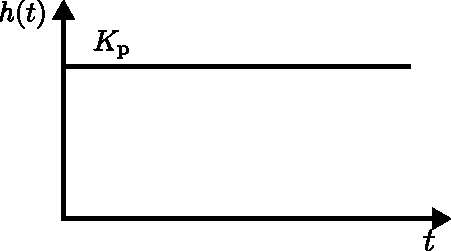
\includegraphics[width=0.375\linewidth]{Abbildungen/Modellbildung/PDF/PgliedSprung.pdf}
%	\caption{Qualitative Sprungantwort des Proportionalgliedes}
%	\label{fig:pgliedsprung}
%\end{figure}
%%
%\item Frequenzgang
%%
%\begin{equation*}
%\begin{aligned}
%%
%G(j\omega)=K_{\text{p}}
%%
%\end{aligned}
%\end{equation*}
%%
%\item Bodediagramm: Wird beim P-Glied vernachlässigt, da einfach.
%%
%\item Symbol bzw. Blockschaltbild
%%
%\begin{figure}[h]
%	\centering
%	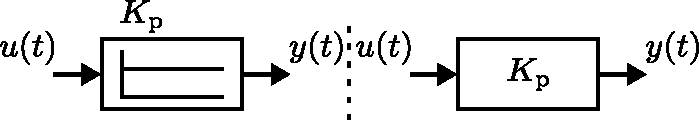
\includegraphics[width=0.65\linewidth]{Abbildungen/Modellbildung/PDF/PgliedBlock.pdf}
%	\caption{Symbol, Blockschaltbild des Proportionalgliedes}
%	\label{fig:pglied}
%\end{figure}
%%
%\end{itemize}
%%
%##################################################
\subsubsection{Integratorglied (I-Glied)}
%##################################################
%
Das I-Glied integriert den Eingang fortlaufend auf. $K_{\text{I}}=\frac{1}{T_{\text{I}}}$ stellt den Integrationsbeiwert dar. Dieser ist aufgrund der Eigenschaften der Laplace Transformation im Zeit und im Bildbereich identisch.
%
\begin{itemize}
	%
	\item Funktionalbeziehung und Darstellung im Zeitbreich
	%
	\begin{equation*}
	\begin{aligned}
	%
	y(t)=K_{\text{I}}\int_{0}^{t}u(\tau)\text{d}\tau \,\,\text{oder}\,\, y(t)=\frac{1}{T_{\text{I}}}\int_{0}^{t}u(\tau)\text{d}\tau
	%
	\end{aligned}
	\end{equation*}
	%
	\item Laplacetransformierte und Übergangsfunktion im Bildbereich
	%
	\begin{equation*}
	\begin{aligned}
	%
	Y(s)=\frac{K_{\text{I}}U(s)}{s},\quad G(s)=\frac{K_{\text{I}}}{s},\quad H(s)=\frac{K_{\text{I}}}{s^{2}}
	%
	\end{aligned}
	\end{equation*}
	%
	\item Pol- Nullstellen Diagramm im Bildbereich in Abbildung~\ref{fig:igliedpn}: Eine Polstelle im Ursprung vorhanden, zwar keinen negativen Realteil, aber definitionsgemäß instabil. 
	%
	\begin{figure}[h]
		\centering
		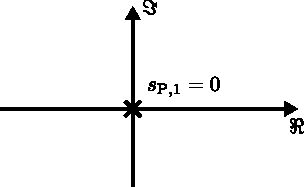
\includegraphics[width=0.4\linewidth]{Abbildungen/Modellbildung/PDF/Igliedpn.pdf}
		\caption{Qualitatives Pol- Nullstellen Diagramm des Integratorgliedes}
		\label{fig:igliedpn}
	\end{figure}
	%
	\item Sprungantwort im Zeitbereich: Ergibt sich aus der Rücktransformation von \\$H(s) \,\Laplace\, h(t)=K_{\text{I}}t$
	%
	\begin{figure}[h]
		\centering
		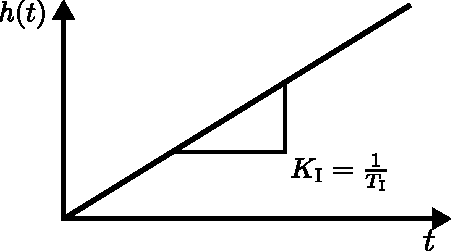
\includegraphics[width=0.375\linewidth]{Abbildungen/Modellbildung/PDF/IgliedSprung.pdf}
		\caption{Qualitative Sprungantwort des Integratorgliedes}
		\label{fig:igliedsprung}
	\end{figure}
	%
	\item Frequenzgang, Amplitudengang, Phasengang
	%
	\begin{equation*}
	\begin{aligned}
	%
	G(j\omega)&=\frac{K_{\text{I}}}{j\omega}= -j\frac{K_{\text{I}}}{\omega}\\
	%
	|G(j\omega)|_{\text{dB}}&=20\lg|G(j\omega)|=20\lg\left(\frac{K_{\text{I}}}{\omega}\right)\\
	%
	&=20\lg\left(K_{\text{I}}\right)-20\lg\left(\omega\right)\\
	%
	\angle G(j\omega)&=\arctan\left(\frac{-\frac{K_{\text{I}}}{\omega}}{0}\right)=-90^{\circ}\\
	\end{aligned}
	\end{equation*}
	%
	\item Bodediagramm in Abbildung~\ref{fig:igliedbode}: Die Durchtrittskreisfrequenz $\omega_{\text{D}}$ markiert den Punkt bei der die Verstärkung gleich $1$ oder $0$ dB ist. Der Amplitudengang kennzeichnet sich durch eine negative Steigung von $\frac{-20\text{dB}}{Dek.}$. Da der Phasengang sich nur aus negativen komplexen Anteilen zusammensetzt ist die Phase von Anfang an $-90^{\circ}$.\\\\
	%
	\begin{figure}[h]
		\centering
		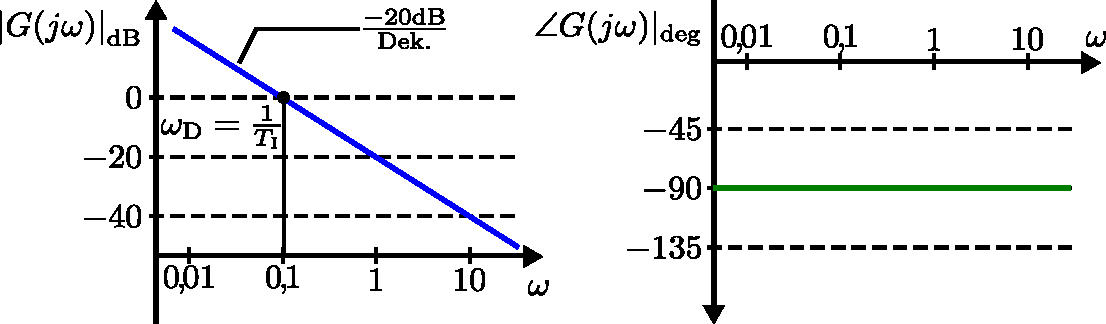
\includegraphics[width=0.85\linewidth]{Abbildungen/Modellbildung/PDF/IgliedBode.pdf}
		\caption{Qualitatives Bodediagramm des Integratorglieds}
		\label{fig:igliedbode}
	\end{figure}
	%
	\item Symbol bzw. Blockschaltbild in Abbildung~\ref{fig:igliedblock}
	%
	\begin{figure}[h]
		\centering
		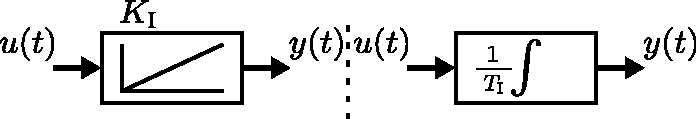
\includegraphics[width=0.625\linewidth]{Abbildungen/Modellbildung/PDF/IgliedBlock.pdf}
		\caption{Symbol, Blockschaltbild des Integratorglieds}
		\label{fig:igliedblock}
	\end{figure}
%
\end{itemize}
%
%##################################################
\subsubsection{Differenzierglied (D-Glied)}
%##################################################
%
Das Differenzierglied leitet den Eingang $u(t)$ kontinuierlich ab. Zudem exitiert ein Verstärkungsfaktor $K_{\text{D}}$. Dieser ist aufgrund der Eigenschaften der Laplace Transformation im Zeit und im Bildbereich identisch.
%
\begin{itemize}
	%
	\item Funktionalbeziehung und Darstellung im Zeitbreich
	%
	\begin{equation*}
	\begin{aligned}
	%
	y(t)=K_{\text{D}}\frac{\text{d}u(t)}{\text{d}t}
	%
	\end{aligned}
	\end{equation*}
	%
	\item Laplacetransformierte und Übergangsfunktion im Bildbereich
	%
	\begin{equation*}
	\begin{aligned}
	%
 	Y(s)=K_{\text{D}}U(s)s,\quad G(s)=K_{\text{D}}s,\quad H(s)=K_{\text{D}}
	%
	\end{aligned}
	\end{equation*}
	%
	\item Pol- Nullstellen Diagramm im Bildbereich in Abbildung~\ref{fig:dgliedpn}: Differenzierglied besitzt eine Nullstelle im Ursprung. Das System ist je nach Definition stabil; Zustandsstabil da kein Pol in der rechten Halbebene, jedoch nicht E/A-stabil, da auch Sprungstellen des Eingangssignals abgeleitet werden. Somit können unbegrenzte Ableitungen auftreten (theoretisch).
	%
	\begin{figure}[h]
		\centering
		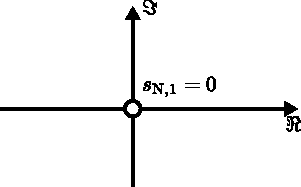
\includegraphics[width=0.4\linewidth]{Abbildungen/Modellbildung/PDF/Dgliedpn.pdf}
		\caption{Qualitatives Pol- Nullstellen Diagramm des Diffenzierglieds}
		\label{fig:dgliedpn}
	\end{figure}
	%
	%
	\item Sprungantwort im Zeitbereich: Ergibt sich aus der Rücktransformation von \\$H(s) \,\Laplace\, h(t)=K_{\text{D}}\delta(t)$. Eigenschaft des Dirac-Impuls
	%
	\begin{equation*}
	\begin{aligned}
	%
	\int_{-\infty}^{\infty}h(\tau)\text{d}\tau=K_{\text{D}}
	%
	\end{aligned}
	\end{equation*}
	%
	Ist ein Rechteck mit der Fläche $K_{\text{D}}$, welches infinitisimal schmal ist.
	%
	\item Frequenzgang, Amplitudengang, Phasengang
	%
	\begin{equation*}
	\begin{aligned}
	%
	G(j\omega)&=K_{\text{D}}j\omega\\
	%
	|G(j\omega)|_{\text{dB}}&=20\lg|G(j\omega)|=20\lg\left(K_{\text{D}}\omega\right)=20\lg\left(K_{\text{D}}\right)+20\lg\left(\omega\right)\\
	%
	\angle G(j\omega)&=\arctan\left(\frac{K_{\text{D}}\omega}{0}\right)=+90^{\circ}\\
	\end{aligned}
	\end{equation*}
	%
	\item Bodediagramm: Die Durchtrittskreisfrequenz $\omega_{\text{D}}$ markiert den Punkt bei der die Verstärkung gleich $1$ oder $0$ dB ist. Der Amplitudengang kennzeichnet sich durch eine positive Steigung von $\frac{+20\text{dB}}{Dek.}$. Da der Phasengang sich nur aus positiven komplexen Anteilen zusammensetzt ist die Phase von Anfang an $+90^{\circ}$.
	%
	\begin{figure}[h]
		\centering
		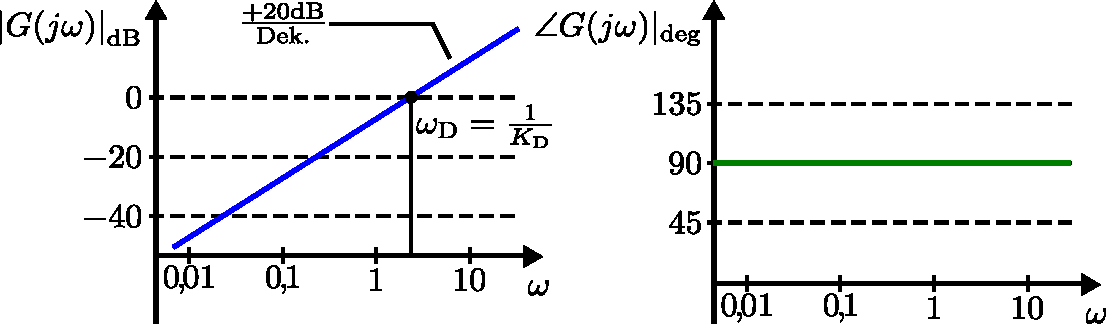
\includegraphics[width=0.8\linewidth]{Abbildungen/Modellbildung/PDF/DgliedBode.pdf}
		\caption{Qualitatives Bodediagramm des Differenzierglied}
		\label{fig:dgliedbode}
	\end{figure}
	%
	\item Symbol bzw. Blockschaltbild
	%
	\begin{figure}[h]
		\centering
		\includegraphics[width=0.65\linewidth]{Abbildungen/Modellbildung/PDF/DgliedBlock.pdf}
		\caption{Symbol, Blockschaltbild des Differenzierglied}
		\label{fig:dglied}
	\end{figure}
	%
\end{itemize}
%
%##################################################
\subsubsection{Totzeitglied (T$_{\boldsymbol{t}}$-Glied)}
%##################################################
%
Das Totzeitglied, zeichnet sich durch eine durch eine Verschiebungsfunktion aus, welche eine beliebige Zeitfunktion um einen konstanten Wert $T_{t}$ nach rechts verschiebt.
%
\begin{itemize}
	%
	\item Funktionalbeziehung
	%
	\begin{equation*}
	\begin{aligned}
	%
	y(t)=u(t-T_{t})
	%
	\end{aligned}
	\end{equation*}
	%
	\item Laplacetransformierte und Übergangsfunktion im Bildbereich
	%
	\begin{equation*}
	\begin{aligned}
	%
	Y(s)=e^{-T_{t}s}U(s),\quad G(s)=e^{-T_{t}s},\quad H(s)=\frac{e^{-T_{t}s}}{s}
	%
	\end{aligned}
	\end{equation*}
	%
	\item Pol- Nullstellen Diagramm im Bildbereich: Das Totzeitglied hat kein eigenes Diagramm, da es keine Pole oder Nullstellen besitzt.
	%
	\item Sprungantwort im Zeitbereich in Abbildung~\ref{fig:tgliedsprung}: Ergibt sich aus der Rücktransformation von \\$H(s) \,\Laplace\, h(t)=\sigma(t-T_{t})$.
	%
	\begin{figure}[h]
		\centering
		\includegraphics[width=0.4\linewidth]{Abbildungen/Modellbildung/PDF/TgliedSprung.pdf}
		\caption{Qualitative Sprungantwort des Totzeitgliedes}
		\label{fig:tgliedsprung}
	\end{figure}
	%
	\item Frequenzgang, Amplitudengang, Phasengang
	%
	\begin{equation*}
	\begin{aligned}
	%
	G(j\omega)&=e^{-T_{t}j\omega}=\cos(\omega T_{t})-j\sin(\omega T_{t})\\
	%
	|G(j\omega)|_{\text{dB}}&=20\lg|G(j\omega)|=20\lg\left(\underbrace{\sqrt{\cos^{2}(\omega T_{t})+\sin^{2}(\omega T_{t})}}_{=1}\right)=0\\
	%
	\angle G(j\omega)&=\arctan\left(\frac{-\sin(\omega T_{t})}{\cos(\omega T_{t})}\right)=-\omega T_{t}\\
	\end{aligned}
	\end{equation*}
	%
	\item Bodediagramm in Abbildung~\ref{fig:tgliedbode}: Der Amplitudengang des Totzeitgliedes ist eine konstante Linie mit der Verstärkung 1 in dB. Der Phasengang auf der anderen Seite ergibt sich als eine stark abfallende Funktion der Kreisfrequenz $\omega$. Der Phasengang hat bei $\omega=\frac{1}{T_{t}}$ eine Phase von $-57^{\circ}$.
	%
	\begin{figure}[h]
		\centering
		\includegraphics[width=0.9\linewidth]{Abbildungen/Modellbildung/PDF/TgliedBode.pdf}
		\caption{Qualitatives Bodediagramm des Totzeitgliedes}
		\label{fig:tgliedbode}
	\end{figure}
	%
	\item Symbol bzw. Blockschaltbild
	%
	\begin{figure}[h]
		\centering
		\includegraphics[width=0.3\linewidth]{Abbildungen/Modellbildung/PDF/TgliedBlock.pdf}
		\caption{Symbol, Blockschaltbild des Totzeitgliedes}
		\label{fig:tglied}
	\end{figure}
	%
\end{itemize}
%
%##################################################
\subsubsection{Verzögerungsglied 1-Ordnung (PT$_{\boldsymbol{1}}$-Glied)}
%##################################################
%
Das Verzögerungsglied erster Ordnung beschreibt ein dynamisches Verhalten wie es bei einer Differentialgleichung erster Ordnung vorkommt. Die Beiden beschreibenden Variablen ist die Zeitkonstante $T_{1}$ und der Verstärkungsfaktor $K_{\text{p}}$.
%
\begin{itemize}
	%
	\item Funktionalbeziehung im Zeitbereich
	%
	\begin{equation*}
	\begin{aligned}
	%
	T_{1}\frac{\text{d}y(t)}{\text{d}}+y(t)=K_{\text{p}}u(t)
	%
	\end{aligned}
	\end{equation*}
	%
	\item Laplacetransformierte, Übertragungsfunktion und Übergangsfunktion im Bildbereich
	%
	\begin{equation*}
	\begin{aligned}
	%
	Y(s)=\frac{K_{\text{p}}}{T_{1}s+1}U(s),\quad G(s)=\frac{K_{\text{p}}}{T_{1}s+1},\quad H(s)=\frac{K_{\text{p}}}{s\left(T_{1}s+1\right)}
	%
	\end{aligned}
	\end{equation*}
	%
	\item Pol- Nullstellen Diagramm im Bildbereich in Abbildung~\ref{fig:pt1gliedpn}: Das $\text{PT}_{1}-\text{Glied}$ besitzt eine Polstellen in der negativen Halbebene bei $s_{\text{P},1}=-\frac{1}{T_{1}}$ und keine Nullstelle. Da technische Systeme immer eine Positive (physikalische) Zeitkonstante besitzen ist diese Glied zunächst einmal stabil.
	%
	\begin{figure}[h]
		\centering
		\includegraphics[width=0.4\linewidth]{Abbildungen/Modellbildung/PDF/PT1gliedpn.pdf}
		\caption{Qualitatives Pol- Nullstellen Diagramm des Verzögerungsgliedes 1-Ordnung}
		\label{fig:pt1gliedpn}
	\end{figure}
	%
	%
	\item Sprungantwort im Zeitbereich in Abbildung~\ref{fig:pt1gliedsprung}: Ergibt sich aus der Rücktransformation von $H(s) \,\Laplace\, h(t)=K_{\text{p}}\left(1-e^{-\frac{t}{T_{1}}}\right)$. Sowohl $K_{\text{p}}$ als auch $T_{1}$ lassen sich aus der Sprungantwort ermitteln.
	%
	\begin{figure}[h]
		\centering
		\includegraphics[width=0.4\linewidth]{Abbildungen/Modellbildung/PDF/PT1gliedSprung.pdf}
		\caption{Qualitative Sprungantwort des Verzögerungsglied 1-Ordnung}
		\label{fig:pt1gliedsprung}
	\end{figure}
	%
	\item Frequenzgang, Amplitudengang, Phasengang
	%
	\begin{equation*}
	\begin{aligned}
	%
		G(j\omega)&=\frac{K_{\text{P}}}{T_{1}j\omega+1}=\frac{K_{\text{P}}}{T_{1}j\omega+1}\cdot\frac{-T_{1}j\omega+1}{-T_{1}j\omega+1}=\frac{K_{\text{P}}\left(1-T_{1}j\omega\right)}{T^{2}_{1}\omega^{2}+1}\\
	%
	|G(j\omega)|_{\text{dB}}&=20\lg|G(j\omega)|=20\lg\left(\frac{K_{\text{p}}}{\sqrt{T^{2}_{1}\omega^{2}+1}}\right)\\
	%
	&=20\lg\left(K_{\text{p}}\right)-20\lg\left(\sqrt{T_{1}^{2}\omega^{2}+1}\right)\\
	%
	\angle G(j\omega)&=\arctan\left(\frac{-\frac{K_{\text{p}}\omega T_{1}}{T^{2}_{1}\omega^{2}+1}}{\frac{K_{\text{p}}}{T^{2}_{1}\omega^{2}+1}}\right)=\arctan\left(-\omega T_{1}\right)=-\arctan\left(\omega T_{1}\right)\\
	\end{aligned}
	\end{equation*}
	%
	\item Bodediagramm in Abbildung~\ref{fig:pt1gliedbode}: Bis zum erreichen der Knickfrequenz $\omega_{\text{E}}$ verläuft der Amplitudengang Frequenz unabhängig mit der Verstärkung $K_{\text{p}}$ in dB. Durch die Vergrößerung der Frequenz $\omega$ wird nun auch der zweite (frequenzabhängige) Term des Amplitudengangs relevant und er neigt sich bis zu einer negativen Steigung von $\frac{-20\text{dB}}{\text{Dek.}}$. Der Phasengang verhält sich zunächst auch konstant und nimmt den Wert $0^{\circ}$ an. Er fällt auf einen Wert von $-90^{\circ}$ für $\omega\rightarrow\infty$. In Höhe der Knickfrequenz $\omega_{\text{E}}$ ist die Phase $-45^{\circ}$.
	%
	\begin{figure}[h]
		\centering
		\includegraphics[width=0.9\linewidth]{Abbildungen/Modellbildung/PDF/PT1gliedBode.pdf}
		\caption{Qualitatives Bodediagramm des Verzögerungsglied 1-Ordnung}
		\label{fig:pt1gliedbode}
	\end{figure}
	%
	\item Symbol bzw. Blockschaltbild
	%
	\begin{figure}[h]
		\centering
		\includegraphics[width=0.3\linewidth]{Abbildungen/Modellbildung/PDF/PT1gliedBlock.pdf}
		\caption{Symbol, Blockschaltbild des Verzögerungsglied 1-Ordnung}
		\label{fig:pt1glied}
	\end{figure}
	%
\end{itemize}
%
%##################################################
\subsubsection{Verzögerungsglied 2ter-Ordnung (PT$_{\boldsymbol{2}}$-Glied)}
%##################################################
%
Das Verzögerungsglied zweiter Ordnung kann genutzt werden, um dynamische Systeme darzustellen, welche durch eine lineare Differentialgleichung 2ter-Ordnung ausgedrückt werden können (z.B. elektrischer Schwingkreis oder Kette von RC-Gliedern).
%
\begin{itemize}
	%
	\item Funktionalbeziehung im Zeitbereich
	%
	\begin{equation*}
	\begin{aligned}
	%
	T^{2}\frac{\text{d}^{2}y(t)}{\text{d}t^{2}}+2dT\frac{\text{d}y(t)}{\text{d}t}+y(t)=K_{\text{p}}u(t)
	%
	\end{aligned}
	\end{equation*}
	%
	Laplacetransformierte und Übergangsfunktion im Bildbereich
	%
	\begin{equation*}
	\begin{aligned}
	%
	Y(s)=\frac{K_{\text{p}}}{T^{2}s^{2}+2dTs+1}U(s),\quad G(s)=\frac{K_{\text{p}}}{T^{2}s^{2}+2dTs+1}\\ H(s)=\frac{K_{\text{p}}}{s\left(T^{2}s^{2}+2dTs+1\right)}
	%
	\end{aligned}
	\end{equation*}
	%
	Die Übertragungsfunktion lässt sich durch Umformung folgendermaßen darstellen
	%
	\begin{equation*}
	\begin{aligned}
	%
	G(s)&=\frac{K_{\text{p}}}{T^{2}s^{2}+2dTs+1}\\
	%
	&=\frac{K_{\text{p}}}{\frac{1}{\omega^{2}_{0}}s^{2}+\frac{2d}{\omega_{0}}s+1}, \quad \omega_{0} = \frac{1}{T}\\
	%
	&=\frac{K_{\text{p}}\omega^{2}_{0}}{s^{2}+2d\omega_{0}s+\omega^{2}_{0}}
	%
	\end{aligned}
	\end{equation*}
	%
	Und die Pole nach folgender Vorschrift berechnen
	%
	\begin{equation*}
	\begin{aligned}
	%
	&s^{2}+2d\omega_{0}s+\omega^{2}_{0}=0\\
	%
	&s_{\text{P},12}=-d\omega_{0}\pm\sqrt{d^{2}\omega^{2}_{0}-\omega^{2}_{0}}\\
	%
	&s_{\text{P},12}=-d\omega_{0}\pm\omega_{0}\sqrt{d^{2}-1}\\
	%
	\end{aligned}
	\end{equation*}
	%
	\item Pol- Nullstellen Diagramm im Bildbereich in Abbildung~\ref{fig:pt2gliedpn}: Das $\text{PT}_{2}-\text{Glied}$ hat, je nachdem welche Dämpfung $d$ das System besitzt, unterschiedliche Pole und keine Nullstelle. In Abbildung~\ref{fig:pt2gliedpn} sind die beiden Fälle für $d<1$ (konjugiert komplexe Polpaar) und $d=1$ (doppelter Reeller Pol) dargestellt. Für $d>1$ ergeben sich zwei unterschiedliche reele Polstellen. Für eine negative Dämpfung $d<0$ schwingt das system auf und wird instabil. Jenachdem welchen negativen Dämpfungwert das System hat ist es entweder aperiodisch oder schwingend.
	%
	\begin{figure}[h]
		\centering
		\includegraphics[width=0.6\linewidth]{Abbildungen/Modellbildung/PDF/PT2gliedpn.pdf}
		\caption{Qualitatives Pol- Nullstellen Diagramm des Verzögerungsgliedes 2ter-Ordnung für konjugiert komplexe und reelle Polpaare und deren Sprungantworten}
		\label{fig:pt2gliedpn}
	\end{figure}
	%
	%
	\item Sprungantwort im Zeitbereich: Hierfür muss zunächst eine Fallunterscheidung getroffen werden
	%
	\begin{equation*}
	\begin{aligned}
	%
	0<d<1 \rightarrow H(s)\,\laplace\,h(t)&=\\
	K_{\text{p}}\left[1-\frac{1}{\sqrt{d^{2}-1}}\right.&\left.\cdot e^{-d\omega_{0}t}\cdot\sin\left(\left(\omega_{0}\sqrt{d^{2}-1}\right)t+\text{arccos}(d)\right)\right]\\
	%
	d>1 \rightarrow H(s)\,\laplace\,h(t)&= K_{\text{p}}\left(1-\frac{T_{1}}{T_{1}-T_{2}}e^{-\frac{t}{T_{1}}}+\frac{T_{2}}{T_{1}-T_{2}}e^{-\frac{t}{T_{2}}}\right)\\
	%
	d=1 \rightarrow H(s)\,\laplace\,h(t)&= K_{\text{p}}\left(1-e^{-\frac{t}{T}}\left(1+\frac{t}{T}\right)\right)\\
	%
	d=0 \rightarrow H(s)\,\laplace\,h(t)&= K_{\text{p}}\left(1-\cos\left(\omega_{0}t\right)\right)
	%
	\end{aligned}
	\end{equation*}
	%
	\begin{figure}[h]
		\centering
		\includegraphics[width=0.9\linewidth]{Abbildungen/Modellbildung/PDF/PT2gliedSprung.pdf}
		\caption{Qualitative Sprungantworten des Verzögerungsglied 2ter-Ordnung}
		\label{fig:pt2gliedsprung}
	\end{figure}
	%
	\item Frequenzgang, Amplitudengang, Phasengang
	%
	\begin{equation*}
	\begin{aligned}
	%
	G(j\omega)&=\frac{K_{\text{p}}}{\frac{(j\omega)^{2}}{\omega_{0}^{2}}+2d\frac{j\omega}{\omega_{0}}+1}\\
	%
	&=\frac{K_{\text{p}}}{1-\frac{\omega^{2}}{\omega_{0}^{2}}+j2d\frac{\omega}{\omega_{0}}}=\frac{K_{\text{p}}\left[1-\frac{\omega^{2}}{\omega_{0}^{2}}\right]-jK_{\text{p}}\left[2d\frac{\omega}{\omega_{0}}\right]}{\left[1-\frac{\omega^{2}}{\omega_{0}^{2}}\right]^{2}+\left[2d\frac{\omega}{\omega_{0}}\right]^{2}}\\
	%
	|G(j\omega)|_{\text{dB}}&=20\lg|G(j\omega)|=20\lg\left(\frac{K_{\text{p}}}{\sqrt{\left[1-\frac{\omega^{2}}{\omega_{0}^{2}}\right]^{2}+\left[2d\frac{\omega}{\omega_{0}}\right]^{2}}}\right)\\
	%
	&=20\lg\left(K_{\text{p}}\right)-20\lg\left(\sqrt{\left[1-\frac{\omega^{2}}{\omega_{0}^{2}}\right]^{2}+\left[2d\frac{\omega}{\omega_{0}}\right]^{2}}\right)\\
	%
	\angle G(j\omega)&=\arctan\left(\frac{-\left[2d\frac{\omega}{\omega_{0}}\right]}{\left[1-\frac{\omega^{2}}{\omega_{0}^{2}}\right]}\right)=-\arctan\left(\frac{\left[2d\frac{\omega}{\omega_{0}}\right]}{\left[1-\frac{\omega^{2}}{\omega_{0}^{2}}\right]}\right)
	%
	\end{aligned}
	\end{equation*}
	%
	\item Bodediagramm
	%
	\begin{figure}[h]
		\centering
		\includegraphics[width=0.9\linewidth]{Abbildungen/Modellbildung/PDF/PT2gliedBode.pdf}
		\caption{Qualitatives Bodediagramm des Verzögerungsglied 2-Ordnung}
		\label{fig:pt2gliedbode}
	\end{figure}
	%
	Anmerkungen zum Bodediagramm: Der Amplituden- und Phasengang ist je nach Dämpfung unterschiedlich:
	\begin{itemize}
		\item $0<d<1$ \textbf{Konjugiert komplexes Polpaar}: Das Verhalten im Bodediagramm ist vergleichbar mit der Resonanz beim Reihenschwingkreis, die Amplitude wird durch den elektrischen Widerstand in der Schaltung begrenzt. Hier ist die Dämpfung $d$ der entscheidende Faktor. Der asymptotische Amplitudengang knickt bei $\omega_{\text{E}}=\omega_{0}$ um $\frac{-40\text{dB}}{Dek.}$ ab. Der tatsächliche Amplitudengang ist in Abbildung~\ref{fig:pt2gliedbode} links unten dargestellt. Die Resonanzüberhöhung entsteht bei $\omega=\omega_{\text{e}}\neq\omega_{0}$. Der Phasengang ist ebenso vom Dämpfungsbeiwert abhängig, je kleiner der Wert, desto steiler verläuft der Phasengang. Der Phasengang startet bei $0^{\circ}$ und verläuft für $\omega\rightarrow \infty$ gegen $-180^{\circ}$
		% 
		\item $d=1$ \textbf{Doppelter reeller Pol}: Aperiodischer Grenzfall, der asymptotische Amplitudengang knickt bei $\omega=\omega_{0}$ um $\frac{-40\text{dB}}{\text{Dek.}}$ ab. Die Durchtrittskreisfrequenz $\omega_{\text{D}}$ wird durch den Verstärkungsbeiwert $K_{\text{p}}$ und durch die Knickfrequenz $\omega_{\text{E}}$ festgelegt. Die Knickfrequenz $\omega_{\text{E}}$ ist bei einer Dämpfung $d=1$ identisch mit $\omega_{0}$. Der Phasengang verläuft wie beim $\text{PT}_{1}-\text{Glied}$ jedoch mit einer Steigung von $\frac{-90^{\circ}}{\text{Dek.}}$. In Höhe der Knickfrequenz ist die Phase $-90^{\circ}$. Der Phasengang startet bei $0^{\circ}$ und verläuft für $\omega\rightarrow \infty$ gegen $-180^{\circ}$
		%
		\item $d>1$ \textbf{Zwei unterschiedliche reelle Pole}: In diesem Fall lässt sich der Amplitudengang wie bei zwei hintereinander geschalteten  $\text{PT}_{1}-\text{Gliedern}$ realisieren. Das Bedeutet das jedes  $\text{PT}_{1}-\text{Glied}$ einen Beitrag zum Amplitudengang ab der jeweiligen Knickfrequenz $\omega_{\text{E},1}$ von $\frac{-20\text{dB}}{\text{Dek.}}$ liefert. Die Steigungen der einzelnen Anteile addieren sich auf, sodass nach der zweiten Knickfrequenz $\omega_{\text{E},2}$ der Amplitudengang eine negative Steigung von $\frac{-40\text{dB}}{\text{Dek.}}$ aufweist. Gleiches gilt für den Phasengang, welcher sich analog zum $\text{PT}_{1}-\text{Glied}$ realisieren lässt. Es muss beachtet werden, dass sich die Wirkung der beiden Pole auf den Phasengang auch überlagern, was bei sehr nahe aneinander liegenden Polen zu einer Steigung der Phasengangs von bis zu $\frac{-90^{\circ}}{\text{Dek.}}$ führt. Der Phasengang startet bei $0^{\circ}$ und verläuft für $\omega\rightarrow \infty$ gegen $-180^{\circ}$
	\end{itemize}
	%
	\item Symbol bzw. Blockschaltbild
	%
	\begin{figure}[h]
		\centering
		\includegraphics[width=0.3\linewidth]{Abbildungen/Modellbildung/PDF/PT2gliedBlock.pdf}
		\caption{Symbol, Blockschaltbild des Verzögerungsglied 2-Ordnung}
		\label{fig:pt2glied}
	\end{figure}
	%
\end{itemize}
%
\begin{simulation}{}{}
	\begin{itemize}
		\item \textit{Verzögerungsglied 2-Ordnung}
	\end{itemize}
\end{simulation}
%
%%##################################################
%\subsubsection{Verzögerungsglied n-Ordnung (PT$_{\boldsymbol{n}}$-Glied)}
%%##################################################
%%
%Das Verzögerungslied $n$ter-Ordnung, welches eine Verallgemeinerung des PT$_{\boldsymbol{1}}$-Glieds darstellt, lässt sich durch die Aneinanderreihung mehrerer Verzögerungslieder 1ter-Ordnung beschreiben. Mit ihm lassen sich lineare Differentialgleichungen höherer Ordnung abbilden, welche in technischen Prozessen regelmäßig vorkommen.
%%
%\begin{itemize}
%	%
%	\item Funktionalbeziehung im Zeitbereich
%	%
%	\begin{equation*}
%	\begin{aligned}
%	T_{n}\frac{\text{d}^{n}y(t)}{\text{d}t^{n}}+&T_{n-1}\frac{\text{d}^{n-1}y(t)}{\text{d}t^{n-1}}+\cdots+T_{1}\frac{\text{d}y(t)}{\text{d}t}+y(t)=K_{\text{p}}u(t)\\
%	\end{aligned}
%	\end{equation*}
%	%
%	\item Laplacetransformierte und Übergangsfunktion im Bildbereich
%	%
%	\begin{equation*}
%	\begin{aligned}
%	%
%	Y(s)=\frac{K_{\text{p}}}{\left(Ts+1\right)^{n}}U(s),\quad G(s)=\frac{K_{\text{p}}}{\left(Ts+1\right)^{n}},\quad H(s)=\frac{K_{\text{p}}}{s\left(Ts+1\right)^{n}}
%	%
%	\end{aligned}
%	\end{equation*}
%	%
%	\item Sprungantwort im Zeitbereich in Abbildung~\ref{fig:ptngliedsprung}: Für den Spezialfall $n=2$ aus vorheriger Berechnung $d=1$ $H(s)\,\laplace\,h(t)= K_{\text{p}}\left(1-e^{-\frac{t}{T}}\left(1+\frac{t}{T}\right)\right)$
%	%
%	\begin{figure}[h]
%		\centering
%		\includegraphics[width=0.4\linewidth]{Abbildungen/Modellbildung/PDF/PTngliedSprung.pdf}
%		\caption{Qualitative Sprungantwort des Verzögerungsglied n-Ordnung}
%		\label{fig:ptngliedsprung}
%	\end{figure}
%	%
%	\item Frequenzgang: Wird hier übersprungen, für den Spezialfall $n=2$ kann er aus dem vorherigen Beispiel des PT$_{\boldsymbol{2}}$-Gliedes berechnet werden. 
%	%
%	\item Bodediagramm: Ergibt sich aus der additiven Überlagerung der einzelnen PT$_{\boldsymbol{1}}$-Gliedern.
%	%
%	\item Symbol bzw. Blockschaltbild
%	%
%	\begin{figure}[h]
%		\centering
%		\includegraphics[width=0.7\linewidth]{Abbildungen/Modellbildung/PDF/PTngliedBlock.pdf}
%		\caption{Symbol, Blockschaltbild des Verzögerungsgliedes n-Ordnung}
%		\label{fig:ptnglied}
%	\end{figure}
%	%
%\end{itemize}
%%
%%############################################################################
%\subsubsection{Differenzierglied 1-Ordnung (DT$_{\boldsymbol{1}}$-Glied)}
%%###########################################################################
%%
%Das reale Differenzierglied wird aus der Reihenschaltung eines Differenzierglieds und eines PT$_{\boldsymbol{1}}$-Glieds gebildet.
%%
%\begin{itemize}
%	%
%	\item Funktionalbeziehung im Zeitbereich
%	%
%	\begin{equation*}
%	\begin{aligned}
%	%
%	T_{1}\frac{\text{d}y(t)}{\text{d}t}+y(t)=K_{\text{D}}\frac{\text{d}u(t)}{\text{d}t}
%	%
%	\end{aligned}
%	\end{equation*}
%	%
%	\item Laplacetransformierte und Übergangsfunktion im Bildbereich
%	%
%	\begin{equation*}
%	\begin{aligned}
%	%
%	Y(s)=\frac{K_{\text{D}}s}{\left(T_{1}s+1\right)}U(s),\quad G(s)=\frac{K_{\text{D}}s}{\left(T_{1}s+1\right)},\quad H(s)=\frac{K_{\text{D}}}{\left(T_{1}s+1\right)}
%	%
%	\end{aligned}
%	\end{equation*}
%	%
%	\item Pol- Nullstellen Diagramm im Bildbereich in Abbildung~\ref{fig:dt1gliedpn}: Das $\text{DT}_{1}-\text{Glied}$ besitzt eine Nullstelle im Ursprung $s_{\text{N},1}=0$ und einen Pol bei $s_{\text{P},1}=-\frac{1}{T_{1}}$
%	%
%	\begin{figure}[h]
%		\centering
%		\includegraphics[width=0.4\linewidth]{Abbildungen/Modellbildung/PDF/DT1gliedpn.pdf}
%		\caption{Qualitatives Pol- Nullstellen Diagramm des Differenziergliedes 1ter-Ordnung}
%		\label{fig:dt1gliedpn}
%	\end{figure}
%	%
%	%
%	\item Sprungantwort im Zeitbereich in Abbildung~\ref{fig:dt1gliedsprung}: Laplace Rücktransformation von $H(s)\,\laplace\,h(t)= \frac{K_{\text{p}}}{T_{1}}e^{-\frac{t}{T_{1}}}$
%	%
%	\begin{figure}[h]
%		\centering
%		\includegraphics[width=0.4\linewidth]{Abbildungen/Modellbildung/PDF/DT1gliedSprung.pdf}
%		\caption{Qualitative Sprungantwort des Differenzierglied 1-Ordnung}
%		\label{fig:dt1gliedsprung}
%	\end{figure}
%	%
%	\item Frequenzgang, Amplitudengang, Phasengang
%	%
%	\begin{equation*}
%	\begin{aligned}
%	%
%	G(j\omega)&=\frac{K_{\text{D}}j\omega}{T_{1}j\omega+1}=\frac{K_{\text{D}}j\omega}{T_{1}\omega+1}\cdot\frac{-T_{1}j\omega+1}{-T_{1}j\omega+1}=\frac{K_{\text{D}}\left(j\omega+T_{1}\omega^{2}\right)}{T^{2}_{1}\omega^{2}+1}\\
%	%
%	|G(j\omega)|_{\text{dB}}&=20\lg|G(j\omega)|=20\lg\left(\frac{K_{\text{D}}\omega}{\sqrt{T^{2}_{1}\omega^{2}+1}}\right)\\
%	%
%	&=20\lg\left(K_{\text{D}}\omega\right)-20\lg\left(\sqrt{T_{1}^{2}\omega^{2}+1}\right)\\
%	%
%	\angle G(j\omega)&=\arctan\left(\frac{\frac{K_{\text{D}}\omega}{T^{2}_{1}\omega^{2}+1}}{\frac{K_{\text{D}}T_{1}\omega^{2}}{T^{2}_{1}\omega^{2}+1}}\right)=\arctan\left(\frac{\omega}{T_{1}\omega^{2}}\right)=\arctan\left(\frac{1}{\omega T_{1}}\right)\\
%	\end{aligned}
%	\end{equation*}
%	%
%	\item Bodediagramm in Abbildung~\ref{fig:dt1gliedbode}: Der Amplitudengang startet bei $-\infty$ und besitzt eine positive Steigung von $\frac{+20\text{dB}}{\text{Dek.}}$ identisch zum D-Glied. Die Durchtrittskreisfrequenz $\omega_{\text{D}}$ ergibt sich aus der Verstärkung  $K_{\text{D}}$. Durch den Anteil des $\text{PT}_{1}-\text{Gliedes}$ knickt der Amplitudengang an der Eckfrequenz $\omega_{E}$, da hier ein Beitrag von $\frac{-20\text{dB}}{\text{Dek.}}$ von hinzukommt. In Summe wird der Amplitudengang ab dieser Frequenz invariant gegenüber weiteren Frequenzerhöhungen. Der Phasengang beginnt bei $+90^{\circ}$, identisch wie im Falle des D-Gliedes und fällt durch den Anteil des  $\text{PT}_{1}-\text{Gliedes}$ auf $0^{\circ}$ für $\omega\rightarrow\infty$. An der Eckfrequenz $\omega_{E}$ beträgt die Phase $+45^{\circ}$.
%	%
%	\begin{figure}[ht]
%		\centering
%		\includegraphics[width=0.9\linewidth]{Abbildungen/Modellbildung/PDF/DT1gliedBode.pdf}
%		\caption{Qualitatives Bodediagramm des Differenzierglied 1-Ordnung}
%		\label{fig:dt1gliedbode}
%	\end{figure}
%	%
%	\item Symbol bzw. Blockschaltbild
%	%
%	\begin{figure}[ht]
%		\centering
%		\includegraphics[width=0.45\linewidth]{Abbildungen/Modellbildung/PDF/DT1gliedBlock.pdf}
%		\caption{Symbol, Blockschaltbild des Differenzierglied 1-Ordnung}
%		\label{fig:dt1glied}
%	\end{figure}
%	%
%\end{itemize}
%
%######################################################################
% Erläuzterung zu den Rechenregeln einfügen
%######################################################################
%
\begin{Summary}{}{}
	\begin{itemize}
		\item \textit{Berechnen und zeichnen Sie $\angle G(j\omega)$ und $|G(j\omega)|_{\text{dB}}$ eines IT$_{\boldsymbol{1}}$-Gliedes.}
		\item \textit{Berechnen und zeichnen Sie $\angle G(j\omega)$ und $|G(j\omega)|_{\text{dB}}$ eines PT$_{\boldsymbol{3}}$-Gliedes.}
		\item \textit{Berechnen und zeichnen Sie $\angle G(j\omega)$ und $|G(j\omega)|_{\text{dB}}$ der Reihenschaltung eines PT$_{\boldsymbol{1}}$-Gliedes mit einem Totzeitglied.}
	\end{itemize}
\end{Summary}
%
\newpage
%
%#####################################################
\subsection{Nichtlineare Übertragungsglieder}
%#####################################################
%
Zusätzlich zu den linearen Grundgliedern existieren noch eine Reihe von nichtlineare Gliedern die in vielen Standard-Regelkreisen eingesetzt werden \cite{Foellinger94,Landes00}. Diese sollen im folgenden zusammengefasst werde 
%
\begin{figure}[h]
	%
	\begin{subfigure}[c]{\textwidth}
		\begin{minipage}{0.5\textwidth}
			\begin{itemize}
				\item Kennlinienglied
			\end{itemize}
		\end{minipage}\hfill
		\begin{minipage}{0.5\textwidth}
			\centering
			\includegraphics[width=0.7\textwidth]{Abbildungen/Modellbildung/PDF/Kennlinienglied.pdf}
		\end{minipage}
	\end{subfigure}
	%
	\vspace{1cm}
	%
	\begin{subfigure}[c]{\textwidth}
		\begin{minipage}{0.5\textwidth}
			\begin{itemize}
				\item Magnetisierungskennlinie
			\end{itemize}
		\end{minipage}\hfill
		\begin{minipage}{0.5\textwidth}
			\centering
			\includegraphics[width=0.65\textwidth]{Abbildungen/Modellbildung/PDF/Magnetisierungskurve.pdf}
		\end{minipage}
	\end{subfigure}
	%
	\vspace{1cm}
	%
	\begin{subfigure}[c]{\textwidth}
		\begin{minipage}{0.5\textwidth}
			\begin{itemize}
				\item Zweipunktschalter 
			\end{itemize}
		\end{minipage}
		\begin{minipage}{0.5\textwidth}
			\centering
			\includegraphics[width=0.65\textwidth]{Abbildungen/Modellbildung/PDF/Zweipunktschalter.pdf}
		\end{minipage}
	\end{subfigure} 
	%
	\vspace{1cm}
	%
	\begin{subfigure}[c]{\textwidth}
		\begin{minipage}{0.5\textwidth}
			\begin{itemize}
				\item Zweipunktschalter mit Hysterese
			\end{itemize}
		\end{minipage}\hfill
		\begin{minipage}{0.5\textwidth}
			\centering
			\includegraphics[width=0.65\textwidth]{Abbildungen/Modellbildung/PDF/ZweipunktschalterHyst.pdf}
		\end{minipage}
	\end{subfigure} 
	%
	\vspace{1cm}
	%
	\begin{subfigure}[c]{\textwidth}
		\begin{minipage}{0.5\textwidth}
			\begin{itemize}
				\item Betragsbildner
			\end{itemize}
		\end{minipage}\hfill
		\begin{minipage}{0.5\textwidth}
			\centering
			\includegraphics[width=0.7\textwidth]{Abbildungen/Modellbildung/PDF/Betragsglied.pdf}
		\end{minipage}
	\end{subfigure}
	%
	\vspace{1cm}
	%
	\begin{subfigure}[c]{\textwidth}
		\begin{minipage}{0.5\textwidth}
			\begin{itemize}
				\item Multiplizier Glied
			\end{itemize}
		\end{minipage}\hfill
		\begin{minipage}{0.5\textwidth}
			\centering
			\includegraphics[width=0.5\textwidth]{Abbildungen/Modellbildung/PDF/Multiplizierer.pdf}
		\end{minipage}
	\end{subfigure}
	% 
\end{figure}
%
\newpage
%
\begin{figure}[h]
	%
	\begin{subfigure}[c]{\textwidth}
		\begin{minipage}{0.5\textwidth}
			\begin{itemize}
				\item Dividier Glied
			\end{itemize}
		\end{minipage}
		\begin{minipage}{0.5\textwidth}
			\centering
			\includegraphics[width=0.5\textwidth]{Abbildungen/Modellbildung/PDF/Dividierer.pdf}
		\end{minipage}
	\end{subfigure} 
	%
	\vspace{1cm}
	%
	\begin{subfigure}[c]{\textwidth}
		\begin{minipage}{0.5\textwidth}
			\begin{itemize}
				\item Quadrier Glied
			\end{itemize}
		\end{minipage}\hfill
		\begin{minipage}{0.5\textwidth}
			\centering
			\includegraphics[width=0.5\textwidth]{Abbildungen/Modellbildung/PDF/Quadrierer.pdf}
		\end{minipage}
	\end{subfigure} 
	%
	\vspace{1cm}
	%
	\begin{subfigure}[c]{\textwidth}
		\begin{minipage}{0.5\textwidth}
			\begin{itemize}
				\item Wurzel Glied
			\end{itemize}
		\end{minipage}\hfill
		\begin{minipage}{0.5\textwidth}
			\centering
			\includegraphics[width=0.5\textwidth]{Abbildungen/Modellbildung/PDF/Ratifizierer.pdf}
		\end{minipage}
	\end{subfigure} 
	%
	\vspace{1cm}
	%
	\begin{subfigure}[c]{\textwidth}
		\begin{minipage}{0.5\textwidth}
			\begin{itemize}
				\item Invertierer
			\end{itemize}
		\end{minipage}\hfill
		\begin{minipage}{0.5\textwidth}
			\centering
			\includegraphics[width=0.5\textwidth]{Abbildungen/Modellbildung/PDF/Invertierer.pdf}
		\end{minipage}
	\end{subfigure}
\end{figure}
%
\vspace{-20pt}
%
%##############################################################
\section{Experimentelle Bestimmung der Systemparameter}
\label{sec:experimental}
%##############################################################
%
Bis wurde untersucht, wie durch mathematische Modelle, Systeme beschrieben werden können. Diese wurden anhand von Differenzialgleichungen formuliert und danach analysiert. Eine weitere Möglichkeit ist es, die Systemparameter und somit das Modell des Systems aus einer Reihe von Messwerten der Systemantwort auf geschickt gewählte Eingangssignale zu schätzen \cite{Foellinger94}. Hierzu sollen nur dynamische Systeme betrachtet werden, die auch durch die vorher erläuterten Grundglieder dargestellt werden können.
%
%##########################################
\subsubsection{Allgemeine Vorgehensweise:}
%##########################################
%
Um das Systemverhalten zu ermitteln, wird die Reaktion des Systems auf eine Änderung des Eingang ausgewertet. Zunächst muss hierfür einige wesentliche Schritte durchlaufen werden, die im Folgenden beschrieben werden:
%
\begin{itemize}
%
\item Festlegung eines geeigneten Testsignals
%
	\begin{itemize}
	\item Systemidentifikation im Zeitbereich.
		%
		\begin{itemize}
		\item Wird in der Regel mittels Sprungfunktion vorgenommen. Die Sprungfunktion bietet eine starke Anregung, lässt sich einfach realisieren und ermöglicht es die Übergangsfunktion des Systems zu berechnen.
		\item Für rotierende Systeme (elektrische Maschinen) ist der Sprung nicht geeignet, da die Drehzahl nicht zu hoch werden darf. Hier können auch Rechteck Impulse genutzt werden.
		\item Falls das untersuchte System Beschränkungen in der Verstellgeschwindigkeit besitzt (Ventile) ist eine weitere Möglichkeit die Nutzung einer Rampenfunktion. 
		\end{itemize}
		%
	\item Systemidentifikation im Frequenzbereich.
		%
		\begin{itemize}
		\item Nutzung einer Sinusschwingung und somit Auswertung des Frequenzgangs des Systems. 
		\end{itemize}
	\end{itemize}
%
\item Festlegung des Modellansatzes.
%
	\begin{itemize}
		\item Berücksichtigung von Vorkenntnissen über das System.
		%
		\begin{itemize}
			\item Idealerweise sind die physikalischen Gleichungen bekannt und lediglich die Parameter müssen geschätzt werden.
			\item Ein Modell annehmen ($\text{PT}_{1}$, $\text{PT}_{2}$ mit/ohne Totzeit) und die Reaktion des Systems mit diesem vergleichen.
			\item Angleichen des Modells an die Ergebnisse im fortlaufenden Prozess.
		\end{itemize}
		%
	\end{itemize}
%
\item Wahl des Gütekriteriums.
%
	\begin{itemize}
	%
	\item Minimierung von Modellfehlern mittels Gütefunktion z.B durch die Lösung eine Optimierungsproblems (Leased Squares)
	%	
	\end{itemize}
%
\item Berechnung der Parameter
%
\end{itemize}
%
Es handelt sich hierbei um eine iterative Vorgehensweise, welche sich Schrittweise an die tatsächlichen Parameter des Systems annähert. Die Parameterschätzung ist somit ein Art Regelkreis, bei dem der reale Systemausgang mit dem des Modells verglichen und über einen Schätzalgorithmus, die Parameteränderungen zurückgeführt werden (siehe Abbildung\ref{fig:parameterschaetzen}).
%
\begin{figure}[h]
	\centering
	\includegraphics[width=0.7\linewidth]{Abbildungen/Modellbildung/PDF/ParameterSchaetzung.pdf}
	\caption{Wirkungsplan zur Schätzung von Systemparametern \cite{Foellinger94}}
	\label{fig:parameterschaetzen}
\end{figure}
%
\begin{simulation}{}{}
	\begin{itemize}
		\item \textit{Parameterschätzung mit \textbf{fminsearch()}} \copyright MATLAB
	\end{itemize}
\end{simulation}
%
%###################################################################
\subsection{Bestimmung des Übertragungsverhaltens von Grundgliedern}
%##################################################################
%
Nach dieser allgemeinen Übersicht sollen nun im Anschluss einige konkrete Beispiele folgen. Es werden allerdings nur einfache Fälle betrachtet; Bestimmung der Parameter von $\text{PT}_{1}$,$\text{PT}_{2}$ Gliedern über graphische Auswertung der Sprungantwort.
%
%#################################################################
\subsubsection{Anfangs- und Endwerte der Sprungantwort}
%#################################################################
%
Aus dem Endwert- bzw. Anfangswertsatz kann anhand der Sprungantwort ein spezifisches Verhalten ermittelt werden. Ausgehend von der Übertragungsfunktion
%
\begin{equation*}
\begin{aligned}
G(s)=\frac{b_{q}s^{q}+b_{q-1}s^{q-1}+\cdots+b_{1}s+b_{0}}{a_{n}s^{n}+a_{n-1}s^{n-1}+\cdots+a_{1}s+a_{0}}\\
\end{aligned}
\end{equation*}
%
ergibt sich der Endwertsatz zu:
%
\begin{equation*}
\begin{aligned}
\lim\limits_{t\rightarrow\infty}h(t)=\lim\limits_{s\rightarrow 0}sH(s)=\lim\limits_{s\rightarrow 0}G(s)=\frac{b_{0}}{a_{0}}.\\
\end{aligned}
\end{equation*}
%
Der Anfangswertsatz zu:
%
\begin{equation*}
\begin{aligned}
\lim\limits_{t\rightarrow 0}h(t)=\lim\limits_{s\rightarrow \infty}sH(s)=\lim\limits_{s\rightarrow \infty}G(s).\\
\end{aligned}
\end{equation*}
%
Um den Anfangswertsatz zu bestimmen, kann es notwendig sein die Regeln von l'Hospital anzuwenden und Zähler so wie Nenner getrennt voneinander abzuleiten. Grundsätzlich können unterschiedliche Verhalten der Sprungantwort so Klassifiziert werden.
%
\begin{itemize}
	\item Integrales Verhalten $\lim\limits_{t\rightarrow\infty}h(t)=\infty$
	\item Proportionales Verhalten $\lim\limits_{t\rightarrow\infty}h(t)=K_{\text{P}}$
	\item Differenzierendes Verhalten $\lim\limits_{t\rightarrow\infty}h(t)=0$
\end{itemize}
%
%#################################################################
\subsubsection{Strecken mit PT$_{\boldsymbol{1}}$ Verhalten}
%#################################################################
%
Strecken die ein PT$_{\boldsymbol{1}}$ Verhalten aufweisen, können mittels der Übertragungsfunktion
%
\begin{equation*}
\begin{aligned}
%
G(s)&=\frac{\hat{K}_{\text{P}}}{\hat{T}_{1}s+1}%
%
\end{aligned}
\end{equation*}
%
dargestellt werden. Hierbei signalisiert der $\{\,\hat{}\,\}$ Operator, dass es sich nur um einen geschätzten und nicht um den Wahren Wert handelt. Beide Werte lassen sich aus der Sprungantwort des Systems rekonstruieren, wie in Abbildung~\ref{fig:experimpt1} dargestellt.
%
\begin{figure}[h]
	\centering
	\includegraphics[width=0.45\linewidth]{Abbildungen/Modellbildung/PDF/ExperimentelPT1.pdf}
	\caption{Schätzung der Systemparameter eine PT$_{\boldsymbol{1}}$-Glieds \cite{Foellinger94}}
	\label{fig:experimpt1}
\end{figure}
%
$\hat{K}_{\text{P}}$ ergibt sich aus der stationären Verstärkung bzw. dem Endwert. $\hat{T}_{\text{1}}$ wiederum, ergibt sich aus dem Schnittpunkt der Tangente an den linearen Teil die Anstiegskurve und dem stationären Endwert. Je nachdem wie hoch der Rauschanteil des Signals ist ergeben sich bessere oder schlechtere Werte bei der graphischen Bestimmung.
%
%#################################################################
\subsubsection{Allgemeine Verzögerungsglieder}
%#################################################################
%https://www.eit.hs-karlsruhe.de/mesysto/teil-a-zeitkontinuierliche-signale-und-systeme/uebertragungsglieder-der-regelungstechnik/minimalphasige-systeme-und-allpaesse/allpaesse.html
%
Verallgemeinert man nun die Betrachtung auf Übertragungsglieder erster Ordnung, so ergeben sich auch sprungfähige Systeme der Form
%
\begin{equation*}
\begin{aligned}
%
G(s)&=\hat{K}_{\text{P}}\frac{\hat{T}_{\text{V}}s+1}{\hat{T}_{1}s+1}%
%
\end{aligned}
\end{equation*}
%
Mit der Vorhaltezeitkonstante $\hat{T}_{\text{V}}$ und der bereits bekannten Verzögerungszeitkonstante $\hat{T}_{\text{1}}$. Im Zeitbereich lässt sich dieses Übertragungsglied folgendermaßen darstellen
%
\begin{equation*}
\begin{aligned}
%
h(t)&=\hat{K}_{\text{P}}\left[1-\left(1-\frac{\hat{T}_{\text{V}}}{\hat{T}_{\text{1}}}\right)e^{-\frac{t}{\hat{T}_{1}}}\right].
%
\end{aligned}
\end{equation*}
%
Aus dieser Gleichung lässt sich zudem der Anfangs- und Endwert der Sprungantwort direkt ermitteln.
%
\begin{equation*}
\begin{aligned}
%
\lim\limits_{t\rightarrow 0}h(t)&=\hat{K}_{\text{P}}\left[1-\left(1-\frac{\hat{T}_{\text{V}}}{\hat{T}_{\text{1}}}\right)\underbrace{e^{-\frac{0}{\hat{T}_{1}}}}_{=1}\right] = \frac{\hat{K}_{\text{P}}\hat{T}_{\text{V}}}{\hat{T}_{1}}\\	
%
\lim\limits_{t\rightarrow \infty}h(t)&=\hat{K}_{\text{P}}\left[1-\left(1-\frac{\hat{T}_{\text{V}}}{\hat{T}_{\text{1}}}\right)\underbrace{e^{-\frac{\infty}{\hat{T}_{1}}}}_{=0}\right] = \hat{K}_{\text{P}}
%
\end{aligned}
\end{equation*}
%
In Abbildung~\ref{fig:experimallpass} lässt sich sehr gut die Wirkung der Nullstelle im Zeitverhalten. So kompensiert die Nullstelle das Verhalten der Polstelle für $\hat{T}_{\text{V}}>\hat{T}_{1}$ und lässt das Glied differenzierend wirken.
%
\begin{figure}[h]
	\centering
	\includegraphics[width=0.5\linewidth]{Abbildungen/Modellbildung/PDF/ExperimentelAllpass.pdf}
	\caption{Schätzung von Systemparametern beliebiger Systeme 1 Ordnung \cite{Foellinger94}}
	\label{fig:experimallpass}
\end{figure}
%
Besonders diese Eigenschaften macht man sich in Regelkreisen als sogenanntes Kompensationsglied zu nutze. Doch sollte erwähnt werden, das die Nullstelle ein Überschwingen im Regelkreis erzeugen kann. Auch wenn nur reelle Polstellen vorzufinden sind.
%
%%#################################################################
%\subsubsection{Übertragungsglieder mit Überschwingen ohne periodisches Schwingen}
%%#################################################################
%%
%Untersucht man Übertragungsglieder die nur reele Pole und eine Nullstelle besitzen, so kann des Überschwingens auch auf Übertragungsglieder höherer Nennerordnung übertragen werden.
%%
%\begin{equation}
%\begin{aligned}
%%
%G(s)&=\hat{K}_{\text{P}}\frac{\hat{T}_{\text{V}}s+1}{\left(\hat{T}_{1}s+1\right)\left(\hat{T}_{2}s+1\right)}\label{eq:nullstelle}%
%%
%\end{aligned}
%\end{equation}
%%
%\begin{figure}[h]
%	\centering
%	\includegraphics[width=0.4\linewidth]{Abbildungen/Modellbildung/PDF/ExperimentelNullstelle.pdf}
%	\caption{Überschwingen bei reellwertigen Polen}
%	\label{fig:experimnull}
%\end{figure}
%%
%Wie aus Abbildung~\ref{fig:experimnull} ersichtlich existieren drei unterschiedliche Verhalten
%%
%\begin{itemize}
%	\item $\hat{T}_{\text{V}}>\max\{\hat{T}_{1},\hat{T}_{2}\}$, System schwingt über und konvergiert von oben gegen den Endwert.
%	\item $\hat{T}_{\text{V}}<\max\{\hat{T}_{1},\hat{T}_{2}\}$, Wirkung der Nullstelle führt zum verlangsamen des Systems
%	\item $\hat{T}_{\text{V}}=0$, PT$_{\boldsymbol{2}}$-Verhalten mit reellen Polen.
%\end{itemize}
%%
%Auch die Anfangssteigung der Systemantwort wird durch die Nullstelle beeinflusst. So reduziert sich die Anfangssteigung mit der Reduktion von $\hat{T}_{\text{V}}$ und erreicht den Wert 0 für $\hat{T}_{\text{V}}=0$.
%%
%\begin{Aufgaben}{}{}
%	\begin{itemize}
%		\item \textit{Berechnung der Anfangssteigung $\frac{\text{d}h(t)}{\text{d}t}$ mittels Gleichung~\ref{eq:nullstelle}}
%	\end{itemize}
%\end{Aufgaben}
%
%#################################################################
\subsubsection{Strecken mit PT$_{\text{N}}$ Verhalten}
%#################################################################
%
In der Praxis existieren oft Strecken, welche als Summe von mehreren Verzögerungsgliedern 1-Ordnung dargestellt werden können. Nun sind die Zeitkonstanten in der Regel unterschiedlich, was aber nicht differenziert analysiert werden kann. Stattdessen wird eine sogenannte Summenzeitkonstante gebildet und die unterschiedlichen Zeitkonstante in einer abgebildet.
%
\begin{equation*}
\begin{aligned}
%
G(s)&=\frac{\hat{K}_{\text{P}}}{\left(\hat{T}_{1}s+1\right)\left(\hat{T}_{2}s+1\right)\cdots\left(\hat{T}_{\text{N}}s+1\right)}\approx\frac{\hat{K}_{\text{P}}}{\left(\hat{T}s+1\right)^{\text{N}}}e^{-T_{t}s}%
%
\end{aligned}
\end{equation*}
%
Bei der experimentellen Bestimmung geht es hauptsächlich darum eine möglichst gute Summenzeitkonstante und Systemtotzeit zu ermitteln. Die Verfahren zur Bestimmung der Systemparameter von PT$_{\text{N}}$ Verhalten sind zum Teil sehr Aufwendig und sollen hier nur kurz skizziert werden.
%
\begin{itemize}
%
\item Wendetangentenverfahren: Bestimmung einer Tangente im linearen Teil der Sprungantwort. Ermittlung von Anstiegszeit $\hat{t}_{\text{g}}$ und Verzugszeit $\hat{t}_{\text{u}}$. Approximation mittels PT$_{\text{1}}$T$_{\text{t}}$-Glied.
%
\item Strejc Verfahren: Bestimmung zweier Punkte $(\hat{t}_{1},\hat{h}_{1}),(\hat{t}_{2},\hat{h}_{2})$ im linearen Bereich der Sprungantwort. Ermittlung der Systemparameter anhand einer Entwurfsformel. 
%
\begin{equation*}
\begin{aligned}
%
\hat{T} &= \frac{\hat{t}_{2}-\hat{t}_{1}}{\ln\left(\frac{\hat{K}_{\text{P}}-\hat{h}_{1}}{\hat{K}_{\text{P}}-\hat{h}_{2}}\right)}\\
%
\hat{T}_{t}&= \hat{T}\ln\left(1-\frac{\hat{h}_{2}}{\hat{K}_{\text{P}}}\right)+\hat{t}_{2}
%
\end{aligned}
\end{equation*}
%
Bestimmung der stationären Verstärkung aus dem Endwert und Approximation mittels PT$_{\text{1}}$T$_{\text{t}}$-Glied.
%
\item Zeitprozentwertverfahren nach Schwarz \cite{Zacher17}: Es werden drei Prozentwerte der Sprungantwort bei $10\%$, $50\%$ und $90\%$ des Endwertes gebildet.
%
\end{itemize}
%
%\begin{Aufgaben}{}{}
%	\begin{itemize}
%		\item \textit{Rechenbeispiel Strejc-Verfahren}
%	\end{itemize}
%\end{Aufgaben}
%
\begin{figure}[h]
	\centering
	\includegraphics[width=0.45\linewidth]{Abbildungen/Modellbildung/PDF/ExperimentelPTn.pdf}
	\caption{Sprungantwort eines PT$_{N}$-Glieds und die zu schätzenden Parameter \cite{Foellinger94}}
	\label{fig:experimptn}
\end{figure}
%
%#################################################################
\subsubsection{Strecken mit schwingungsfähigem PT$_{2}$ Verhalten}
%#################################################################
%
Handelt es sich bei der Sprungantwort eines Systems um eine abklingende Schwingung, so existieren auch hierfür Verfahren, um die Parameter der Kurve zu ermitteln. Hierbei werden sowohl die Frequenz der Schwingung als auch die Reduktion der Amplitude der Schwingung zu Bestimmung herangezogen, wie in Abbildung~\ref{fig:experimpt2} dargestellt.
%
\begin{figure}[ht!]
	\centering
	\includegraphics[width=0.55\linewidth]{Abbildungen/Modellbildung/PDF/ExperimentelPT2.pdf}
	\caption{Sprungantwort eines PT2-Glieds und die zu schätzenden Parameter \cite{Foellinger94}}
	\label{fig:experimpt2}
\end{figure}
%
Bei schwingungsfähigen Systemen muss zudem ein Toleranzband für die Erreichung des stationären Endwerts festgelegt werden. Dieses liegt in der Regel bei $3\%$ oder $5\%$ bezogen auf den Endwert. Die Strecke wird durch folgende angenäherte Übertragungsfunktion dargestellt.
%
\begin{equation*}
\begin{aligned}
%
G(s)&=\frac{\hat{K}_{\text{P}}}{\frac{s^{2}}{\hat{\omega_{0}}^{2}}+2\hat{d}\frac{s}{\hat{\omega_{0}}}+1}%
%
\end{aligned}
\end{equation*}
%
Folgende Parameter werden benötigt
%
\begin{itemize}
	\item Anregelzeit $\hat{t}_{\text{An}}$ ist erreicht, wenn die Sprungantwort das erste Mal den Endwert schneidet. 
	\item Ausregelzeit $\hat{t}_{\text{Aus}}$ ist erreicht, wenn die Sprungantwort in den $3\%$ oder $5\%$ Schlauch um den Endwert eintritt.
	\item Periodendauer $\hat{T}_{\text{P}}$, ermittelt sich aus der Eigenschwingung der Systemantwort.
	\item Amplituden $\hat{A}_{0},\hat{A}_{1},\hat{A}_{2},\hat{A}_{3},\hat{A}_{4},\cdots,\hat{A}_{\text{N}}$
	\item Prozentuale Überschwingweite $\hat{u}$
\end{itemize}
%
Nach Auswertung der Sprungantwort sind die Dämpfung $\hat{d}$ und die Kreisfrequenz $\hat{\omega}_{0}$ gesucht. Mittels folgender Formeln lassen sich nun die Parameter bestimmen \cite{Foellinger94}.
%
\begin{equation*}
\begin{aligned}
%
\hat{K}_{\text{P}}&=h_{\infty}, \quad &&j\hat{\omega}_{e}=j\hat{\omega}_{0}\sqrt{1-\hat{d}^{2}},\,\,\forall \hat{d} \in \{0<\hat{d}<1\}\\
%%
\hat{u}&=\frac{\hat{A}_{k+1}}{\hat{A}_{k}}, &&\hat{d}=\frac{1}{\sqrt{1 + \left[\frac{\pi}{\ln(\hat{u})}\right]^{2}}}\\
%%
\hat{\omega}_{0}&=\frac{2\pi}{\hat{T}_{\text{P}}\sqrt{1 - \hat{d}^{2}}}, &&\hat{T}_{\text{P}}=\frac{2\pi}{\hat{\omega}_{0}}\sqrt{1 - \hat{d}^{2}}
%
\end{aligned}
\end{equation*}
%
%#######################################################################################
\section{Modellvereinfachung}
%#######################################################################################
%
Bis zum jetzigen Zeitpunkt wurde die Regelstrecke durch ein mathematisches Modell dargestellt oder durch Messung der Systemantwort bestimmt. Dies kann jedoch unter Umständen zu sehr komplexen, oder auch nichtlinearen Blöcken führen. Im folgenden soll gezeigt werden, wie diese Modelle vereinfacht werden können, um sie leichter in der Regelung einzusetzen.
%
%#######################################################################################
\subsection{Normierung}
%#######################################################################################
%
Ziel der Normierung ist es die Einheiten aus den Systemgleichungen zu eliminieren und einen einheitlichen Zahlenraum für physikalische Größen zu erhalten. Besonders beim Einsatz in Rechnergestützten Programmen oder einer Regelung per Microcomputer, verhilft die Normierung den Wertebereich der Regel- und Stellgrößen bestmöglich zu nutzen. Denn je nach Variablen Typ (z.B. 8 Bit Integer) kann es leicht zu einem Überlauf kommen. Nutzen wir wieder das Beispiel der Gleichstrommaschine, so würden die Normierten Größen sich bezogen auf ihren Maximalwert oder Nennwert ergeben \cite{SML14}
%
\begin{equation*}
\begin{aligned}
%
\frac{i_\text{A}}{I_{\text{A,Nenn}}}=\tilde{i_\text{A}} \quad \text{entspricht} \quad \frac{u_\text{A}}{U_{\text{A,Nenn}}}=\tilde{u_\text{A}} \quad \text{mit} \quad -1\leq \{i_\text{A},u_\text{A}\} \leq +1
%
\end{aligned}
\end{equation*}
%
Alle Größen sind ab diesem Zeitpunkt auf die Basis SI-Einheiten normiert und somit dimensionslos. Hierdurch wird jedoch auch eine bessere Vergleichbarkeit zwischen unterschiedlichen Maschinensätzen unterschiedlicher Größe gegeben, da ja die Struktur der Maschine gleich bleibt.
%
\begin{Aufgaben}{}{}
	\begin{itemize}
		\item \textit{Normierung der Gleichstrommaschine}
		\item \textit{Normierung einer Wechselstromimpedanz}
	\end{itemize}
\end{Aufgaben}
%
%#######################################################################################
\subsection{Linearisierung}
%#######################################################################################
%
Viele in der Praxis vorkommende Systeme haben nichtlineares Verhalten. Jedoch bietet die Regelungstechnik für LZI-Glieder ein wesentliches breiteres Spektrum an Methoden an. Des Weiteren zeigt sich in vielen Fällen, dass es ausreicht ein System in der Nähe eines Arbeitspunktes zu betrachten und es um diesen Arbeitspunkt zu linearisieren \cite{Lunze10,MSF05}. Dabei ist der Arbeitspunkt als ein beliebiger stationärer Zustand des Systems zu verstehen. Dies kann zum Beispiel der stationäre Endwert der Sprungantwort eines Systems sein, welcher sich aus der Übertragungsfunktion
%
\begin{equation*}
\begin{aligned}
%
G(s)=\frac{b_{q}s^{q}+b_{q-1}s^{q-1}+\cdots+b_{1}s+b_{0}}{a_{n}s^{n}+a_{n-1}s^{n-1}+\cdots+a_{1}s+a_{0}}\\%\bigg\rvert_{G(s\rightarrow 0)}\\
%
\end{aligned}
\end{equation*}
%
und der Anwendung des Endwertsatzes ergibt
%
\begin{equation*}
\begin{aligned}
%
\lim\limits_{t\rightarrow\infty }h(t)=h_{\infty}=\frac{a_{0}}{b_{0}}.
%
\end{aligned}
\end{equation*}
%
Im Weiteren gehen wir davon aus, dass wir einen beliebigen stationären Zustand eines Systems, definiert durch $y_{0},u_{0}$ haben.  
%
\subsubsection{Bestimmung von stationären Zuständen aus dem Wirkungsplan}
%
Per Definition sind alle zeitveränderlichen Größen im stationären Zustand konstant. Ein Sonderfall wäre der Integrator, welcher gesondert betrachtet werden muss, da sich für einen konstanten Eingang $u_{0}$ kein konstanter Ausgang $y_{0}$ einstellt. Die Vorgehensweise zur Bestimmung der stationären Werte erfolgt nach folgendem Muster:
%
\begin{itemize}
	\item Eingänge aller Integrator Glieder zu 0 setzen.
	\item In anderen Blöcken $s=0$ setzen.
	\item Stationäre Gleichungen aus dem Wirkungsplan ablesen.
	\item Sollwerte der Ausgangsgröße einsetzen.
	\item Berechnung der übrigen Größen.
\end{itemize}
%
Exemplarisch soll dies Anhand des RL-Glieds und dessen Wirkschaltplan dargestellt werden (siehe Abbildung~\ref{fig:stationaer})
%
\begin{figure}[h]
	\centering
	\includegraphics[width=1\linewidth]{Abbildungen/Modellbildung/PDF/WirkschaltplanStationaer.pdf}
	\caption{Berechnung des stationären Wertepaares anhand des Wirkschaltplans}
	\label{fig:stationaer}
\end{figure}
%
\begin{Aufgaben}{}{}
	\begin{itemize}
		\item \textit{Berechnung des stationären Zustandes aus dem Wirkschaltplan}
	\end{itemize}
\end{Aufgaben}
%
\subsubsection{Berechnung des linearisierten Systems}
%
Durch den stationären Punkt wird eine Tangente gelegt welcher einer Näherung des nichtlinearen Verhaltens durch eine lineare Funktion entspricht (vlg. Abbildung~\ref{fig:Linearisierung}).
%
\begin{figure}[h]
	\centering
	\includegraphics[width=0.45\linewidth]{Abbildungen/Modellbildung/PDF/Linearisierung.pdf}
	\caption{Linearisierung einer nichtlinearen Funktion durch eine Geradenapproximation}
	\label{fig:Linearisierung}
\end{figure}\\
%
Formal wird die Linearisierung durch eine Approximation mittels Taylorreihe beschrieben 
%
\begin{equation*}
\begin{aligned}
%
f(u)\approx \sum_{n=0}^{\infty}\frac{1}{n!} \frac{\text{d}f^{n}(u)}{\text{d}u^{n}}\bigg\rvert_{u=u_{0}}\left(u-u_{0}\right)^{n},
%
\end{aligned}
\end{equation*}
%
welches jedoch nach dem linearen Glied abgebrochen wird und sich somit auf folgende Gleichung reduziert
%
\begin{equation*}
\begin{aligned}
%
f(u)\approx f(u_{0})+\underbrace{\frac{\text{d}f(u)}{\text{d}u}\bigg\rvert_{u=u_{0}}}_{m}\underbrace{\left(u-u_{0}\right)}_{\Delta u},
%
\end{aligned}
\end{equation*}
%
Dies ist jedoch nur möglich wenn die Funktion im Arbeitspunkt stetig differenzierbar ist. D.h. Knickstellen oder Sprünge können nicht als Arbeitspunkt genutzt werden.
%
Durch die Verschiebung in ein neues Koordinatensystem ist das linearisierte Modell nur relativ zum Arbeitspunkt aussagekräftig. Um diese Eigenschaft im Blockschaltbild zu berücksichtigen müssen die Arbeitspunkte mit in das Modell einfließen, um nach außen hin vergleichbare Werte zum nichtlinearen Verhalten zu erhalten (vgl. Abbildung~\ref{fig:LinBlock}).
%
\begin{figure}[h!]
	\centering
	\includegraphics[width=0.5\linewidth]{Abbildungen/Modellbildung/PDF/LinearisierungBlock.pdf}
	\caption{Darstellung der Linearisierung im Blockschaltbild}
	\label{fig:LinBlock}
\end{figure}
%
Dieser Ansatz lässt sich auch für Funktionen mehrerer Veränderlicher realisieren. Als Beispiel soll ein System mit mehreren Eingängen und einem Ausgang dienen. Die Taylor Reihe wird nun partiell für sämtliche Variablen entwickelt und nach dem ersten Glied abgebrochen. 
%
\begin{equation*}
\begin{aligned}
%
f(u_{1},..., u_{\text{N}})\approx f(u_{10},..., u_{N0})+\sum_{\nu=1}^{\text{N}}\frac{\partial f(\cdot)}{\partial u_{\nu}}\bigg\rvert_{u_{\nu}=u_{\nu 0}}\left(u_{\nu}-u_{\nu0}\right)\label{eq:MultiTaylor}
%
\end{aligned}
\end{equation*} 
%
Wie aus vorherigen Kapiteln bekannt ist die Summenbildung in Gleichung~\ref{eq:MultiTaylor} linear. Für das linearisierte System gilt somit das Überlagerungsprinzip.  
%
\begin{simulation}{}{}
	\begin{itemize}
		\item \textit{Linearisierung am Beispiel des Fliehkraftpendel nach \cite{MSF05}, Seite 54}
	\end{itemize}
\end{simulation}
%
Zusammenfassend ergeben sich folgende Besonderheiten:
%
\begin{itemize}
	\item Das Koordinatensystem des linearisierten Modells hat seinen Ursprung im Arbeitspunkt $(y_{0},u_{0})$ und seine Variablen sind nun relative Größen $(\Delta y,\Delta u)$.
	%
	\item Je weiter wir uns vom Arbeitspunkt entfernen, um so schlechter approximiert das lineare, das ursprüngliche Modell.
	%
	\item Der Wirkschaltplan muss die Koordinatenverschiebung berücksichtigen.
	%
	\item Bei Linearisierung von Funktion mehrerer Veränderlicher gilt für die einzelnen Approximationen das Linearistätsprinzip.
	%
	\item Lineare Übertragungsglieder bleiben erhalten, da sie durch die Taylor Reihe exakt beschrieben werden.
\end{itemize}
%
%#######################################################################################
\subsection{Wirkungsplanvereinfachung}
%#######################################################################################
%
Übertragungsfunktionen ermöglichen ein einfaches Rechnen mit dynamischen Systemen, welche aus mehreren Teilsystemen bestehen. Ziel ist es die Gesamtübertragungsfunktion bspw. der Regelstrecke zu finden, um den Regler hierfür auslegen zu können. Die Drei am häufigsten vorkommenden Verschaltungen von Übertragungsfunktionen werden im folgenden vorgestellt (nach \cite{Lunze10}).
%
\subsubsection{Reihenschaltung von Übertragungsfunktionen}
%
Bei der Reihenschaltung von Übertragungsfunktionen wirkt der jeweilige Ausgang des vorherigen Blockes auf den Eingang des nachgeschalteten, wie in Abbildung~\ref{fig:Reiheschaltung} dargestellt. D.h. es gilt zunächst für die Teilübertragungsfunktionen
%
\begin{equation}
\begin{aligned}
%
Y_{1}(s)&=G_{1}(s)U_{1}(s)\\
Y_{2}(s)&=G_{2}(s)U_{2}(s)\label{eq:Reihenschaltung}
%
\end{aligned}
\end{equation} 
%
\begin{figure}
	\centering
	\includegraphics[width=0.85\linewidth]{Abbildungen/Modellbildung/PDF/RechenregelnMult.pdf}
	\caption{Regeln für die Reihenschaltung von Übertragungsfunktionen nach \cite{Lunze10}}
	\label{fig:Reiheschaltung}
\end{figure}
%
Aus der Verschaltung in Abbildung~\ref{fig:Reiheschaltung}, wird ersichtlich das
%
\begin{equation*}
\begin{aligned}
%
Y(s)&=Y_{2}(s)\\
U_{2}(s)&=Y_{1}(s)\\
U_{1}(s)&=U(s)
%
\end{aligned}
\end{equation*} 
%
Setzt man diesen Zusammenhang in Gleichung~\ref{eq:Reihenschaltung} ein, erhält man das Ergebnis der Reihenschaltung.
%
\begin{equation*}
\begin{aligned}
%
Y(s)&=G_{1}(s)G_{2}(s)U(s)
%
\end{aligned}
\end{equation*} 
%
Diese besagt, dass eine Reihenschaltung von zwei Übertragungsfunktionen einer Multiplikation gleicht. Würde man dies mit Zeitfunktionen realisieren, so müssten die beiden Gewichtsfunktionen mit dem Faltungsintegral verrechnet werden.
%
\subsubsection{Parallelschaltung von Übertragungsfunktionen}
%
Bei der Parallelschaltung von Übertragungsfunktionen wirken die jeweiligen Ausgänge der einzelnen Blöcke in Summe auf den Gesamtausgang, wie in Abbildung~\ref{fig:Parallelschaltung} dargestellt. 
%
\begin{figure}[ht!]
	\centering
	\includegraphics[width=0.85\linewidth]{Abbildungen/Modellbildung/PDF/RechenregelnAddittion.pdf}
	\caption{Regeln für die Parallelschaltung von Übertragungsfunktionen nach \cite{Lunze10}}
	\label{fig:Parallelschaltung}
\end{figure}
%
D.h. es gilt zunächst für die Teilübertragungsfunktionen
%
\begin{equation}
\begin{aligned}
%
Y(s)&=Y_{1}(s)+Y_{2}(s)\\
U(s)&=U_{1}(s)=U_{2}(s)\\
Y_{1}(s)&=G_{1}(s)U_{1}(s)\\
Y_{2}(s)&=G_{2}(s)U_{2}(s)\label{eq:Parallelschaltung}
%
\end{aligned}
\end{equation} 
%
Aus der Verschaltung in Abbildung~\ref{fig:Parallelschaltung} und Gleichung~\ref{eq:Parallelschaltung}, wird ersichtlich das
%
\begin{equation*}
\begin{aligned}
%
Y(s)=\left(G_{1}(s)+G_{2}(s)\right)U(s)
%
\end{aligned}
\end{equation*} 
%
Das Ergebnis besagt, dass eine Parallelschaltung von zwei Übertragungsfunktionen einer Addition gleicht. Im Zeitbereich würden die gleichen Regeln für die Gewichtsfunktionen gelten.
%
\subsubsection{Schaltung von Übertragungsfunktionen mit Rückführung}
%
Werden verschiedene Übertragungsfunktionen in einem geschlossenen Regelkreis zusammengeführt, so entstehen oft Rückführungen. Da die Regelgröße zudem gemessen werden muss, kann es vorkommen das, dass Messglied in der Rückführung auftaucht, wie in Abbildung~\ref{fig:Rückführung} dargestellt.
%
\begin{figure}[ht!]
	\centering
	\includegraphics[width=0.85\linewidth]{Abbildungen/Modellbildung/PDF/RechenregelnRueckkopplung.pdf}
	\caption{Regeln für die Rückführung von Übertragungsfunktionen nach \cite{Lunze10}}
	\label{fig:Rückführung}
\end{figure}
%
Für die Signale lässt sich folgende Beziehung aufstellen
%
\begin{equation*}
\begin{aligned}
%
Y(s)&=Y_{1}(s)\\
U_{1}(s)&=U(s)-Y_{2}(s)
%
\end{aligned}
\end{equation*} 
%
Woraus sich ergibt das
%
\begin{equation*}
\begin{aligned}
%
Y(s)&=\left(U(s)-Y_{2}(s)\right)G_{1}(s)\\
Y(s)&=\left(U(s)-Y(s)G_{2}(s)\right)G_{1}(s)\\
Y(s)&=G_{1}(s)U(s)-G_{2}(s)G_{1}(s)Y(s)\\
Y(s)&=\frac{G_{1}(s)}{1+G_{2}(s)G_{1}(s)}U(s)
%
\end{aligned}
\end{equation*}
%
Im Zeitbereich würde man hingegen nur eine nicht sehr anschauliche implizite Gleichung bekommen. Es existieren noch weitere Umformungsregeln welche genutzt werden können, um Blöcke zusammenzufassen Verknüpfungspunkte zu verschieben, oder Additionen zu vertauschen. In Abbildung~\ref{fig:WirkVerinfachung} sind einige wichtige Rechenregeln zusammengefasst.
%
\begin{figure}
	\centering
	\includegraphics[width=1\linewidth]{Abbildungen/Modellbildung/PDF/Blockschaltbildvereinfachung.pdf}
	\caption{Regeln für das Umformen von Blockschaltbildern nach \cite{Foellinger94,Lunze10}}
	\label{fig:WirkVerinfachung}
\end{figure}
%
\begin{Summary}{}{}
	\begin{itemize}
		\item Nutzen Sie Abbildung~\ref{fig:vorsteuerung} und überlegen Sie, welche Veränderung das Signal $u_{\text{v}}(t)$ erfährt, wenn es am Ausgang wirken soll.
		\item Überprüfen Sie die Linearitätsbedingung für die Parallelschaltung in Abbildung~\ref{fig:Parallelschaltung}.
	\end{itemize}
\end{Summary}
%##############################################################################
\chapter{Analyse des Regelkreises}
%##############################################################################
%
Um einen Regelkreis auslegen zu können, benötigt es zunächst Methoden, um dessen Verhalten zu beschreiben. Diese Analysemethoden werden verwendet, um den Regelkreis zu quantifizieren und somit später für die jeweilige Regelstrecke zu entwerfen.
%
\section{Modell des Standardregelkreis \cite{MSF05,Lunze10}}
\label{sec:standardregelkreis}
%
In den letzten Kapiteln wurden die Grundglieder des Regelkreises erläutert und die grundsätzlichen dynamischen Modelle eingeführt. Dies bildet die Grundlagen, um nun die Eigenschaften des Regelkreises einzuführen. Der Standardregelkreis im Laplacebereich, kann mit folgenden Komponenten dargestellt werden, siehe Abbildung~\ref{fig:standardRegelkr}.
%
\begin{figure}[h!]
	\centering
	\includegraphics[width=0.95\linewidth]{Abbildungen/Systemanalyse/PDF/Standardregelkreis.pdf}
	\caption{Abbildung der Komponenten im Standardregelkreis}
	\label{fig:standardRegelkr}
\end{figure}
%
Die Gesamtübertragungsfunktion des Regelkreises ergibt sich aus der Summe der einzelnen beteiligten Signale zu 
%
\begin{equation*}
\begin{aligned}
	%
	Y(s)=G_{\text{W}}(s)W(s)+G_{\text{ZR}}(s)Z_{\text{R}}(s)+G_{\text{ZS}}(s)Z_{\text{S}}(s)+G_{\text{ZM}}(s)Z_{\text{M}}(s)
	%
\end{aligned}
\end{equation*}  
%
Hierbei sind die beteiligten Übertragungsfunktionen
%
\begin{itemize}
	\item $G_{\text{R}}(s)$ die Übertragungsfunktion des Reglers.
	\item $G_{\text{S}}(s)$ die Übertragungsfunktion der Regelstrecke.
	\item $G_{\text{W}}(s)$ die Führungsübertragungsfunktion.
	\item $G_{\text{ZR}}(s)$ die Störübertragungsfunktion für Störsignale am Streckeneingang.
	\item $G_{\text{ZS}}(s)$ die Störübertragungsfunktion für Störsignale am Streckenausgang.
	\item $G_{\text{ZM}}(s)$ die Störübertragungsfunktion für Störsignale im Messsignal der Regelgröße.
\end{itemize}  
%
Zentraler Bestandteil der genannten Übertragungsfunktionen ist das Verhalten des offenen Kreises. Dieses ist definiert als Hintereinanderschaltung des Reglers und der Strecke ohne eine Rückführung.
%
\begin{equation*}
\begin{aligned}
	%
	G_{0}(s)=G_{\text{R}}(s)G_{\text{S}}(s)\\
	%
	\end{aligned}
\end{equation*} 
%
Verfolgt man die Signalpfade der Regelung aus Abbildung~\ref{fig:standardRegelkr}, so lassen sich durch Umformen die bereits genannten Übertragungsfunktionen bilden 	
%
\begin{equation*}
	\begin{aligned}
		%
		G_{\text{W}}(s)=\frac{G_{0}(s)}{1+G_{0}(s)}\\
		%
		G_{\text{ZR}}(s)=\frac{G_{\text{S}}(s)}{1+G_{0}(s)}\\
		%
		G_{\text{ZS}}(s)=\frac{1}{1+G_{0}(s)}\\
		%
		G_{\text{ZM}}(s)=\frac{1}{1+G_{0}(s)}
		%
	\end{aligned}
\end{equation*}  
%
Die Störübertragungsfunktionen werden meist in eine gemeinsame Darstellung $G_{\text{Z}}(s)=\frac{1}{1+G_{0}(s)}$ überführt, da ja durch die Linearität die Wirkungen der Störungen, immer auch vor oder nach der Strecke verschoben werden können, wie in Abbildung~\ref{fig:standardRegelkreinfach} dargestellt.
Hiermit ergibt sich die Gesamtübertragungsfunktion des geschlossenen Regelkreises zu
%
\begin{equation*}
\begin{aligned}
%
Y(s)=\underbrace{\frac{G_{0}(s)}{1+G_{0}(s)}}_{G_{\text{W}}(s)}W(s)+\underbrace{\frac{1}{1+G_{0}(s)}}_{G_{\text{Z}}(s)}Z(s)
%
\end{aligned}
\end{equation*}   
%
\begin{figure}[h!]
	\centering
	\includegraphics[width=0.95\linewidth]{Abbildungen/Systemanalyse/PDF/StandardregelkreisEinfach.pdf}
	\caption{Vereinfachte Darstellung der Komponenten im Standardregelkreis}
	\label{fig:standardRegelkreinfach}
\end{figure}
%
%
Die Forderungen an den Regelkreis kann nun auf die einzelnen Übertragungsfunktion abgebildet werden. Die Führungssprungantwort soll $G_{\text{W}}(s\rightarrow 0)=h_{\text{W}}(t \rightarrow\infty)\approx 1$ sein, so dass gilt $Y(s\rightarrow 0)=W(s\rightarrow 0)$, während die Störübertragungsfunktionen $G_{\text{ZR}}(s\rightarrow 0)\approx 0$, $G_{\text{ZS}}(s\rightarrow 0)\approx 0$, $G_{\text{ZM}}(s\rightarrow 0)\approx 0$ sein sollen, so dass Störungen des Regelkreises abklingen.
Nehmen wir nun weiter an, das der Regelkreis eingeschwungen ist, und sämtliche Störgrößen abgeklungen sind. Des Weiteren soll $G_{\text{R}}(s)=K_{\text{P}}$ sein und die Regelstrecke durch ihre stationäre Verstärkung beschrieben werden $G_{\text{S}}(s\rightarrow 0)=K_{\text{S}}$. Die Führungsübertragungsfunktion ergibt sich somit zu
%
\begin{equation*}
\begin{aligned}
	%
	\lim\limits_{t\rightarrow\infty}h_{\text{W}}(t)=\lim\limits_{s\rightarrow 0}sH_{\text{W}}(s)=\lim\limits_{s\rightarrow 0}G_{\text{W}}(s)&=\frac{K_{\text{P}}K_{\text{S}}}{1+K_{\text{P}}K_{\text{S}}}\\
	%
	&=\frac{1}{\frac{1}{K_{\text{P}}K_{\text{S}}}+1}
	%
\end{aligned}
\end{equation*}    
%
Die Forderung nach Sollwertfolge $G_{\text{W}}(s\rightarrow 0)\approx 1$ kann hier nur erfüllt werden, wenn $K_{\text{P}}\rightarrow \infty$. \underline{Allgemein gilt:} falls die Regelstrecke proportionales Verhalten besitzt, so benötigt der Regler einen integralen Anteil, um eine bleibende Regelabweichung zu kompensieren. Dies lässt sich in gleicher Form auch für die Regeldifferenz aufstellen, um das Störverhalten zu analysieren 
%
\begin{equation*}
\begin{aligned}
%
E(s)=W(s)-\left(Z(s)+G_{0}(s)E(s)\right)\\
%
E(s)=\frac{1}{1+G_{0}(s)}W(s)-\frac{1}{1+G_{0}(s)}Z(s)
%
\end{aligned}
\end{equation*}  
%
Über den Endwertsatz lässt sich hieraus eine Bedingung für die stationäre Genauigkeit ableiten.
%
\begin{equation*}
\begin{aligned}
%
e_{\infty}&=\lim\limits_{t\rightarrow\infty}e(t)=\lim\limits_{s\rightarrow 0}s E(s)\\
%
e_{\infty}&=\lim\limits_{s\rightarrow 0}s\frac{1}{1+G_{0}(s)}W(s)-\lim\limits_{s\rightarrow 0}s\frac{1}{1+G_{0}(s)}Z(s)
%
\end{aligned}
\end{equation*}  
%
Wird nun angenommen, dass es sich um sprungförmige Stör- und Führungssignale handelt, so kann die Gleichung vereinfacht werden zu
%
\begin{equation*}
\begin{aligned}
%
e_{\infty}&=\lim\limits_{s\rightarrow 0}\frac{1}{1+G_{0}(s)}\left(w_{0}-z_{0}\right)\\
%
&=\frac{1}{1+\lim\limits_{s\rightarrow 0}G_{0}(s)}\left(w_{0}-z_{0}\right)
%
\end{aligned}
\end{equation*}  
%
Aus dieser Gleichung wird ersichtlich, dass der Grenzwert $\lim\limits_{s\rightarrow 0}G_{0}(s)$, darüber entscheidet, ob die stationäre Regeldifferenz $e_{\infty}$ verschwindet. Allgemein gesprochen muss die Übertragungsfunktion des offenen Regelkreises in der Form 
%
\begin{equation*}
\begin{aligned}
	%
	G_{0}(s)=\tilde{G}_{0}(s)\frac{1}{s}
	%
\end{aligned}
\end{equation*} 
%
dargestellt werden können. Ist dies der Fall so hat der Regelkreis für sprungförmige Stör- und Führungssignale keine bleibende Regelabweichung und ist somit stationär genau. Diese Beobachtung lässt sich auch auf weitere Signaltypen erweitern. Zusammengefasst ergibt sich 
%
\begin{itemize}
	%
	\item Bei impulsförmigen Stör- und Führungssignalen $(w_{0}\delta(t),z_{0}\delta(t))$ muss der offene Regelkreis nur stabil sein.
	%
	\item Bei sprungförmigen Stör- und Führungssignalen $(w_{0}\sigma(t),z_{0}\sigma(t))$ muss der offene Regelkreis ein I-Glied enthalten.
	%
	\item Bei rampenförmigen Stör- und Führungssignalen $(w_{0}t,z_{0}t)$ muss der offene Regelkreis ein I$_{2}$-Glied enthalten.
	%
\end{itemize}
%
\section{Analyse der Stabilität des geschlossenen Regelkreises}
\label{sec:stabilitaet}
%
\subsection{Technische Beispiele für Stabilität}
%
Die Stabilität technischer Systeme beschreibt die Eigenschaft auf eine bestimmte, jedoch beschränkte, Systemgröße mit einem beschränkten Ausgangssignal zu reagieren. 

Der Stabilitätsbegriff soll im Folgenden Anhand einer Reihenschaltung aus Kondensator und elektrischen Widerstand veranschaulicht werden. In Abbildung~\ref{fig:rcglied} ist die Schaltung mit einer Spannungsquelle, einem Schalter, so wie den konzentrierten Elementen Kondensator und Widerstand dargestellt.
%
\begin{figure}[h]
	\centering
	\includegraphics[width=0.7\linewidth]{Abbildungen/Modellbildung/PDF/RCglied.pdf}
	\caption{RC-Glied als Beispiel eines Zustands und E/A-Stabilen Systems}
	\label{fig:rcglied}
\end{figure}
%
Zum Zeitpunkt $t=0$ wird der Schalter auf die Spannungsquelle umgeschaltet und der Kondensator auf die Spannung $V$ aufgeladen. Die sprungförmige Anregung durch die Spannungsquelle $V$ kann als beschränktes Eingangssignal interpretiert werden. Der Ausgang des Systems, hier mit $v_{\text{c}}(t)$ gewählt, strebt gegen diesen endlichen Wert, das System ist somit E/A-Stabil.
%
Wird nun zum Zeitpunkt $t=t_{1}$ der Schalter umgelegt (siehe Abbildung~\ref{fig:rcglied} unten) und der Kondensator über den Widerstand entladen, klingt die Spannung am Kondensator ab. Die Kondensatorspannung zum Zeitpunkt $t=t_{1}$ stellt den Anfangswert des nicht angeregten Systems dar. Somit kann für dieses Beispiel auch die asymptotische Stabilität gewährleistet werden.
%
\subsubsection{Beispiele für instabile Systeme}
%
Ein häufig verwendetes Beispiel für instabile Systeme ist das inverse Pendel. Es handelt sich hierbei um ein mathematisches Pendel (aus dem Physikunterricht), welches an der horizontalen Achse gespiegelt wurde. Es besitzt somit nicht mehr den Gleichgewichtspunkt $\varphi=0$, wie in Abbildung~\ref{fig:inversespendel}, links dargestellt. Stattdessen ist das Pendel für diesen Arbeitspunkt nun instabil und fällt von diesem Punkt aus in eine Richtung um. Es gibt die Möglichkeit das inverse Pendel durch einen Regler zu stabilisieren und somit für technische Anwendungen verwendbar zu machen. Beispiele hierfür sind Roboter auf zwei Rädern \cite{Lunze10} oder eine schwebende Kugel im Magnetfeld \cite{Dastych13}.
%
\begin{figure}[h]
	\centering
	\includegraphics[width=0.5\linewidth]{Abbildungen/Systemanalyse/PDF/InversesPendel.pdf}
	\caption{Mathematisches und mögliche Ausprägung als inverses Pendel}
	\label{fig:inversespendel}
\end{figure}  
%
\begin{python}{}{}
	\begin{itemize}
		\item \textit{Animation: inverses Pendel mit freier Bewegung (Darstellung der Instabilität)}
	\end{itemize}
\end{python}
%
\subsection{Stabilitätsprüfung anhand der Übertragungsfunktion \cite{Lunze10}}
%
Die Stabilität des geschlossenen Regelkreises basiert auf der Analyse der E/A-Stabilität. Das E/A-Verhalten ist durch die Gesamtübertragungsfunktion
%
\begin{equation*}
\begin{aligned}
%
Y(s)=\underbrace{\frac{G_{0}(s)}{1+G_{0}(s)}}_{G_{\text{W}}(s)}W(s)+\underbrace{\frac{1}{1+G_{0}(s)}}_{G_{\text{Z}}(s)}Z(s)
%
\end{aligned}
\end{equation*}   
%
gegeben, wie bereits erwähnt ist in dieser Vorlesung asymptotische Stabilität und E/A-Stabilität gleichwertig. Da beide Übertragungsfunktionen das selbe Nennerpolynom besitzen, reicht es, eine charakteristische Gleichung der Form
%
\begin{equation*}
\begin{aligned}
%
F_{0}(s)=1+G_{0}(s)\\
%
\end{aligned}
\end{equation*}
%
zu betrachten. Nur diese Polstellen dazu bei, ob das System stabil oder instabil ist. Zerlegen wir diese Gleichung in ihre weiteren Bestandteile, so erhalten wir eine Darstellung in Zähler- $Z_{0}(s)$ und Nennerpolynom $N_{0}(s)$ der Übertragungsfunktion $G_{0}(s)$
%
\begin{equation*}
\begin{aligned}
%
F_{0}(s)=1+\frac{Z_{0}(s)}{N_{0}(s)}=\frac{N_{0}(s)+Z_{0}(s)}{N_{0}(s)}.\\
%
\end{aligned}
\end{equation*}
%
In $N_{0}(s)+Z_{0}(s)$ sind die Pole des geschlossenen Regelkreises enthalten, weshalb zur Stabilitätsberechnung diese charakteristische Gleichung zu Null gesetzt wird und deren Wurzeln bestimmt werden.
%
\begin{equation*}
\begin{aligned}
%
N_{0}(s)+Z_{0}(s)&=0\\
%
\overline{a}_{n}\overline{s}^{n}+\overline{a}_{n-1}\overline{s}^{n-1}+\overline{a}_{n-2}\overline{s}^{n-2}+\dots+\overline{a}_{0}&=0
%
\end{aligned}
\end{equation*}
%
Die Lösungen $\overline{s}_{\text{P},1},\overline{s}_{\text{P},2},...,\overline{s}_{\text{P},n}$ dieses Polynoms bestimmen, ob der Regelkreis stabil oder instabil ist. Der Regelkreis ist genau dann E/A-stabil, wenn alle Pole einen negativen Realteil besitzen.
%
\begin{equation*}
\begin{aligned}
%
\Re\{\overline{s}_{i}\}<0, \,\, \forall i \in \{1,...,n\}
%
\end{aligned}
\end{equation*}
%
Diese notwendige und hinreichende Bedingung kann beispielsweise mit dem Hurwitz-Kriterium überprüft werden.
%
\begin{Aufgaben}{}{}
	\begin{itemize}
		\item \textit{Stabilitätsüberprüfung mittels Hurwitz-Kriterium}
	\end{itemize}
\end{Aufgaben}
%
\textbf{Zusammenfassung der Stabilitätsanalyse}:
\begin{itemize}
	\item Berechnung der Wurzeln der charakteristischen Gleichung.
	\item Falls hohe Ordnung entweder Computer gestützte Verfahren oder Routh-Hurwitz-Kriterium.
	\item Alle Realteile der Wurzeln, der charakteristischen Gleichung aus $N_{0}(s)+Z_{0}(s)$ müssen negativ sein.
\end{itemize} 
%
%\subsection{Der Frequenzgang des offenen Regelkreises} 
%%
%\subsubsection{Die Ortskurve des offenen Regelkreises}
%%
%Der Frequenzgang kann wie bereits im vorherigen Kapitel~\ref{chap:Modellbildung} vorgestellt, im Bodediagramm, oder auch Frequenzkennliniendiagramm genannt, dargestellt werden. Eine weitere Form der Darstellung ist die Ortskurve. Diese stellt den Amplituden- und Phasengang des Frequenzgangs in der komplexen Ebene mit $\omega$ als Parameter dar. Dieser Zusammenhang ist in Abbildung~\ref{fig:Ortskurve} dargestellt.
%%
%\begin{figure}[h!]
%	\centering
%	\includegraphics[width=0.45\linewidth]{Abbildungen/Systemanalyse/PDF/Ortskurve.pdf}
%	\caption{Ortskurve des offenen Regelkreises}
%	\label{fig:Ortskurve}
%\end{figure}
%%
%Aus dieser Darstellung ist ersichtlich, dass sich die Grenzwertsätze im Frequenzbereich auch in graphischer Form darstellen lassen. Nehmen wir das IT$_{1}$-Glied als Beispiel, so erhalten wir für den Frequenzgang
%%
%\begin{equation*}
%\begin{aligned}
%%
%G_{0}(j\omega)&=\frac{1}{j\omega T_{\text{I}}\left(j \omega T_{1}+1\right)}\\
%%
%&=\frac{1}{\left(-\omega^{2}T_{\text{I}}T_{1}+j\omega T_{\text{I}}\right)}\cdot\frac{\left(-\omega^{2}T_{\text{I}}T_{1}-j\omega T_{\text{I}}\right)}{\left(-\omega^{2}T_{\text{I}}T_{1}-j\omega T_{\text{I}}\right)}\\
%%
%&=\frac{-\omega T_{1}-j}{\omega T_{\text{I}}\left(\omega^{2}T^{2}_{1}+1\right)}\\
%%
%&=\frac{-T_{1}}{T_{\text{I}}\left(\omega^{2}T^{2}_{1}+1\right)}-j\frac{1}{\omega T_{\text{I}}\left(\omega^{2}T^{2}_{1}+1\right)}\\
%%
%\end{aligned}
%\end{equation*} 
%%
%Hieraus lassen sich nun der Anfangs- und Endwert aus der Grenzwertbetrachtung
%%
%\begin{equation*}
%\begin{aligned}
%%
%\lim\limits_{\omega\rightarrow \infty}G_{0}(j\omega)&=0\\
%%
%\lim\limits_{\omega\rightarrow 0}\Re\{G_{0}(j\omega)\}&=-\frac{T_{1}}{T_{\text{I}}}\\
%%
%\lim\limits_{\omega\rightarrow 0}\Im\{G_{0}(j\omega)\}&=-\infty.
%%
%\end{aligned}
%\end{equation*} 
%%
%ermitteln und nachfolgend die Ortskurve zeichnen (siehe Abbildung~\ref{fig:OrtskurveIT1}).
%%
%\begin{figure}[h!]
%	\centering
%	\includegraphics[width=0.50\linewidth]{Abbildungen/Systemanalyse/PDF/OrtskurveIT1.pdf}
%	\caption{Ortskurve des IT$_{1}$-Gliedes}
%	\label{fig:OrtskurveIT1}
%\end{figure}
%%
%Es soll hier zudem erwähnt werden, dass der Verlauf der Amplitude und der Phase von $\omega=0$ bis $\omega=\infty$ auch durch die bekannten Verfahren der Frequenzkennlinie berechnet werden kann. 
%%
%\subsubsection{Die Frequenzkennlinien des offenen Regelkreises}
%%
%Die Darstellung in der Ortskurve ist nicht die einzige Möglichkeit, um das Verhalten des Regelkreises zu analysieren. Im vorherigen Kapitel~\ref{chap:Modellbildung} haben wir bereits im Bodediagramm eine weitere Darstellungsform kennengelernt. Allgemein wird diese auch als Frequenzkennlinie (FKL) bezeichnet. Im nachfolgenden wird der Frequenzgang des offenen Regelkreises in die Form
%%
%\begin{equation*}
%\begin{aligned}
%%
%G_{0}(j\omega)=k \underbrace{\cdot \frac{1}{(j\omega)^{q}}}_{\text{I-Glieder}} \cdot \underbrace{\frac{\prod_{i=1}\left(j \omega T_{i}+1\right)}{\prod_{\nu=1}\left(j \omega T_{\nu}+1\right)}}_{\text{PT}_{1}~\text{-Glieder}} 
%%
%\cdot\underbrace{\frac{\prod_{k=1}\left(\left(\frac{j \omega}{\omega_{0 k}}\right)^{2}+\frac{j \omega}{\omega_{0 k}} 2 d_{k}+1\right)}{\prod_{\mu=1}\left(\left(\frac{j \omega}{\omega_{0 \mu}}\right)^{2}+\frac{j \omega}{\omega_{0 \mu}} 2 d_{\mu}+1\right)}}_{\text{PT}_{2}~\text{-Glieder}} 
%%
%\cdot \underbrace{e^{-T_{t}j\omega}}_{\text{Totzeit-Glied}} 
%%
%\end{aligned}
%\end{equation*}  
%%
%gebracht. Durch die Überlagerung dieser Grundglieder lässt sich der Frequenzgang $G_{0}(j\omega)$ möglichst genau darstellen. Bedingung hierfür ist jedoch das:
%%
%\begin{itemize}
%	\item $0<d_{k},d_{\nu}<1$: gedämpft aber schwingungsfähig.
%	\item $\omega_{0k},\omega_{0\mu},T_{i},T_{\nu},T_{t}>0$: Kausalitätsbedingung.
%	\item $k>0$: Gegenkopplungsbedingung.
%	\item $q \le 2$: Bedingung für Stabilitätsnachweis über vereinfachtes Nyquistkriterium. 
%\end{itemize}
%%
%Somit ergibt sich, dass $G_{0}(j\omega)$ sich aus den Frequenzgängen der Grundglieder und deren Inversen zusammensetzt. Die Rechenregeln hierfür lauten:
%%
%\begin{equation*}
%\begin{aligned}
%%
%\quad\quad &G(j\omega)=|G(j\omega)|e^{j\varphi},\,\varphi=\angle G(j\omega)\\
%%
%\end{aligned}
%\end{equation*}
%%
%Die Inversionsregel ergibt sich zu:
%%
%\begin{equation*}
%\begin{aligned}
%%
%\quad\quad  &G^{-1}(j\omega)=\frac{1}{|G(j\omega)|}e^{-j\varphi}\\
%%
%&|G^{-1}(j\omega)|=\frac{1}{|G(j\omega)|}.\\
%%
%\end{aligned}
%\end{equation*}
%%
%Was sich im Amplituden und Phasengang zu:
%%
%\begin{equation*}
%\begin{aligned}
%%
%&|G^{-1}(j\omega)|_{\text{dB}}=20\lg\left(\frac{1}{|G(j\omega)|}\right)=-20\lg\left(|G(j\omega)|\right)\\
%%
%&\angle G^{-1}(j\omega) = - \angle G(j\omega)
%%
%\end{aligned}
%\end{equation*}
%%
%ergibt. Es ist ersichtlich, dass die Inversion zu einer Spiegelung der FKL an der Null-Linie führt ($0_{\text{dB}}$ bzw. $0^{\circ}$).\\ Die Multiplikationsregel hingegen ergibt sich zu:
%%
%\begin{equation*}
%\begin{aligned}
%%
%\quad\quad &G(j\omega)=G_{1}(j\omega)\cdot G_{2}(j\omega) \cdot\ldots\cdot G_{n}(j\omega)\\
%%
%&G(j\omega)=|G_{1}(j\omega)|e^{j\varphi_{1}}\cdot|G_{1}(j\omega)|e^{j\varphi_{1}}\cdot \ldots \cdot |G_{n}(j\omega)|e^{j\varphi_{n}}\\
%%
%&G(j\omega)=\left(|G_{1}(j\omega)|\cdot|G_{2}(j\omega)|\cdot\ldots\cdot|G_{n}(j\omega)\right)e^{j\left(\varphi_{1}+\varphi_{2}+\ldots+\varphi_{n}\right)}\\
%%
%\end{aligned}
%\end{equation*}
%%
%Was sich im wiederum im Amplituden- bzw. Phasengang zu:
%%
%\begin{equation*}
%\begin{aligned}
%%
%|G(j\omega)|_{\text{dB}}&=20\lg\left(|G_{1}(j\omega)|\cdot|G_{2}(j\omega)|\cdot\ldots\cdot|G_{n}(j\omega)\right)\\
%%
%&=20\lg\left(|G_{1}(j\omega)|\right)+20\lg\left(|G_{2}(j\omega)|\right)+\ldots+20\lg\left(|G_{n}(j\omega)|\right)\\
%%
%\angle G(j\omega) &=\angle G_{1}(j\omega)+\angle G_{2}(j\omega)+\ldots+\angle G_{n}(j\omega)
%%
%\end{aligned}
%\end{equation*}
%%
%ergibt. Das bedeutet, dass eine Multiplikation der Frequenzgänge eine Addition in der FKL zur Folge hat. \underline{Hinweis:} Eine Multiplikation ist gleichbedeutend mit der Hintereinanderschaltung einzelner Übertragungsglieder im Wirkschaltplan.
%
\subsection{Stabilitätsprüfung anhand des Frequenzgangs}
\subsubsection{Das vereinfachte Nyquist-Kriterium}
%
Anhand dieses Kriteriums kann durch die Analyse des offenen Regelkreises auf die Stabilität des geschlossenen Regelkreises geschlussfolgert werden. Das vereinfachte Nyquist-Kriterium ist ein Spezialfall des allgemeinen Nyquist Kriteriums und ist nur auf stabile Strecken $G_{\text{S}}(s)$ und resultierende kausale $G_{0}(s)$ mit maximal zwei enthaltenen I-Gliedern anwendbar. Der offene Regelkreis muss sich folgendermaßen darstellen lassen: 
%
\begin{equation*}
\begin{aligned}
%
&G_{0}(s)=\frac{1}{s^{2}}\cdot\tilde{G}_{0}(s).\\
%
\end{aligned}
\end{equation*}
%
Mit $\tilde{G}_{0}(s)$ dem Teil der offenen Kette die kein I-Glied enthält. Da die meisten offenen Regelkreise jedoch diese Anforderung erfüllen, ist dieses zur Betrachtung der Stabilität ausreichend. Das Nyquist-Kriterium nutzt die Ortskurve, um die Gegenkopplungsbedingung der Rückführung im geschlossenen Kreis zu prüfen. Die Gegenkopplungsbedingung besagt vereinfacht, dass das Rückführungssignal der Regelgröße $y(t)$ und der Sollwert bzw. die Führungsgröße $w(t)$ ein am Additionspunkt stationär entgegengesetztes Vorzeichen besitzen müssen. Dies ist aus dem Standardregelkreis (Abbildung~\ref{fig:standardRegelkreinfach}) ersichtlich, da gilt $E(s)=W(s)-Y(s)$ oder im Zeitbereich $e(t)=w(t)-y(t)$.\\\\
%
Die Gegenkopplungsbeziehung kann somit als eine Phasenverschiebung der beiden Signale von $180^{\circ}$ zueinander interpretiert werden. Eine weitere Phasenverschiebung führt zu einer Mitkopplung, wenn die Kreisverstärkung $|G_{0}(j\omega_{180^{\circ}})|=K_{0}$ größer als eins ist. Hierdurch wird der Regelkreise instabil. In der Ortskurve lässt sich dieser Zusammenhang an der Umschlingung des Punktes $-1+j0$ analysieren. Eine Ortskurve, welche diesen Punkt umschlingt, ist in Abbildung~\ref{fig:LinkeHandRegel} dargestellt.
%
\begin{figure}[h!]
	\centering
	\includegraphics[width=0.55\linewidth]{Abbildungen/Systemanalyse/PDF/LinkeHandRegel.pdf}
	\caption{Grafische Darstellung des vereinfachten Nyquist-Kriteriums für einen instabilen Regelkreis}
	\label{fig:LinkeHandRegel}
\end{figure}\\
%
\begin{itemize}
%
\item \underline{\textbf{Merke:}} Ein Regelkreis ist
genau dann stabil, wenn der Punkt $-1+j0$ im Bereich $0<\omega<\infty$ von der Ortskurve der offenen Kette $G_{0}(j\omega)$ weder umschlossen noch durchlaufen wird \cite{Foellinger94}
%
\end{itemize}
%
%
\subsubsection{Erweiterung auf Regelkreise mit Totzeit}
%
Enthält die offene Kette ein Totzeit-Glied $G_{0}(s)=\frac{1}{s^{2}}\tilde{G}_{0}(s)\cdot e^{-T_{t}s}$, so kann das Kriterium immer noch angewendet werden. Dies ist eine Stärke des vereinfachten Nyquist-Kriteriums, denn für diesen Fall wäre das Hurwitz-Kriterium nicht mehr anwendbar. Es sollte berücksichtigt werden, dass durch das Totzeit-Glied lediglich die Phase verändert wird, nicht jedoch die Amplitude des Frequenzgangs. Im folgenden sind vier Beispiele für Ortskurven und deren zugehörigen qualitativen Übertragungsfunktionen dargestellt (siehe Abbildung~\ref{fig:Beispiele}). 
%
\begin{figure}[h!]
	\centering
	\includegraphics[width=.95\linewidth]{Abbildungen/Systemanalyse/PDF/Ortskurven_Beispiele.pdf}
	\caption{Beispielhafte Ortskurven für stabile Systeme (oben) und instabile Systeme (unten). Das IT$_{2}T_{\text{t}}$-System im unteren rechten Bereich, wird durch eine Totzeit instabil}
	\label{fig:Beispiele}
\end{figure}
%
\newpage
%
\textbf{Zusammenfassung der Stabilitätsanalyse}:
\begin{itemize}
	\item Nur möglich für offene Regelkreise die aus einer stabilen Strecke mit maximal zwei I-Gliedern entstehen 
	\item Totzeitglieder können berücksichtigt werden.
	\item Umschlingung des Punktes $-1+j0$ durch die Ortskurve bestimmt die Stabilität des geschlossenen Kreises.
	\item Für die Auswertung der Ortskurve sind immer rechnergestützte Verfahren notwendig.
\end{itemize} 
%
\subsubsection{Das Phasenrandkriterium}
%
Eine weitere anschauliche Darstellung kann durch den Vergleich von Ortskurve und Frequenzkennlinie erfolgen. Da die Frequenzkennlinie ja genutzt werden kann, um die Ortskurve zu skizzieren, enthält sie alle Informationen für eine Untersuchung der Stabilität. Sie ist jedoch gegenüber der Ortskurve wesentlich einfacher zeichnerisch zu konstruieren. 
%
\begin{figure}[h!]
	\centering
	\includegraphics[width=.8\linewidth]{Abbildungen/Systemanalyse/PDF/Phasenrand.pdf}
	\caption{Phasenrandkriterium und Zusammenhand zwischen Ortskurve und Frequenzkennlinie}
	\label{fig:Phasenrand}
\end{figure}
%
Im folgenden ist die Frequenzkennlinie und die zugehörige Ortskurve nebeneinander dargestellt (siehe Abbildung~\ref{fig:Phasenrand}). Durch eine Änderung der Reglerverstärkung wird in der Frequenzkennlinie der Amplitudengang nach oben oder unten verschoben (rechter Teil der Abbildung~\ref{fig:Phasenrand}; gestrichelte blaue Linie), ohne das sich der Phasengang ändert. Dies ergibt sich aus der Tatsache, dass die Reglerverstärkung lediglich die Ortskurve skaliert (linker Teil der Abbildung~\ref{fig:Phasenrand}). Um die Stabilität des geschlossenen Regelkreises anhand der offenen Kette zu untersuchen (was im vorherigen die Umschlingung des Punktes $-1+j0$ bedeutete) wird nun die Durchtrittskreisfrequenz $\omega_{\text{D}}$ verwendet. Sie markiert den Punkt an dem der Betrag des Frequenzgangs gleich eins ist.
%
\begin{equation*}
\begin{aligned}
%
|G(j\omega_{\text{D}})|&=1 \quad \text{und} \quad |G(j\omega_{\text{D}})|_{\text{dB}}&=0
%
\end{aligned}
\end{equation*}
%
Der Regelkreis ist dann stabil, wenn an der Frequenz $\omega_{\text{D}}$ die Phase größer als $-180^{\circ}$ ist. Die Phasendifferenz, bei $|G(j\omega_{\text{D}})|=1$  bis zum erreichen der $-180^{\circ}$ wird als Phasenrand $\varphi_{\text{R}}$ bezeichnet.
%
\begin{equation*}
\begin{aligned}
%
\varphi_{\text{R}} = 180^{\circ} - \left|\angle G_{0}(j \omega_{\text{D}})\right|
%
\end{aligned}
\end{equation*}
%
\begin{itemize}
%
\item \underline{\textbf{Merke:}} Ein stabile offene Kette führt genau dann auf einen E/A-stabilen Regelkreis, wenn an der Durchtrittskreisfrequenz $\omega_{\text{D}}$ der Phasenrand positiv ist: $\varphi_{\text{R}}>0^{\circ}$.
%
\end{itemize}
%
Grundsätzlich sind die Parameter der zu regelnden Strecke nicht immer konstant und meist auch nicht vollständig bekannt. Es kann somit in der Praxis aufgrund dieser Modellunsicherheiten auch zu einer Instabilität kommen, obwohl der Punkt $-1+j0$ bei der theoretischen Betrachtung nicht umschlungen wird. Es bietet sich daher an, eine gewisse Reserve zu definieren, die sowohl die Dynamik der Sprungantwort als auch die Robustheit des Regelkreises verbessert. In Abbildung~\ref{fig:Phasenrand} ist diese Amplitudenreserve $A_{\text{R}}$ dargestellt.
%
Die Amplitudenreserve beschreibt den Abstand der Ortskurve zum Punkt $-1+j0$. Da die Amplitudenreserve genau bei $-180^{\circ}$ abgelesen wird, wird die zugehörige Frequenz auch hier mit $\omega_{180^{\circ}}$ bezeichnet. Falls mit der FKL gearbeitet wird, wird sie in dB in Relation zu 0 dB Achse angegeben.
\begin{equation*}
\begin{aligned}
%
\Delta A_{\text{R}}|_{\text{dB}} &= 20\lg\left(\frac{1}{|G_{0}(j \omega_{180^{\circ}})|}\right)\\
%
\Delta A_{\text{R}}|_{\text{dB}} &= -20\lg\left(|G_{0}(j \omega_{180^{\circ}})|\right)\\
%
\end{aligned}
\end{equation*}
%
Der Regelkreis ist stabil für $A_{\text{R}}>1$, jedoch wird in der Praxis meist mit dem Wert $A_{\text{R}}>2$ gearbeitet. Auch bezogen auf die Phasenreserve ist der Regelkreis für $\varphi_{\text{R}}>0^{\circ}$ stabil, jedoch wird er für gutes Störverhalten meist auf $\varphi_{\text{R}}=30^{\circ}$ bzw. für Führungsverhalten auf $\varphi_{\text{R}}=60^{\circ}$ ausgelegt.\\
%

\textbf{Zusammenfassung der Stabilitätsanalyse}:
\begin{itemize}
	\item Nur möglich für offene Regelkreise die aus einer stabilen Strecke mit maximal zwei I-Gliedern entstehen. 
	\item Totzeitglieder können berücksichtigt werden.
	\item Phasenreserve muss größer als $0^{\circ}$ sein.
	\item Die Auswertung der Stabilität anhand der Frequenzkennlinie kann qualitativ ohne Rechner erfolgen (Approximation durch Asymptoten).
\end{itemize} 
%
\begin{simulation}{}{}%
	\begin{itemize}
		\item \textit{Beispiele für stabile und instabile Systeme}
	\end{itemize}
\end{simulation}
%
\begin{Summary}{}{}
	\begin{itemize}
		\item Zeichnen Sie die Reihenschaltung eines P$T_{1}$ Glieds und eines Totzeitglieds in der Ortskurve.
		\item Wie verändert sich die Ortskurve für verschiedene Werte von $T_{\text{t}}$?
		\item Welche Grundidee steckt hinter dem Hurwitz-Kriterium?
		\item Identifizieren Sie aus der Literatur weitere instabile Systeme!
	\end{itemize}
\end{Summary}
%
%##############################################################################
\chapter{Entwurf der Regelung}
\label{chap:Reglerentwurf}
%##############################################################################
%
Der Regelungsentwurf bzw. auch Reglersynthese genannt, beschäftigt sich nun mit der Frage wie der Regler für eine gegebene Strecke entworfen werden kann. Hierfür werden zunächst die Forderungen quantifiziert und danach geeignete Methoden ausgewählt, mit denen die Regler Parameter entsprechend ermittelt werden können. 
%
\section{Forderungen an den geschlossenen Regelkreis}
\label{sec:Forderungen}
%
Ein Regelkreis wird nach vier Gesichtspunkten ausgelegt \cite{MSF05,Lunze10}
%
\begin{itemize}
	\item Stabilität des geschlossenen Regelkreises
	\item Sollwertfolge und Störunterdrückung
	\item Dynamikanforderungen an den Regelkreis
	\item Robustheit des Regelkreises
\end{itemize}
%
Im Weiteren werden die genannten Anforderungen an den Regelkreis erläutert.
%
\subsubsection{Stabilität des geschlossenen Regelkreises}
%
Als Grundsatz gilt, dass der geschlossene Regelkreis stabil sein muss. Dies bedeutet, dass er bei einer Anregung von außen (Sollwertsprung, Störgröße) nur endliche Ausgangssignale erzeugt. Mathematisch bedeutet dies, dass die harmonischen und partikulären Lösungen der Differenzialgleichung Realteile $\Re\{\lambda_{i}\} < 0$ besitzen und somit das Einschwingverhalten stabil ist und abklingt. Für $t\rightarrow \infty$ geht das Ausgangsverhalten auf das stationäre Verhalten des Regelkreises über. Für die Analyse des geschlossenen Regelkreises existieren grundsätzlich zwei Stabilitätsbegriffe:
%
\begin{itemize}
	%
	\item \textbf{Asymptotische Stabilität:} Ein geschlossener Regelkreis wird als asymptotisch stabil bezeichnet, wenn alle Polstellen einen negativen Realteil besitzen.
	\begin{equation}
	\begin{aligned}
	\Re\{\lambda_{i}\}< 0,\,\forall \lambda_{i} \in \mathcal{N}
	\end{aligned}
	\end{equation}
	%
	\item\textbf{Eingangs/Ausgangs Stabilität:} Der geschlossene Regelkreis wird als E/A-Stabil bezeichnet, wenn das Integral der Gewichtsfunktion nicht gegen $\infty$ strebt. 
	\begin{equation}
	\begin{aligned}
	\int_{0}^{\infty}{\left|g(t)\right|}\text{d}t<\infty
	\end{aligned}
	\end{equation}
	Dies ist für Eingrößensysteme jedoch meist gleichbedeutend mit der asymptotischen Stabilität.
\end{itemize}
%
\subsubsection{Sollwertfolge und Störunterdrückung}
%
Um Sollwertfolge im geschlossenen Regelkreis zu sichern, muss der Regelkreis zunächst stabil sein. Im Weiteren wird gefordert, dass die Regelgröße $y(t)$ der Führungsgröße $w(t)$ asymptotisch folgt. Dies ist gleichbedeutend mit
%
\begin{equation*}
\begin{aligned}
%
\lim\limits_{t\rightarrow\infty}\underbrace{\left(w(t)-y(t)\right)}_{e(t)}=0.
%
\end{aligned}
\end{equation*}  
%
Für diese Forderung muss allerdings bekannt sein, für welche Art von Signalen (sprungförmig, rampenförmig, parabelförmig) der Regelkreis ausgelegt werden soll, wie bereits in Kapitel~\ref{sec:Klassifikation} angesprochen. In der Praxis ist die Auslegung auf sprungförmige Führungs- und Störsingale üblich, da sie eine breite Klasse von Signalen abdeckt. Man spricht auch davon, dass der Regelkreis keine bleibende Regelabweichung besitzt
%
\begin{equation*}
\begin{aligned}
%
e(t\rightarrow\infty)=0
%
\end{aligned}
\end{equation*}  
%
bzw. stationär genau ist. Es ist interessant zu erwähnen, das diese Eigenschaft nur von der strukturellen Auswahl des Reglers abhängt (Reglertyp), jedoch nicht von den Parametern des Reglers \cite{Lunze10}. 
%
\subsubsection{Dynamikanforderungen an den Regelkreis}
%
Die Dynamikanforderungen an den Regelkreis legen fest, wie schnell der Regelkreis den Sollwert erreichen soll oder wie er auf ein Störsignal reagieren darf. Diese Anforderungen werden oft in Bezug auf die Größe der Führungs- und Störsignale formuliert (als normierte Größen). Die Führungsprungantwort $h_{\text{W}}(t)$ des geschlossenen Regelkreises ist in Abbildung~\ref{fig:FuehrungsSprung} dargestellt.
%
\begin{figure}[h!]
	\centering
	\includegraphics[width=0.68\linewidth]{Abbildungen/Systemanalyse/PDF/Sollwertfolge.pdf}
	\caption{Führungssprungantwort des geschlossenen Regelkreises \cite{Lunze10}}
	\label{fig:FuehrungsSprung}
\end{figure}
%
Es können Vorgaben für gewisse Zeitwerte der Antwort, nämlich die Anstiegszeit $T_{\text{A}}$ (90\% des stationären Endwerts) und die Überschwingzeit $T_{\text{Ü}}$ (Auftreten der höchsten Überschwingung) bestehen. In gewissen Fällen kann es sinnvoll sein, auch eine Beruhigungszeit $T_\text{B}$ festzulegen, die angibt, ab wann die Sprungantwort einen gewissen Wertbereich um den Sollwert nicht mehr verlässt. Nicht immer ist es zwingend notwendig $w(t)-y(t)=0$ zu fordern und so kann in manchen Fällen auch eine bleibende Regelabweichung zulässig sein. Jedoch wird auch gleichzeitig gefordert, dass Störgrößen ausgeregelt werden. Auch für diesen Fall gibt es Anforderungen hinsichtlich der Dynamik und des Überschwingens der Störsprungantwort $h_{\text{Z}}(t)$, siehe Abbildung~\ref{fig:StoerVerhalten}.  
%
\begin{figure}[h!]
	\centering
	\includegraphics[width=0.68\linewidth]{Abbildungen/Systemanalyse/PDF/Stoergroessenausregelung.pdf}
	\caption{Störgrößensprungantwort des geschlossenen Regelkreises \cite{Lunze10}}
	\label{fig:StoerVerhalten}
\end{figure}
%
Der Regelkreis unterdrückt die sprungförmige Störung, welche zum Zeitpunkt $t=0$ auftritt, mit einem gewissen zeitlichen Verhalten. Dies bedeutet, dass für $t\rightarrow\infty$ die Wirkung der Störung auf den Regelkreis vollständig ausgeregelt wird.
%
\begin{python}{}{}
	\begin{itemize}
		\item \textit{Inverses Pendel mit geregelter Bewegung}
	\end{itemize}
\end{python}
%
\subsubsection{Robustheit des Regelkreises}
%
Die Robustheit eines Regelkreises beschäftigt sich mit der Frage: Wie verhält sich der Regelkreis, wenn das Modell der Strecke nicht genau genug ist? Wenn z.B. das Streckenmodell aus der Vereinfachung eines sehr komplexen Modells entstanden ist. Oder wenn sich die Parameter der Strecke mit der Zeit ändern? All diese Unsicherheiten kann man in Modellunsicherheiten oder Modellunbestimmtheiten zusammenfassen \cite{Lunze10}. Die Robustheit des Regelkreises wird in dieser Vorlesung nicht weiter berücksichtigt. Es soll nur so viel angemerkt werden, das stationär genaue Regelkreise immer ein gewisses Maß an Robustheit gegenüber Unsicherheiten besitzen, was nicht zuletzt am Rückführungsprinzip des geschlossenen Regelkreises liegt. 
%
%##############################################################################
\section{Standard Reglertypen}
%##############################################################################
%
\subsection{P-Regler}
%
Der P-Regler stellt den grundlegendsten Reglertyp dar. Er ist sehr einfach zu realisieren, hat keine verzögernde Eigenschaft, kann aber je nach Streckentyp nicht ausreichend sein, um alle Anforderungen an den Regelkreis zu erfüllen. So ist es nur mit hoher Reglerverstärkung möglich die Regeldifferenz $e_{\infty}$, bei proportional wirkenden Strecken auszuregeln.  In manchen Fällen kann eine bleibende Regeldifferenz in Kauf genommen werden, z.B. wenn ein übergeordneter Regelkreis diese Aufgabe übernimmt. Ein Beispiel hierfür ist die Drehmonentenregelung von elektrischen Maschinen. Hier sorgt eine überlagerte Drehzahlregelung für die stationäre Genauigkeit.
%
\begin{itemize}
%
\item Übertragungsfunktion
%
\begin{equation*}
\begin{aligned}
%
G_{\text{R}}(s)=K_{\text{p}}
%
\end{aligned}
\end{equation*}
%
\item Idealisierte Sprungantwort $\rightarrow$ siehe Kapitel~\ref{chap:Modellbildung}, Abbildung~\ref{fig:pglied}
%
\item Symbol bzw. Blockschaltbild
%
\begin{figure}[h]
	\centering
	\includegraphics[width=0.65\linewidth]{Abbildungen/Modellbildung/PDF/PgliedBlock.pdf}
	\caption{Symbol, Blockschaltbild des P-Reglers}
\end{figure}
%
\end{itemize}
%
\subsection{PI-Regler}
%
Der meistgenutzte Regler in der klassischen Regelungstechnik ist der PI-Regler. Er vereint die Eigenschaften eines I-Gliedes und eins P-Gliedes und sorgt somit auch bei proportional wirkenden Strecken für stationäre Genauigkeit (vgl. Kapitel~\ref{sec:standardregelkreis}). Zudem kann durch die Nullstelle des Reglers eine Streckenzeitkonstante gekürzt werden, wodurch langsame dominante Polstelle kompensiert werden können. Dies bietet einen Freiheitsgrad für die Erfüllung der Dynamikanforderungen.
%
\begin{itemize}
	%
	\item Übertragungsfunktion
	%
	\begin{equation*}
	\begin{aligned}
	%
	G_{\text{R}}(s)&=K_{\text{P}}+\frac{K_{\text{I}}}{s}\\
	%
	G_{\text{R}}(s)&=K_{\text{P}}\left(1+\frac{1}{T_{\text{N}}s}\right),\,\, T_{\text{N}}=\frac{K_{\text{P}}}{K_{\text{I}}}
	%
	\end{aligned}
	\end{equation*}
	%
	\item Struktur des Reglers, mit der Nachstellzeit $T_{\text{N}}$ und der Verstärkung $K_{\text{P}}$. Die Nachstellzeit gibt an, wie lange der I-Anteil des Reglers benötigt, um die gleiche Stellgröße wie der P-Anteil zu erzeugen.
	%
	\begin{figure}[h]
		\centering
		\includegraphics[width=0.5\linewidth]{Abbildungen/Reglerentwurf/PDF/PIReglerStruktur.pdf}
		\caption{Parallelstruktur des PI-Reglers}
	\end{figure}
	%
	\item Idealisierte Sprungantwort auf einen Regeldifferenzsprung $e_{0}\sigma(t)$
	%
	\begin{figure}[h]
		\centering
		\includegraphics[width=0.375\linewidth]{Abbildungen/Reglerentwurf/PDF/PIReglerSprung.pdf}
		\caption{Sprungantwort des PI-Reglers auf einen Regeldifferenzsprung}
	\end{figure}
	%
	\item Symbol bzw. Blockschaltbild
	%
	\begin{figure}[h]
		\centering
		\includegraphics[width=0.3\linewidth]{Abbildungen/Reglerentwurf/PDF/PIReglerBlock.pdf}
		\caption{Blockschaltbild des PI-Reglers}
	\end{figure}
	%
\end{itemize}
%
\begin{Aufgaben}{}{}
	\begin{itemize}
		\item \textit{Stellgrößenbeschränkung (Anti-Windup) für Regler mit I-Anteil}
	\end{itemize}
\end{Aufgaben}
%
\subsection{PID-Regler}
%
Der PID-Regler wird bei schwingungsfähigen Strecken eingesetzt, da die Nullstellen auch konjugiert komplex ausgelegt werden können und somit das Stecken verhalten teilweise kompensiert werden kann (durch geschicktes kürzen der Pole). Zudem werden sie eingesetzt wenn es hohe Anforderungen an die Dynamik des Regelkreises gibt, da sämtliche langsame Pole eliminiert werden können. 
%
\begin{itemize}
	%
	\item Übertragungsfunktion
	%
	\begin{equation*}
	\begin{aligned}
	%
	G_{\text{R}}(s)&=K_{\text{P}}+\frac{\left(1+T_{\text{N}}s\right)\left(1+T_{\text{V}}s\right)}{T_{\text{N}}s}\\
	%
	G_{\text{R}}(s)&=K_{\text{P}}\left(\frac{T_{\text{N}}+T_{\text{V}}}{T_{\text{N}}}+\frac{1}{T_{\text{N}}s}+T_{\text{V}}s\right),\,\, T_{\text{V}}=\text{Vorhaltezeit}
	%
	\end{aligned}
	\end{equation*}
	%
	\item Struktur des Reglers, mit der zusätzlichen Vorhaltezeit $T_{\text{V}}$.
	%
	\begin{figure}[h]
		\centering
		\includegraphics[width=0.55\linewidth]{Abbildungen/Reglerentwurf/PDF/PIDReglerStruktur.pdf}
		\caption{Parallelstruktur des PID-Reglers}
	\end{figure}
	%
	\item Idealisierte Sprungantwort auf einen Regeldifferenzsprung $e_{0}\sigma(t)$
	%
	\begin{figure}[h]
		\centering
		\includegraphics[width=0.45\linewidth]{Abbildungen/Reglerentwurf/PDF/PIDReglerSprung.pdf}
		\caption{Sprungantwort des PID-Reglers auf einen Regeldifferenzsprung}
	\end{figure}
	%
	\item Symbol bzw. Blockschaltbild
	%
	\begin{figure}[h]
		\centering
		\includegraphics[width=0.3\linewidth]{Abbildungen/Reglerentwurf/PDF/PIDReglerBlock.pdf}
		\caption{Blockschaltbild des PID-Reglers}
	\end{figure}
	%
\end{itemize}
%
\newpage
%
\subsection{Technisch realisierbarer PID-Regler}
%
Das reine Differenzierglied des idealen PID-Reglers ist technisch nicht realisierbar, deshalb wird meist ein DT$_{1}$-Glied verwendet. Die Übertragungsfunktion in Parallelstruktur ergibt sich für diesen Fall zu
%
\begin{itemize}
	%
	\item Übertragungsfunktion
	%
	\begin{equation*}
	\begin{aligned}
	%
	G_{\text{R}}(s)&=K_{\text{P}}\left(\frac{T_{\text{N}}+T_{\text{V}}}{T_{\text{N}}}+\frac{1}{T_{\text{N}}s}+\frac{T_{\text{V}}s}{\left(T_{1}s+1\right)}\right),\,\, T_{\text{1}}=\text{Zeitkonstante}
	%
	\end{aligned}
	\end{equation*}
	%
	\item Struktur des Reglers, mit der zusätzlichen Zeitkonstante $T_{\text{1}}$.
	%
	\begin{figure}[h]
		\centering
		\includegraphics[width=0.6\linewidth]{Abbildungen/Reglerentwurf/PDF/PIDReglerTechStruktur.pdf}
		\caption{Parallelstruktur des PID-Reglers}
	\end{figure}
	%
	\item Idealisierte Sprungantwort auf einen Regeldifferenzsprung $e_{0}\sigma(t)$
	%
	\begin{figure}[h]
		\centering
		\includegraphics[width=0.4\linewidth]{Abbildungen/Reglerentwurf/PDF/PIDReglerTechSprung.pdf}
		\caption{Sprungantwort des realen PID-Reglers auf einen Regeldifferenzsprung}
	\end{figure}
	%
	\item Symbol bzw. Blockschaltbild
	%
	\begin{figure}
		\centering
		\includegraphics[width=0.3\linewidth]{Abbildungen/Reglerentwurf/PDF/PIDReglerTechBlock.pdf}
		\caption{Blockschaltbild des realen PID-Reglers}
	\end{figure}
	%
\end{itemize}
%
%##############################################################################
\section{Entwurfsverfahren für einschleifige Regelkreise}
%%##############################################################################
%
Für einschleifige Regelkreise -- Das sind Strukturen in denen es nur eine Regelgröße und eine Stellgröße gibt -- existieren eine Reihe von Entwurfsverfahren, um die Parameter des Reglers zu bestimmen, sodass der geschlossene Regelkreise vorgegebenes Verhalten nach Kapitel~\ref{sec:Forderungen} besitzt. Hierfür ist es nicht immer notwendig die Streckenparameter vollständig zu kennen, wie im weiteren Verlauf des Kapitels ersichtlich werden wird.
%
%
\subsection{Regler Entwurf mittels Einstellregeln}
%
Es existieren viele Einstellregeln für Standartregler (P-, PI-, PID-Regler), welche durch praktische Versuche an realen System entwickelt wurden. Die Beiden bekanntesten Vertreter sind jedoch das Verfahren von Ziegler-Nichols und dessen Weiterentwicklung nach Chien, Hrones und Reswick \cite{Foellinger94, MSF05, Lunze10}. Die Beiden Verfahren können auf stabile, träge Regelstrecken ohne I-Anteil und mit Totzeit angewendet werden. Im folgenden werden zwei Ausprägungen vorgestellt, wobei zunächst das Verfahren der kritischen Verstärkung gewählt wird. 
%
\subsubsection{Bestimmung der Reglerparameter bei unbekannten Strecken nach Ziegler-Nichols}
%
Die zu regelnde Strecke wird mit einem P-Regler geschlossenen und die Verstärkung $K_{\text{P}}$ des Regler so lange erhöht, bis eine Dauerschwingung auftritt, wie in Abbildung~\ref{fig:ZieglerNicholsDauer} dargestellt. Der Verstärkungswert des Reglers an diesem Punkt wird als kritische Verstärkung $K_{\text{Krit.}}$ bezeichnet.
%
\begin{figure}[h]
	\centering
	\includegraphics[width=1\linewidth]{Abbildungen/Reglerentwurf/PDF/ZieglerNicholsSchwingung.pdf}
	\caption{Dauerschwingung des geschlossenen Regelkreises an der kritischen Reglerverstärkung $K_{\text{Krit.}}$}
	\label{fig:ZieglerNicholsDauer}
\end{figure}
%
Es sei zu erwähnen, dass diese Vorgehensweise nur bei Strecken geeignet ist, die zumindest kurzfristig an der Stabilitätsgrenze betrieben werden können \cite{Lunze10}. Ist die kritische Verstärkung bestimmt, so kann über die Einstellregeln der Regler ausgelegt werden, wie in Tabelle~\ref{tab:ziegler-nichols-krit} dargestellt. Dieser Teil des Verfahrens ist für Führungsverhalten optimiert, wobei ein leicht schwingendes Verhalten der Führungssprungantwort zu erwarten ist.
%
\begin{table*}[h]\centering
	\ra{1.3}
	\caption{Einstellregeln nach Ziegler-Nichols für Streckenparameter mittels kritischer Verstärkung}
	\begin{tabular}{@{}llll@{}}\toprule
		Regler & $K_{\text{P}}$ & $T_{\text{N}}$ & $T_{\text{V}}$ \\ \bottomrule\bottomrule
		P & $0.5\,K_{\text{Krit.}}$ & - & - \\
		PI & $0.45\,K_{\text{Krit.}}$ & ${0.85}\,\hat{t}_{\text{Krit.}}$ & - \\
		PID & $0.6\,K_{\text{Krit.}}$ & ${0.5}\,\hat{t}_{\text{Krit.}}$ & ${0.12}\,\hat{t}_{\text{Krit.}}$ \\
		\bottomrule
	\end{tabular}
	\label{tab:ziegler-nichols-krit}
\end{table*}
%
\subsubsection{Entwurf bei vorheriger experimenteller Bestimmung einiger Streckenparameter}
%
In diesem Fall wird eine experimentelle Bestimmung der Streckenparametern mittels Wendetangentenverfahren (Abbildung~\ref{fig:wendetangente}) vorgenommen und danach die Parameter des Reglers aus diesen experimentell bestimmten Werten berechnet. Dabei wird vorausgesetzt, dass die Regelstrecke durch ein zeitliches Verhalten der folgenden Form approximiert werden kann:
%
\begin{equation*}
\begin{aligned}
%
G_{\text{S}}(s)&\approx \frac{K_{\text{S}}}{\left(1+T_{\text{N}}s\right)}e^{-sT_{t}}\\
%
\end{aligned}
\end{equation*}
%
Die Parameter des Wendetangentenverfahrens entsprechen $T=\hat{t}_{\text{g}}$ und $T_{t}=\hat{t}_{\text{u}}$. Es können auch andere in Kapitel~\ref{sec:experimental} vorgestellte Verfahren eingesetzt werden, um die Parameter zu bestimmen.
%
\begin{figure}[h]
	\centering
	\includegraphics[width=0.9\linewidth]{Abbildungen/Reglerentwurf/PDF/ZieglerNicholsSprung.pdf}
	\caption{Sprungantwort eines PT$_{N}$-Glieds und die zu schätzenden Parameter \cite{Foellinger94}}
	\label{fig:wendetangente}
\end{figure}
%
\begin{table*}[h]\centering
	\ra{1.3}
	\caption{Einstellregeln nach Ziegler-Nichols für Streckenparameter nach Sprungantwort}
	\begin{tabular}{@{}llll@{}}\toprule
		Regler & $K_{\text{P}}$ & $T_{\text{N}}$ & $T_{\text{V}}$ \\ \bottomrule\bottomrule
		P & $\frac{\hat{t}_{\text{g}}}{\hat{K}_{\text{S}}\hat{t}_{\text{u}}}$ & - & - \\
		PI & $0.9\,\frac{\hat{t}_{\text{g}}}{\hat{K}_{\text{S}}\hat{t}_{\text{u}}}$ & ${3.3}\,\hat{t}_{\text{u}}$ & - \\
		PID & $1.2\,\frac{\hat{t}_{\text{g}}}{\hat{K}_{\text{S}}\hat{t}_{\text{u}}}$ & ${2}\,\hat{t}_{\text{u}}$ & ${0.5}\,\hat{t}_{\text{u}}$ \\
		\bottomrule
	\end{tabular}
	\label{tab:ziegler-nichols}
\end{table*}
%
Dieser Teil des Verfahrens ist für Störverhalten optimiert und besitzt eine Dämpfung $0.2<d<0.3$. Es bleibt zu erwähnen, das dieses Verfahren auch dann angewendet werden, wenn die Strecke nicht an der Stabilitätsgrenze betrieben werden darf.
%
\begin{itemize}
	\item Vorteile: 
	\begin{itemize}
		\item Sehr einfach umsetzbar.
		\item Regelstrecke muss nicht vollständig bzw. gar nicht bekannt sein.
		\item Vollständig Systematischer Entwurf.
	\end{itemize}
	\item Nachteile:
	\begin{itemize}
		\item Nur für Regelkreise geeignet die keine hohen Dynamikanforderungen haben.
		\item Die Regelstrecke muss an der Systemgrenze (Grenzstabilität) betrieben werden können, falls keine Messungen erfolgen können.
		\item Die Regelstrecke darf keinen I-Anteil enthalten. 
		\item Nur für Standardregler geeignet.
	\end{itemize}
\end{itemize}
%
\subsection{Reglerentwurf am Pol- / Nullstellendiagramm (Wurzelortskurve)}
\label{sec:WokEntwurf}
%
Beim Wurzelortskurvenverfahren wird die Lage des dominierenden Polpaars des geschlossenen Regelkreises aus den Dynamikanforderungen berechnet. Danach wird mittels verschiedener Entwurfsregeln versucht, einen Regler zu finden, mit dem diese Lage erreicht werden kann. Der Entwurf selbst erfolgt vollständig im Pol-Nullstellen Diagramm und schließt von der Lage der Pole des offenen Regelkreises und der Wurzelorte, die sich durch Variation der Reglerverstärkung ausbilden, auf das dominante Polpaar des geschlossenen Regelkreises.

Zunächst werden die Dynamikanforderungen an den geschlossenen Regelkreis quantifiziert. Hierfür wird angenommen, dass die Führungsübertragungsfunktion $G_{\text{W}}(s)=\frac{G_{0}(s)}{1+G_{0}(s)}$ durch ein PT$_{2}$-Glied approximiert werden kann.
%
\begin{equation*}
\begin{aligned}
%
G_{\text{W}}(s)&\approx \frac{1}{\left(T^{2}s^{2}+2dTs+1\right)}\\
%
&\approx \frac{\omega^{2}_{0}}{s^{2}+2d\omega_{0}s+\omega^{2}_{0}}
%
\end{aligned}
\end{equation*}
%
Für diese Übertragungsfunktion kann nun eine approximierte Führungssprungantwort der Form
%
\begin{equation*}
\begin{aligned}
%
h_{\text{W}}(t)&\approx 1-\frac{1}{\sqrt{1-d^{2}}}\cdot e^{-d\omega_{0}t}\cdot\sin\left(\left(\omega_{0}\sqrt{1-d^{2}}\right)t+\text{arccos}(d)\right)\\
%
\end{aligned}
\end{equation*}
%
abgeleitet werden. Die Parameter dieser Sprungantwort, die in Abbildung~\ref{fig:FuehrungsSprung} eingeführt wurden, lassen sich aus den folgenden Gleichungen bestimmten
%
\begin{equation*}
\begin{aligned}
%
\text{Dämpfungsgerade} &\rightarrow \cos(\varphi_{\text{d}})=d\\
\text{Überschwingweite} &\rightarrow \Delta h_{\text{W}}=e^{-\frac{\pi d}{\sqrt{1-d^{2}}}}=e^{-\pi\cot(\varphi_{\text{d}})}\\
\text{Überschwingzeit} &\rightarrow T_{\text{Ü}}=\frac{\pi}{\omega_{0}\sqrt{1-d^{2}}}=\frac{\pi}{\omega_{\text{e}}}\\
 \text{Beruhigungszeit 5 \% um den Endwert} &\rightarrow T_{5\%} \approx \frac{3}{\omega_{0}d}.
%
\end{aligned}
\end{equation*}
%
Die genannten Parameter werden nun in eine Pollage im PN-Diagramm übersetzt (siehe Abbildung~\ref{fig:WurzelEntwurf}) und ergeben einen Bereich in dem sich die Pole des geschlossenen Regelkreises befinden sollen. Hierbei sollte darauf geachtet werden, dass ein Bereich ausgewählt wird in welchem das Zeitverhalten liegen darf. Beispielsweise eine minimale und maximale Überschwingzeit bzw. Überschwingweite, denn der exakte Entwurf für ein definiertes Polpaar ist nur in Sonderfällen möglich.
%
\begin{figure}[h]
	\centering
	\includegraphics[width=0.3\linewidth]{Abbildungen/Reglerentwurf/PDF/PNEntwurf.pdf}
	\caption{Bestimmung der Polage des geschlossenen Regelkreises im PN-Diagramm}
	\label{fig:WurzelEntwurf}
\end{figure}
%
Danach wird der Entwurf durchgeführt. Hierfür wird ein geeigneter Regler auswählt und dessen Nullstellen und Pole so platziert, dass die gewünschte Pollage des geschlossenen Regelkreises bestmöglich erreicht werden kann. Für die Konstruktion der Wurzelortskurve nutzt man die Information aus der charakteristischen Gleichung
%
\begin{equation*}
\begin{aligned}
%
F_{0}(s)&=1+G_{\text{R}}(s)G_{\text{S}}(s)=1+G_{0}(s)\\
%
F_{0}(s)&=1+K\tilde{G}_{\text{R}}(s)G_{\text{S}}(s)=1+K\tilde{G}_{0}(s)
%
\end{aligned}
\end{equation*}
%
Welche die Lage der Pole des geschlossenen Regelkreises eindeutig beschreiben. Denn die Lösungen (Wurzelorte) der Gleichung $1+K\tilde{G}_{0}(s)=0$ ergeben die Pole des geschlossenen Regelkreises. Durch den Verstärkungsfaktor $K$, welcher dem Regler beigemessen wird, kann folglich die Lage der Pole verändert werden. Rein rechnerisch erfüllen die Wurzelorte im PN-Diagramm folgende Gleichung
%
\begin{equation*}
\begin{aligned}
%
K\frac{\prod_{i=1}^{q}\left(s-s_{\text{N},i}\right)}{\prod_{i=1}^{n}\left(s-s_{\text{P},i}\right)}=-1
%
\end{aligned}
\end{equation*}
%
Aus dieser Gleichung ergeben sich die wesentlichen Konstruktionsregeln, welche in dieser Vorlesung jedoch nicht weiter untersucht werden sollen. Vielmehr soll ein Augenmerk auf die anschauliche Erläuterung des Verlaufs der Wurzelortskurve gelegt werden. Dieser kann folgendermaßen erläutert werden:
\begin{itemize}
	%
	\item Die Wurzelorte (Pollagen des geschlossenen Regelkreises) starten für die Verstärkung $K=0$ in den Polen des offenen Regelkreises, denn
	%
	\begin{equation*}
	\begin{aligned}
	%
	0&=1+K\hat{G_{0}}(s)=1+K\frac{\hat{Z_{0}}(s)}{\hat{N_{0}}(s)}\\
	%
	&=\hat{N_{0}}(s)+K(\rightarrow 0)\hat{Z_{0}}(s)\\
	%
	&=\hat{N_{0}}(s)\\
	%
	\end{aligned}
	\end{equation*}
	%
	\item Wird die Verstärkung erhöht verschieben sich die Pole, bis sie für eine unendlich große Verstärkung $K\rightarrow\infty$ entweder in den Nullstellen des offenen Regelkreises (bei gleicher Anzahl von Polen und Nullstellen) oder im unendlichen. Meist gibt es eine geringere Anzahl Nullstellen, sodass $q$ Äste der Wurzelortskurve in Nullstellen und $n-q$ Äste im unendlichen enden.
		\begin{equation*}
	\begin{aligned}
	%
	0&=1+K\hat{G_{0}}(s)=1+K\frac{\hat{Z_{0}}(s)}{\hat{N_{0}}(s)}\\
	%
	\text{bei}\,\, n=q \quad &=\hat{N_{0}}(s)+K(\rightarrow \infty)\hat{Z_{0}}(s)\\
	%
	&=\hat{Z_{0}}(s)\\
	%
	\text{oder ohne Nullstellen} \quad &=\hat{N_{0}}(s)+K(\rightarrow \infty), \quad \text{denn} \quad \hat{Z_{0}}(s)=1\\
	%
	&=\hat{N_{0}}(s)+\infty
	%
	\end{aligned}
	\end{equation*}
\end{itemize}
%
%\begin{Aufgaben}{}{}
%	\begin{itemize}
%		\item \textit{Beispiele für Wurzelortskurven}
%	\end{itemize}
%\end{Aufgaben}
%
Für die Konstruktion der Wurzelortskurve sind zudem die Asymptoten wichtig, welche wie beim Bodediagramm den ungefähren Verlauf bestimmen lassen. Dieser ergeben sich je nach Anzahl der Pole und Nullstellen, denn jeder Polüberschuss bildet eine Asymptote aus. Im folgenden sind beispielhaft (siehe Abbildung~\ref{fig:wurzelortskurve}) Übertragungsfunktionen offener Ketten und deren zugehörige Wurzelortskurve eingezeichnet.
%
\begin{figure}
	\centering
	\includegraphics[width=0.8\linewidth]{Abbildungen/Reglerentwurf/PDF/Wurzelortskurven.pdf}
	\caption{Verlauf von Wurzelortskurven für verschiedene Übertragungsfunktionen $G_{0}(s)$}
	\label{fig:wurzelortskurve}
\end{figure}
%
Beim allgemeinen Entwurf geht man wie folgt vor:
%
\begin{itemize}
	\item Bestimmung der Parameter des geschlossenen Regelkreises bzw. der Führungssprungantwort aus den Dynamikanforderungen.
	\item Einzeichnen der ungefähren Pollage in das PN-Diagramm.
	\item Einzeichen der Pole der Regelstrecke $G_{\text{S}}(s)$ in das PN-Diagramm.
	\item Festlegung des Reglers, sodass die Wurzelorte für die gewünschte Pollage des geschlossenen Regelkreises über eine Veränderung der Reglerverstärkung erreicht werden können.
\end{itemize}
%
\begin{itemize}
	\item Vorteile: 
	\begin{itemize}
		\item Sehr anschaulich.
		\item Grafische Bestimmung der Wurzelorte nicht aufwendig.
		\item Computergestützte Werkzeuge für die analytische Bestimmung der Wurzelorte vorhanden.
	\end{itemize}
	\item Nachteile:
	\begin{itemize}
		\item Nur qualitative Auslegung des Regelkreises möglich.
		\item Strecken mit Totzeit lassen sich nur schwer auslegen, Totzeitglied muss approximiert werden.
		\item Kein systematischer Entwurfsweg möglich, benötigt Erfahrung.
	\end{itemize}
\end{itemize}
%
%#################################################################
\subsection{Reglerentwurf an der Frequenzkennlinie}
%#################################################################
%
Eine weitere Möglichkeit den Regelkreis zu entwerfen, bietet das Verfahren der Frequenzkennlinie. Bei diesem Verfahren wird wie bereits bei vorherigen Kapitel wiederum der geschlossene Regelkreis als ein schwingungsfähiges PT2-Glied approximiert 
%
\begin{equation*}
\begin{aligned}
%
G_{\text{W}}(s)&\approx \frac{1}{\left(T^{2}s^{2}+2dTs+1\right)}\\
%
\end{aligned}
\end{equation*}
%
Rechnet man nun von dieser Führungsübertragungsfunktion auf die Übertragungsfunktion des offenen Regelkreises zurück erhält man
%
\begin{equation}
\begin{aligned}
%
G_{0}(s)=\frac{G_{\text{W}}(s)}{1-G_{\text{W}}(s)}\approx \frac{1}{T_{\text{I}}s\left(T_{1}s+1\right)}\label{eq:offeneFrequenz}\\
%
T_{\text{I}}=2dT=\frac{2d}{\omega_{0}},\,\,\,T_{1}=\frac{T}{2d}=\frac{1}{2d\omega_{0}}.
%
\end{aligned}
\end{equation}
%
Diese Formulierung zeigt, dass der offene Regelkreis $G_{0}(s)$ für die approximierte Führungsübertragungsfunktion $G_{\text{W}}(s)$ als IT$_{1}$-Glied dargestellt werden kann. Ziel des Entwurfs ist es, für eine beliebig geartete Strecke $G_{\text{S}}(s)$ einen Regler  $G_{\text{R}}(s)$ zu finden, mit dem $G_{0}(s)$ ein IT$_{1}$-Verhalten besitzt. Werden nun noch die allgemeinen Forderungen für Sollwertfolge, Dynamik und Stabilität hinzugefügt, ergeben sich klare Regeln für die Ausgestaltung des Verlaufs der Frequenzkennlinie, wie in Abbildung~\ref{fig:FrquenzEntwurf} dargestellt.  
%
\begin{figure}[h]
	\centering
	\includegraphics[width=0.6\linewidth]{Abbildungen/Reglerentwurf/PDF/Frequenzkennlinienverfahren.pdf}
	\caption{Verlauf des approximierten Frequenzgangs der offenen Kette}
	\label{fig:FrquenzEntwurf}
\end{figure}
%
Hierbei wird die Frequenzkennlinie in drei charakteristische Bereiche unterteilt:
%
\begin{description}
	%
	\item[Unterer Frequenzbereich:] In diesem Bereich soll $|G_{0}(j\omega)|_{\text{dB}}$ möglichst groß sein. Dies entspricht der Forderung, dass $G_{\text{W}}(s)\approx 1$. Denn die 1 im Nenner der Führungsübertragungsfunktion wird dann ausgeblendet. Dieser Bereich ist für das stationäre Verhalten maßgeblich. Gekennzeichnet ist dieser Bereich durch durch eine Phasenlage $\leq-90^{\circ}$, D.h. der Bereich in dem die Zeitkonstante $T_{1}$ noch keine Auswirkung auf die Phasenlage hat.
	%
	\item[Mittlerer Frequenzbereich:] In diesem Frequenzbereich soll die Durchtrittskreisfrequenz $\omega_{\text{D}}$ liegen und die zugehörige Phasenreserve $\varphi_{\text{R}}$ zumindest positiv sein. Der mittlere Frequenzbereich erstreckt sich ca. zwischen $\omega=\{0.5\omega_{\text{D}},\ldots,2\omega_{\text{D}}\}$. Im besten Fall ist die Steigung der offenen Kette in diesem Bereich nicht größer als $-20 \frac{\text{dB}}{\text{Dek.}}$. Dieser Bereich legt das dynamische Verhalten des Regelkreises fest.
	%
	\item[Oberer Frequenzbereich:] Für große Frequenzen hingegen soll die Frequenzkennlinie sowohl sehr steil verlaufen mind. $-40\frac{\text{dB}}{\text{Dek.}}$, als auch kleine Amplitudenwerte aufweisen um hochfrequente Störung bestmöglich zu unterdrücken. Somit beeinflusst dieser Bereich wesentlich das Störverhalten des geschlossenen Regelkreises. Zudem soll in diesem Bereich die Phase bereits auf $-180^{\circ}$ abgesunken sein.
\end{description}	
%
Der Abstand $a$ der beiden Zeitkonstanten hat maßgeblichen Einfluss auf die Überschwingweite $\Delta h_{\text{W}}$. Dies kann genutzt werden, um die Anzahl der Freiheitsgrade zu reduzieren und somit die Auswahl eines geeigneten Reglers zu erleichtern. Wird nun Gleichung~\ref{eq:offeneFrequenz} mit dem Parameter $a$ ergänzt ergibt sich die Darstellung
%
\begin{equation}
\begin{aligned}
%
G_{0}(s)\approx \frac{1}{aT_{1}s\left(T_{1}s+1\right)}.
%
\end{aligned}
\end{equation}
%
Diese bildet die Grundlage für das allgemeine Entwurfsverfahren. Es ergeben sich folgende Zusammenhänge für die bereits beim Wurzelortskurvenverfahren (Kapitel~\ref{sec:WokEntwurf}) eingeführten Parameter der Führungssprungantwort:
%
\begin{equation*}
\begin{aligned}
%
\text{Knickpunktabstand} &\rightarrow a = 4\frac{\left(\ln\Delta h_{\text{W}}\right)^{2}}{\pi^{2}+\left(\ln\Delta h_{\text{W}}\right)^{2}}\\
\text{Exakte Dämpfung} &\rightarrow d=\frac{\sqrt{a}}{2}\\
\text{Dämpfung am Phasenrand} &\rightarrow d\approx\frac{\varphi_{\text{d}}}{100^{\circ}}\\
\text{Überschwingzeit} &\rightarrow T_{\text{Ü}}\approx\frac{\pi}{\omega_{\text{D}}}\\
\text{Beruhigungszeit 5 \% um den Endwert} &\rightarrow T_{5\%} \approx 6T_{1}.
%
\end{aligned}
\end{equation*}
%
\begin{figure}[ht!]
	\centering
	\includegraphics[width=1\linewidth]{Abbildungen/Reglerentwurf/PDF/FrequenzkennlinieEntwurf.pdf}
	\caption{Schrittweiser Entwurf eines Reglers $G_{\text{R}}(s)$ nach dem Frequenzkennlinienverfahren}
	\label{fig:frequenzkennlinie}
\end{figure}
%
%
Beim allgemeinen Entwurf geht man wie folgt vor:
%
\begin{itemize}
	\item Einzeichen der Asymptoten des Frequenzgangs der offenen Kette $G_{0}(s)$ unter der Annahme, dass der Regelkreis mit einem P-Regler $G_{\text{R}}(s)=1$ geschlossen würde. \underline{Hinweis}: Direkt die Regelstrecke $G_{\text{S}}(s)$ einzeichnen!
	\item Bestimmung der Parameter $a,\,T_{1}$ aus den Anforderungen an die Dynamik des geschlossenen Regelkreises ($\Delta h_{\text{W}},\,T_{5\%}$).
	\item Einfügen eines geeigneten Reglers, um die Frequenzkennlinie der offenen Kette in ein IT$_{1}$-Verhalten mit $T_{\text{I}},\,T_{1}$ zu überführen. Hierfür sind auch weitere Korrekturglieder erlaubt, falls die Nullstellen des Reglers nicht ausreichen, um die langsamen Pole der Strecke zu kompensieren.
	\item Bestimmung der Parameter $K_{\text{P}}$ des Reglers um die Anforderungen an die Dynamik des geschlossenen Regelkreises zu justieren ($\varphi_{\text{R}},\,T_{\text{Ü}}$).
\end{itemize}
%
%\begin{Aufgaben}{}{}
%	\begin{itemize}
%		\item \textit{Anwendungsbeispiele des Frequenzkennlinienverfahrens ohne Auslegungsparameter}
%	\end{itemize}
%\end{Aufgaben}
%
\begin{itemize}
	\item Vorteile: 
	\begin{itemize}
		\item Grafische Bestimmung mittels Bodediagramm.
		\item Totzeit kann berücksichtigt werden $\rightarrow$ Erweiterung notwendig.
		\item Kann grundsätzlich auch für offene Regelkreise ohne IT$_{1}$-Verhalten eingesetzt werden.
	\end{itemize}
	\item Nachteile:
	\begin{itemize}
		\item Nicht vollständig systematisch $\rightarrow$ nachjustieren mittels Reglerverstärkung bzw. Parameteranpassung.
		\item Unter Umständen müssen viele zusätzliche Übertragungsglieder (Regler, Korrekturglieder) eingesetzt werden.
		\item Modell der Strecke muss vollständig bekannt sein.
	\end{itemize}
\end{itemize}
%
\subsection{Reglerentwurf nach Betragsoptimum} 
%
Der Entwurf nach Betragsoptimum ist eine systematische Anwendung des Frequenzkennlinienverfahrens, welche besonders in der Antriebsregelung zum Einsatz kommt.  Der sich ergebende Regelkreis erreicht schnell den geforderten Sollwert und hat eine kurze Anstiegszeit. Zudem ist der Regelkreis gut gedämpft, wodurch nur ein sehr geringes Überschwingen der Regelgröße auftritt. Die Idee zum Entwurf basiert auf der Eliminierung der dominierenden, meist langsamen Zeitkonstante $T_{\text{A}}$ der Regelstrecke und der Vorgabe des gewünschten Verhaltens durch die weiteren Reglerparameter. Besonders geeignet ist dieses Verfahren, wenn die Regelstrecke sich in zwei Zeitkonstanten aufteilen und in folgender Form schreiben lässt.
%
\begin{equation}
\begin{aligned}
%
G_{\text{S}}(s)&\approx \frac{K_{\text{S}}}{\left(T_{\text{A}}s+1\right)\left(T_{\sum}s+1\right)}\\
%
&\text{mit}\,\,\,T_{\sum}=\sum_{k=1}^{n}T_{k}\quad \rightarrow n\,\,\,\text{kleine Streckenzeitkonstanten}\label{eq:summezeit}
%
\end{aligned}
\end{equation}
%
Durch $T_{\sum}$ werden die kleineren auftretenden Zeitkonstanten der Strecke durch ein gemeinsames P$T_{1}$-Glied approximiert. Treten Totzeiten im Streckenverhalten auf, müssen diese Ebenfalls approximiert werden, da im Entwurf keine Systematik für dies Art von Übertragungsgliedern enthalten ist. Eine gute Näherung des Totzeitgliedes lässt sich durch ein P$T_{n}$-Glied der folgenden Form erreichen.
%
\begin{equation*}
\begin{aligned}
%
G_{T_{\text{t}}}(s)&\approx \frac{1}{\left(\frac{T_{\text{t}}}{n}+1\right)^{n}}\\
%
\end{aligned}
\end{equation*}
%
Eine Approximation für $n=2$ und die Addition zur Summenzeitkonstante $T_{\sum}$ bietet bereits gute Ergebnisse.\\

Das gewünschte Verhalten des geschlossenen Regelkreises ist nun, dass der Betrag der Führungsübertragungsfunktion $|G_{\text{W}}(j\omega)|\approx1$ bis hin zu hohen Frequenzen gilt. 
Der Betrag der Führungsübertragungsfunktion ergibt sich aus Gleichung~\ref{eq:offeneFrequenz} durch die Kompensation der Streckenzeitkonstante $T_{A}$ aus Gleichung~\ref{eq:summezeit} mit einem PI-Regler ($T_{\text{N}}=T_{\text{A}}=T_{\text{I}}$). Die Zeitkonstante $T_{1}$ wiederum wird gleichgesetzt mit $T_{\sum}$. 
%
\begin{equation}
\begin{aligned}
%
|G_{\text{W}}(j\omega)|\approx \frac{K_{\text{S}}^{2}K_{\text{P}}^{2}+0\cdot\omega^{2}+0\cdot\omega^{4}}{\sqrt{T^{2}_{\text{I}}T^{2}_{1}\omega^{4}+\left(T^{2}_{\text{I}}-2T_{\text{I}}T_{\text{1}}K_{\text{S}}K_{\text{P}}\right)\omega^{2}+K_{\text{S}}^{2}K_{\text{P}}^{2}}}=1\label{eq:betragsoptimum}
%
\end{aligned}
\end{equation}
%
Aus der Forderung in Gleichung~\ref{eq:betragsoptimum} ergibt sich, dass folgende Bedingungen hierzu erfüllt werden müssen:
%
\begin{itemize}
	\item Verstärkungsfaktoren im Nenner und Zähler müssen gleich sein $K_{\text{S}}^{2}K_{\text{P}}^{2}=K_{\text{S}}^{2}K_{\text{P}}^{2}$
	\item Faktoren für den mittleren Frequenzbereich sollen gleich sein. $\left(T^{2}_{\text{I}}-2T_{\text{I}}T_{\text{1}}K_{\text{S}}K_{\text{P}}\right)\omega^{2}=0\cdot\omega^{2}$ und somit genau dann erfüllt, wenn $K_{\text{P}}=\frac{T_{\text{I}}}{2T_{1}K_{\text{S}}}$
	\item Faktoren für den oberen Frequenzbereich sollen gleich sein. $T^{2}_{\text{I}}T^{2}_{1}\omega^{4}=0\cdot\omega^{4}$ $\rightarrow$ ist nicht erfüllbar.
\end{itemize}
%
%Diese Bedingungen, welche den Betrag der Führungsübertragungsfunktion für einen weiten Frequenzbereich zu 1 setzten, sind bestmöglich erfüllt, wenn 
%%
%\begin{equation*}
%\begin{aligned}
%%
%T_{\text{I}}=2KT_{1}
%%
%\end{aligned}
%\end{equation*}
%
Setzen wir dieses Ergebnis nun in Gleichung~\ref{eq:betragsoptimum} ein, erhalten wir die sich ergebende Übertragungsfunktion des geschlossenen Regelkreises zu
%
\begin{equation}
\begin{aligned}
%
%G_{\text{W}}(s)\approx \frac{K_{\text{P}}}{T_{\text{I}}T_{1}s^{2}+T_{\text{I}}s+K_{\text{P}}}=\frac{K_{\text{P}}}{2K_{\text{P}}T^{2}_{1}s^{2}+2K_{\text{P}}T_{1}s+K_{\text{P}}}=\frac{\frac{1}{2T^{2}_{1}}}{s^{2}+\frac{1}{T_{1}}s+\frac{1}{2T_{1}}}
%
G_{\text{W}}(s)=\frac{1}{2T_{1}^{2}s^{2}+2T_{1}s+1}\approx \frac{1}{\frac{T_{I}}{K_{\text{S}}K_{\text{P}}}s+1}
%
\end{aligned}
\end{equation}
%
Vergleichen wir dieses Ergebnis mit den Parametern des PT$_{2}$-Gliedes, so erhalten wir 
%
\begin{equation}
\begin{aligned}
%
d = \frac{1}{\sqrt{2}},\, \omega_{0}=\frac{1}{\sqrt{2}T_{1}}
%
\end{aligned}
\end{equation}
%
Es ist ersichtlich, dass die Dämpfung des sich ergebenden Regelkreises mit $\frac{1}{\sqrt{2}}$ recht hoch ist, dies ist jedoch wie erwähnt ein Ziel des Entwurfsverfahrens. Im folgenden ist die qualitative Führungssprungantwort des geschlossenen Regelkreises dargestellt (siehe Abbildung~\ref{fig:betragsoptimum}). 
%
\begin{figure}[ht!]
	\centering
	\includegraphics[width=0.45\linewidth]{Abbildungen/Reglerentwurf/PDF/SprungantwortBetragsoptimum.pdf}
	\caption{Führungssprungantwort nach Auslegung mittels Betragsoptimum (schwarze Linie) und geeignete Approximation als P$T_{1}$-Glied (blaue Linie)}
	\label{fig:betragsoptimum}
\end{figure}
%
Die Überschwingweite beträgt lediglich $4,3\%$ und nach zirka dem achtfachen der Summenzeitkonstante ist ein Sollwertsprung bereits durch die Regelgröße erreicht. Es sei noch erwähnt, dass die Summenzeitkonstante in der Regel recht klein ist.
%
%Im folgenden soll anhand der Ankerstromregelung der Gleichstrommaschine der Entwurf erläutert werden. Hierzu wird zunächst das Modell des Stromregelkreises der Gleichstrommaschine aus \cite{Stau07} ohne Herleitung eingeführt (siehe Abbildung~\ref{fig:stromregelungGSM}).
%%
%\begin{figure}[ht!]
%	\centering
%	\includegraphics[width=1\linewidth]{Abbildungen/Reglerentwurf/PDF/Ankerstromregelung.pdf}
%	\caption{Normierter Ankerstromregelkreis der permanenterregten Gleichstrommaschine}
%	\label{fig:stromregelungGSM}
%\end{figure}
%%
%Wird die Rückführung zum Regler aufgetrennt und die Übertragungsfunktionen der einzelnen Blöcke zusammengefasst ergibt sich folgende Übertragungsfunktion der Strecke
%%
%\begin{equation}
%\begin{aligned}
%%
%|G_{\text{W}}(j\omega)|\approx \frac{K^{2}}{T^{2}_{\text{I}}T^{2}_{1}\omega^{4}+\left(T^{2}_{\text{I}}-2T_{\text{I}}T_{\text{1}}K\right)\omega^{2}+K^{2}}\label{eq:gsmStrecke}
%%
%\end{aligned}
%\end{equation}
%%
%%
%\subsection{Entwurf nach Symmetrischen-Optimum}
%%
%\begin{itemize}
%	\item Einführung
%	\item Auslegung (Formel)
%	\item Bedeutung im Bode Diagramm $\rightarrow$ Zeichnung
%	\item Vorfilter
%	\item Tabelle mit Auslegungsparametern für verschiedene Streckentypen
%	\item Sprungantwort $\rightarrow$ Zeichnung
%\end{itemize}
%
%===============================================================

%===============================================================
\appendix
% Notizen, Vorlagen zum kopieren, ToDos etc.
%%
\chapter{Anhang}
%
%
\begin{table}[h!]
	\caption{Rechenregeln der Laplacetransformation}
\centering
\setlength{\extrarowheight}{0.43cm} 
\begin{tabular}{|c|c|c|c|} \hline
	Satz & Zeitbereich 					& Laplacebereich																					
			\tabularnewline [0.4cm] \hline 
	Verst\"arkungsprinzip   & $\displaystyle a f(t)$ 		& $\displaystyle \mathcal{L}\{a f(t)\}=a\mathcal{L}\{f(t)\}=a F(s)$ 																								
			\tabularnewline [0.4cm] \hline
	\"Uberlagerungsprinzip 	& $\displaystyle f_{1}(t)\pm f_{2}(t)$ 		& $\displaystyle \mathcal{L}\{f_{1}(t)\pm f_{2}(t)\}=\mathcal{L}\{f_{1}(t)\}\pm \mathcal{L}\{f_{2}(t)\}=F_{1}(s)\pm F_{2}(s)$ 				 									
			\tabularnewline [0.4cm] \hline
	Verschiebungssatz 	& $\displaystyle t$ 						& $\displaystyle \frac{1}{s^2}$ 									
			\tabularnewline [0.4cm] \hline
	D\"ampfungssatz 	& $\displaystyle \frac{t^2}{2}$ & $\displaystyle \frac{1}{s^3}$ 					
			\tabularnewline [0.4cm] \hline
	\"Ahnlichkeitssatz 	& $\displaystyle \frac{t^{n-1}}{(n-1)!}$ & $\displaystyle \frac{1}{s^n}$ 																				
			\tabularnewline [0.4cm] \hline
	Anfangswertsatz 	& $\displaystyle e^{-at}$ 			& $\displaystyle \frac{1}{s+a}$ 								
			\tabularnewline [0.4cm] \hline
	Endwertsatz 	& $\displaystyle t e^{-at}$ 		& $\displaystyle \frac{1}{(s+a)^2}$  		
			\tabularnewline [0.4cm] \hline
	Ableitungssatz 	& $\displaystyle t^2 e^{-at}$ 	& $\displaystyle	\frac{2}{(s+a)^3}$ 		
			\tabularnewline [0.4cm] \hline
	Integrationssatz 	& $\displaystyle 1-e^{-at}$ 		& $\displaystyle \frac{a}{s (s+a)}$  		
			\tabularnewline [0.4cm] \hline
\end{tabular}
\end{table}
%\begin{table}[h!]
\caption{Korrespondenztabelle der Laplacetransformation}
\centering
\setlength{\extrarowheight}{0.40cm} 
\begin{tabular}{|c|c|c|c|c|c|} \hline
	Nr. & $\displaystyle f(t)$ & $\displaystyle F(s)$ & Nr. & $\displaystyle f(t)$ & $\displaystyle F(s)$
			\tabularnewline [0.4cm] \hline 
	1   & $\displaystyle \delta(t)$ & $\displaystyle 1$ & 15  & $\displaystyle \delta(t)$ & $\displaystyle 1$ 														
			\tabularnewline [0.4cm] \hline
	2 	& $\displaystyle \sigma(t)$ & $\displaystyle \frac{1}{s}$& 16 	& $\displaystyle e^{-at} \sin(\omega t)$ & $\displaystyle \frac{\omega}{(s+a)^2 + \omega^2}$									
			\tabularnewline [0.4cm] \hline
	3 	& $\displaystyle t$ & $\displaystyle \frac{1}{s^2}$&	17 	& $\displaystyle e^{-at} \sin(\omega t)$ & $\displaystyle \frac{\omega}{(s+a)^2 + \omega^2}$
			\tabularnewline [0.4cm] \hline
	4 	& $\displaystyle \frac{t^2}{2}$ & $\displaystyle \frac{1}{s^3}$& 18 	& $\displaystyle e^{-at} \sin(\omega t)$ & $\displaystyle \frac{\omega}{(s+a)^2 + \omega^2}$
			\tabularnewline [0.4cm] \hline
	5 	& $\displaystyle \frac{t^{n-1}}{(n-1)!}$ & $\displaystyle \frac{1}{s^n}$& 19 	& $\displaystyle e^{-at} \sin(\omega t)$ & $\displaystyle \frac{\omega}{(s+a)^2 + \omega^2}$															
			\tabularnewline [0.4cm] \hline
	6 	& $\displaystyle e^{-at}$ & $\displaystyle \frac{1}{s+a}$ &	20 	& $\displaystyle e^{-at} \sin(\omega t)$ & $\displaystyle \frac{\omega}{(s+a)^2 + \omega^2}$			
			\tabularnewline [0.4cm] \hline
	7 	& $\displaystyle t e^{-at}$ & $\displaystyle \frac{1}{(s+a)^2}$&  21 	& $\displaystyle e^{-at} \sin(\omega t)$ & $\displaystyle \frac{\omega}{(s+a)^2 + \omega^2}$
			\tabularnewline [0.4cm] \hline
	8 	& $\displaystyle t^2 e^{-at}$ & $\displaystyle	\frac{2}{(s+a)^3}$& 22 	& $\displaystyle e^{-at} \sin(\omega t)$ & $\displaystyle \frac{\omega}{(s+a)^2 + \omega^2}$
			\tabularnewline [0.4cm] \hline
	9 	& $\displaystyle 1-e^{-at}$ & $\displaystyle \frac{a}{s (s+a)}$&23 	& $\displaystyle e^{-at} \sin(\omega t)$ & $\displaystyle \frac{\omega}{(s+a)^2 + \omega^2}$
			\tabularnewline [0.4cm] \hline
	10  & $\displaystyle \frac{1}{b-a} (e^{-at} - e^{-bt})$ & $\displaystyle \frac{1}{(s+a)(s+b)}$&24 	& $\displaystyle e^{-at} \sin(\omega t)$ & $\displaystyle \frac{\omega}{(s+a)^2 + \omega^2}$
			\tabularnewline [0.4cm] \hline
	11 	& $\displaystyle \sin(\omega t)$ & $\displaystyle \frac{\omega}{s^2 + \omega^2}$& 25 	& $\displaystyle e^{-at} \sin(\omega t)$ & $\displaystyle \frac{\omega}{(s+a)^2 + \omega^2}$
			\tabularnewline [0.4cm] \hline
	12 	& $\displaystyle \cos(\omega t)$ & $\displaystyle \frac{s}{s^2 + \omega^2}$& 26 	& $\displaystyle e^{-at} \sin(\omega t)$ & $\displaystyle \frac{\omega}{(s+a)^2 + \omega^2}$
			\tabularnewline [0.4cm] \hline
	13 	& $\displaystyle e^{-at} \sin(\omega t)$ & $\displaystyle \frac{\omega}{(s+a)^2 + \omega^2}$&  27 	& $\displaystyle e^{-at} \sin(\omega t)$ & $\displaystyle \frac{\omega}{(s+a)^2 + \omega^2}$ 
			\tabularnewline [0.4cm] \hline
	14 	& $\displaystyle e^{-at} \cos(\omega t)$ & $\displaystyle \frac{s+a}{(s+a)^2 + \omega^2}$ & 28 	& $\displaystyle e^{-at} \cos(\omega t)$ & $\displaystyle \frac{s+a}{(s+a)^2 + \omega^2}$ 
			\tabularnewline [0.4cm] \hline
\end{tabular}
\end{table}
%%
\begin{figure}[h]
	\centering
		\includegraphics[width=0.8\textwidth]{Abbildungen/Anhang/PDF/d_phiR_d_wDw0.pdf}
	\label{fig:d_phiR_d_wDw0}
	\caption{Parameter Zusammenh\"ange f\"ur das PT$_{2}$-Glied bei einer Verstärkung von 1}
\end{figure}
%
\begin{figure}[h]
	\centering
	\includegraphics[width=0.8\textwidth]{Abbildungen/Anhang/PDF/KDVZ2.pdf}
	\label{fig:kdvz2}
	\caption{Amplituden und Phasengang des PT$_{2}$-Gliedes mit $d$ als Parameter bei einer Verstärkung von 1}
\end{figure}

%===============================================================

% BIBTEX Literaturverzeichnis
\bibliographystyle{alphadin}
\newpage
%\phantomsection
\bibliography{Literatur/LiteraturVerzeichnis} 

\end{document}
